%%%%%%%%%%%%%%%%%%%%%%%%%%%%%%%%%%%%%%%%%%%%%%%%%%%%%%%%%%%%
%%% ELIFE ARTICLE TEMPLATE
%%%%%%%%%%%%%%%%%%%%%%%%%%%%%%%%%%%%%%%%%%%%%%%%%%%%%%%%%%%%
%%% PREAMBLE 
\documentclass[9pt,lineno]{elife}
% Use the onehalfspacing option for 1.5 line spacing
% Use the doublespacing option for 2.0 line spacing
% Please note that these options may affect formatting.
% Additionally, the use of the \newcommand function should be limited.

\usepackage{lipsum} % Required to insert dummy text
\usepackage[version=4]{mhchem}
\usepackage{siunitx}
\usepackage{fancyvrb}
\usepackage{listings}
\lstset{
basicstyle=\small\ttfamily,
columns=flexible,
breaklines=true
}
\DeclareSIUnit\Molar{M}

%%%%%%%%%%%%%%%%%%%%%%%%%%%%%%%%%%%%%%%%%%%%%%%%%%%%%%%%%%%%
%%% ARTICLE SETUP
%%%%%%%%%%%%%%%%%%%%%%%%%%%%%%%%%%%%%%%%%%%%%%%%%%%%%%%%%%%%
\title{A robust method for measuring aminoacylation through tRNA-seq}

\author[1,2]{Kristian Davidsen}
\author[1*]{Lucas B Sullivan}
\affil[1]{Fred Hutchinson Cancer Center}
\affil[2]{Molecular and cellular biology program, University of Washington}

\corr{lucas@fredhutch.org}{LBS}

%%%%%%%%%%%%%%%%%%%%%%%%%%%%%%%%%%%%%%%%%%%%%%%%%%%%%%%%%%%%
%%% ARTICLE START
%%%%%%%%%%%%%%%%%%%%%%%%%%%%%%%%%%%%%%%%%%%%%%%%%%%%%%%%%%%%

\begin{document}

\maketitle

\begin{abstract}
Please provide an abstract of no more than 150 words. Your abstract should explain the main contributions of your article, and should not contain any material that is not included in the main text.
\end{abstract}



\section{Introduction}
Quantification of transfer RNA (tRNA) aminoacylation levels, also referred to as charge, has been performed using radiolabeling \citep{Wolfson2002-gp}, Northern blotting \citep{Ho1987-ug, Varshney1991-zp, Stenum2017-wn}, DNA microarrays \citep{Dittmar2005-va} and high-throughput sequencing \citep{Evans2017-st}.
While radiolabeling is very accurate, it is limited to purified tRNAs undergoing lab manipulation.
Northern blotting uses differential migration of acylated tRNA during electrophoresis to measure acylation levels.
However, this has many known limitations such as cross-binding probes, low sensitivity, low throughput on multiple tRNAs, insufficient band separation etc.
Chemical differentiation of acylated tRNAs combined with DNA microarrays were introduced to circumvent the problems with Northern blotting, but were superseded by high-throughput sequencing enabling quantification on all tRNAs in one experiment.

Chemical differentiation of acylated tRNAs is achieved using the Malaprade reaction to attack the 2,3-dihydroxyls on the 3′ ribose of deacylated tRNA, causing ring opening and destabilization.
The destabilized base is then eliminated using high pH and heat.
%Aminoacylated tRNAs are protected from the Malaprade reaction due to esterification of one of the terminal ribose hydroxyls.
This sequence of reactions was characterized and used extensively in the past in an effort to sequence RNA molecules \citep{Whitfeld1953-ca, Whitfeld1954-wl, Khym1961-xf, Neu1964-hu}, and while futile for RNA sequencing, it has proven a highly useful method to "tag" deacylated tRNAs by introducing a single base truncation.
We shall refer to this sequence of reactions as the "Whitfeld reaction" (\FIGSUPP[Fig1]{f1S1}).

The accuracy and robustness of the aminoacylation measurement depends on two parts: the completeness of the Whitfeld reaction and the quality of tRNA sequencing (tRNA-Seq).
A major problem in tRNA-Seq is base modifications known to be numerous on tRNAs.
These can lead to stalling, misincorporation, skipping or falloff during the reverse transcription (RT) step of the sequencing protocol \citep{Motorin2007-nb}.
The RT polymerase is most severely affected by base modifications disrupting the Watson–Crick base pairing, while other modifications are often less affected or silent \citep{Wang2021-fc, Sas-Chen2019-um}.
To increase RT readthrough the demethylase AlkB has been used \citep{Zheng2015-kj, Cozen2015-cx}, while more recently optimization of incubation conditions, including low salt and extended incubation time, has shown large increases in readthrough \citep{Behrens2021-gb}.
But other factors can lead to errors in tRNA-Seq such as low RNA integrity, incomplete deacylation prior to adapter ligation, adapter ligation bias, PCR amplification bias and problems in read alignment.

Adapter ligation bias is a well documented problem in small RNA sequencing \citep{Fuchs2015-nb, Zhuang2012-nu}, receiving little attention in most tRNA-Seq protocols where it is particularly problematic because adapters often incorporate a barcode for sample multiplexing.
The problem is further exacerbated when tRNA-Seq is coupled with the Whitfeld reaction, because this creates different sequence contexts for aminoacylated and deacylated tRNAs.
One solution is to optimize conditions such that the ligation goes to completion.
To that end, the tRNA structure can be used as it contains four nucleotides on the 3′ end not participating in the basepairing of the acceptor stem.
These are the discriminator base followed by the invariant CCA-end (\FIG{Fig1}).
These free nucleotides can be engaged in basepairing by an oligo splint designed to guide the ligation of the adapter and this approach has shown high tRNA specificity and ligation efficiency \cite{Shigematsu2017-tv, Smith2015-ht}.

Read mapping is another known problem for tRNA-Seq.
It arises due to the high error-rate of the RT polymerase when reading through modified bases in addition to frequent falloff.
In combination, reads will frequently not have any continuous stretch of more than 15 nt. that perfectly match its reference.
This is a problem for almost all alignment algorithms because they rely on some variation of subsequence matching to enable speed-up.
The problem has been addressed by clustering of the reference sequences \citep{Hoffmann2018-uz} as well as masking known modified positions in the reference sequences \citep{Behrens2021-gb}.

In recent years many variations of the tRNA-Seq method have been published \citep{Wang2021-fc, Zheng2015-kj, Cozen2015-cx, Shigematsu2017-tv, Erber2020-qg, Thomas2021-fi, Lucas2023-vm, Pinkard2020-yd, Warren2021-wt, Yamagami2022-yb}, but only few couple it with the Whitfeld reaction to probe aminoacylation levels \citep{Evans2017-st, Behrens2021-gb, Watkins2022-er} and little is known about the precision and accuracy of these measurements.
Here, we present an up-to-date method for charge tRNA-Seq that ingrates new and existing developments including improved Whitfeld reaction chemistry, splint assisted ligation, high readthrough RT-PCR and improved read mapping, enabling us to measure tRNA charge, expression and modifications (\FIG{Fig1}).
We perform tests of the quantitative capabilities of the method and quantify its precision and accuracy.
Finally, we provide an open-source code repository, enabling users to try our read processing, mapping using non-heuristic alignment and statistical tools on their own data (\url{https://github.com/krdav/tRNA-charge-seq}).


\begin{figure}[ht!]
\centering
\fbox{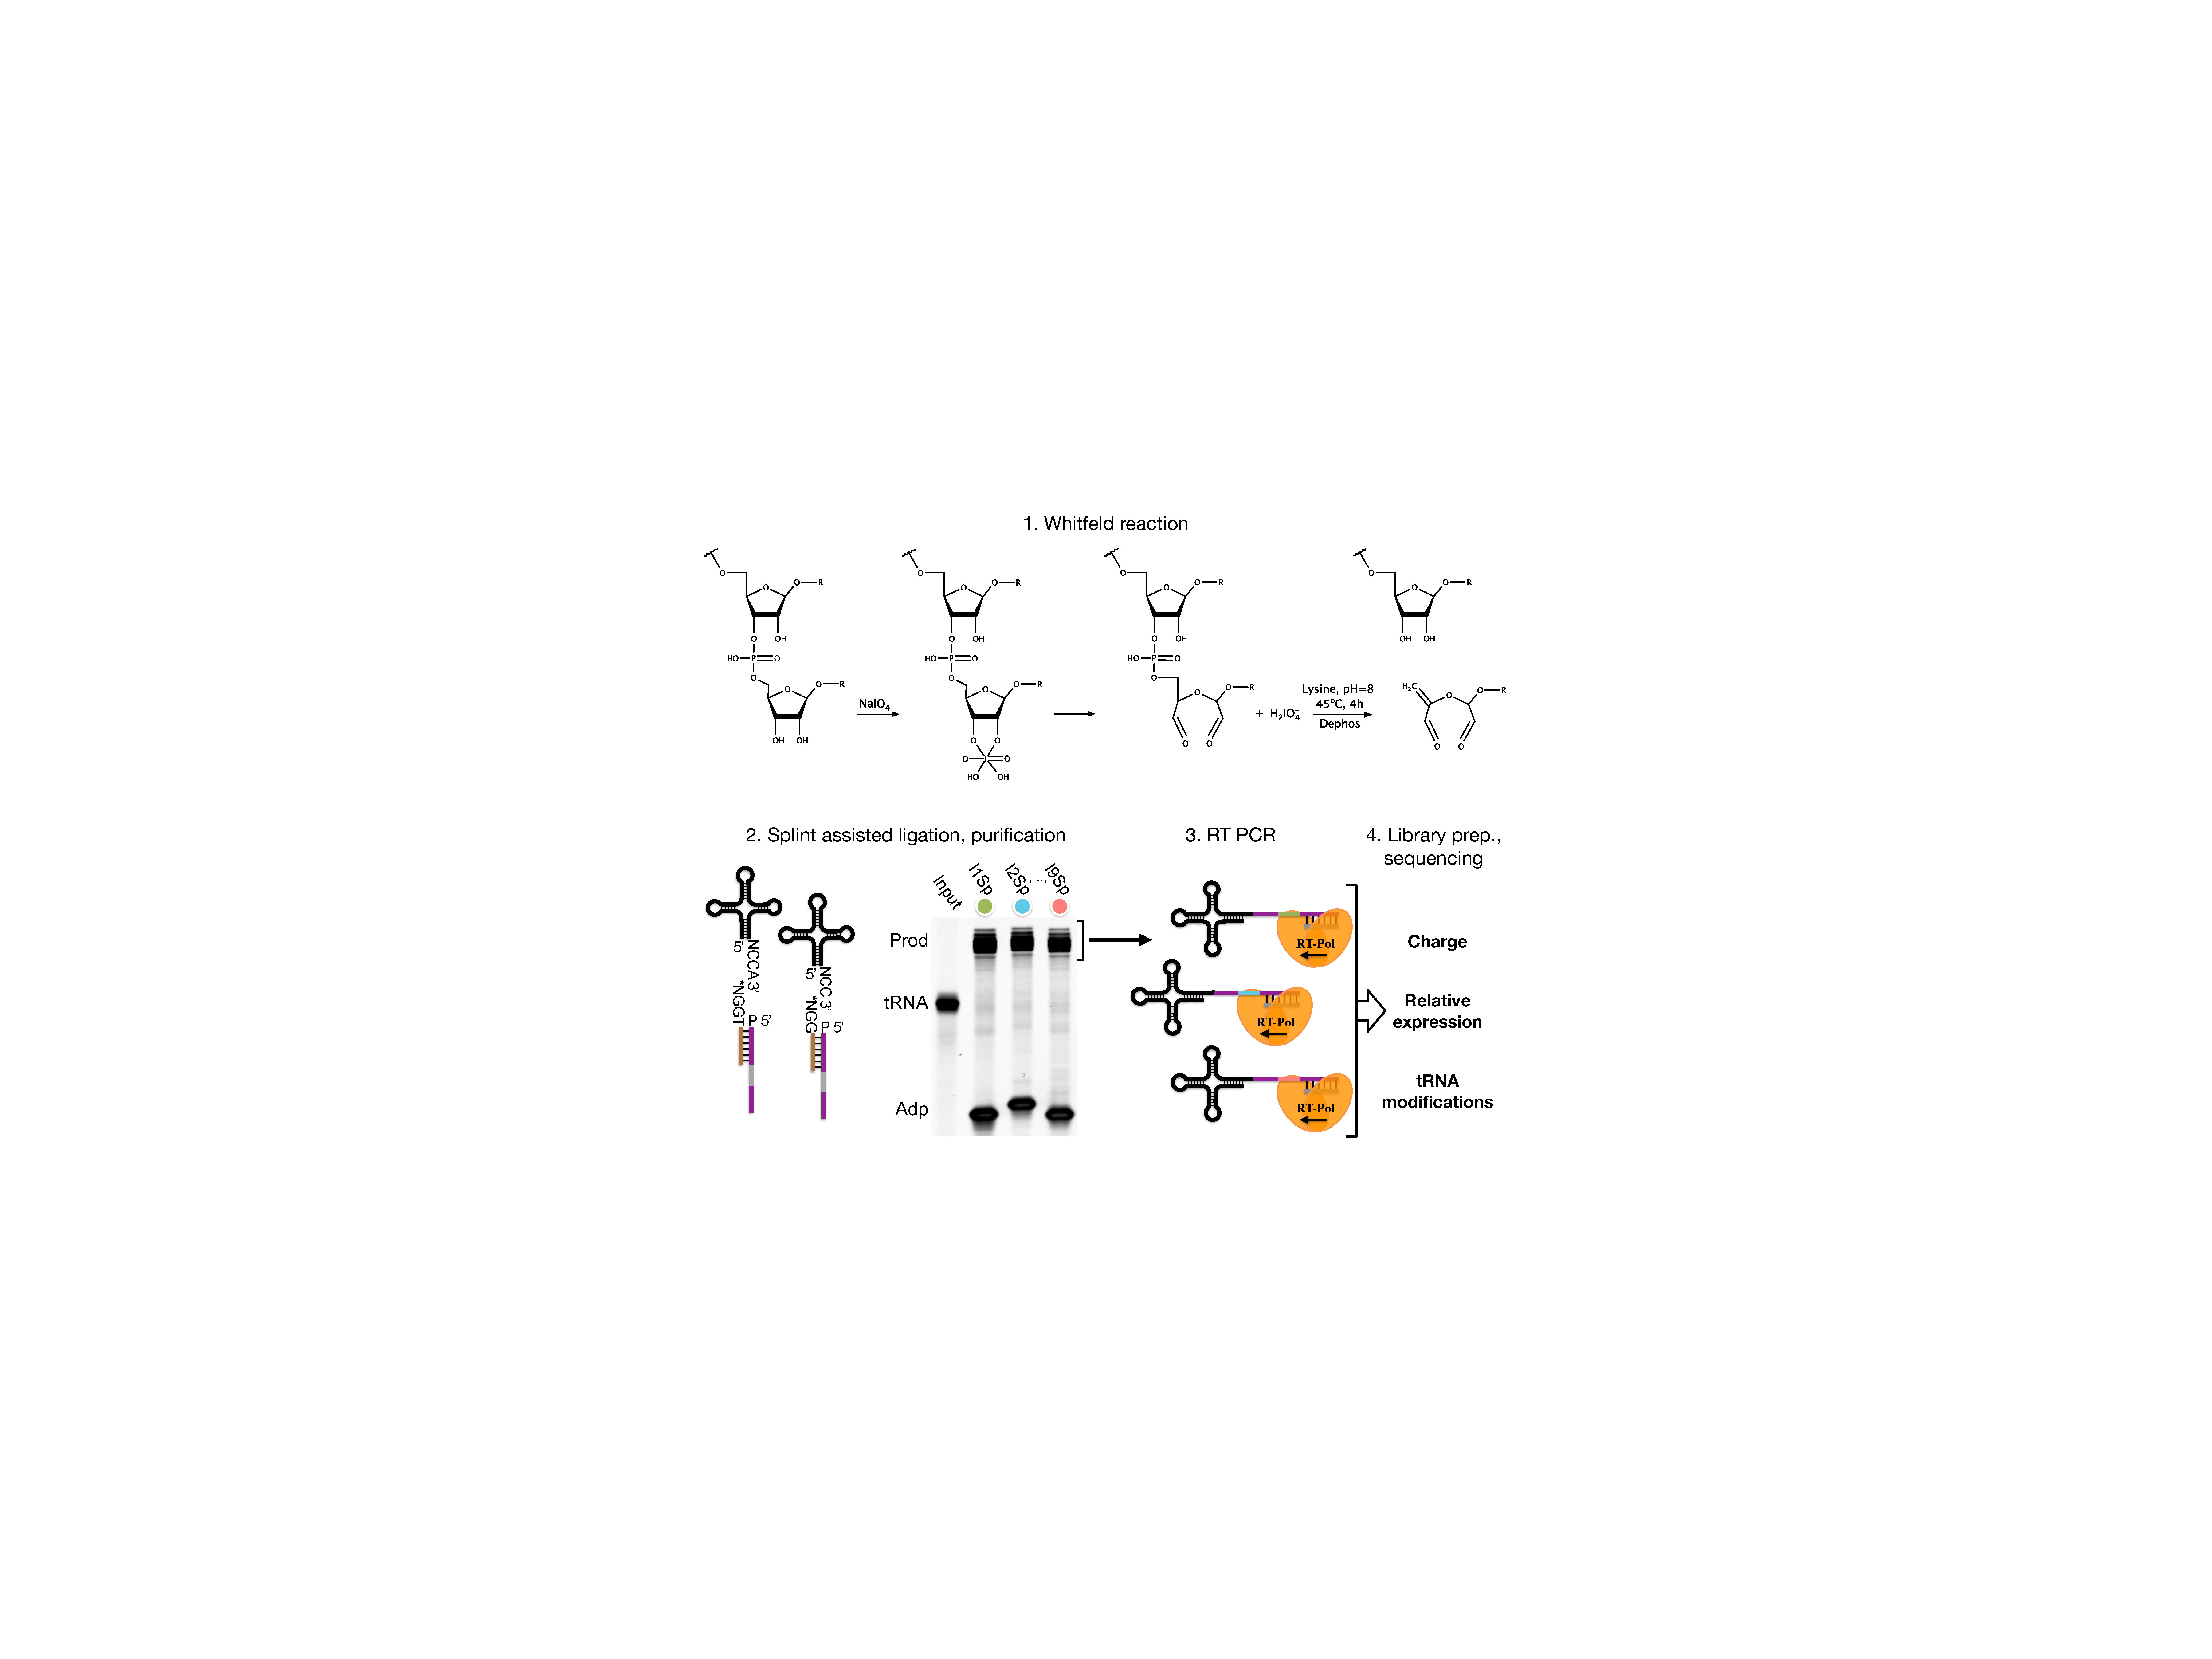
\includegraphics[width=0.7\linewidth]{figures/Fig1.pdf}}
\caption{
Summary illustrating the steps of the charge tRNA-Seq method we used to measure aminoacylation, relative expression and tRNA modification levels.
First, the Whitfeld reaction (detailed in \FIGSUPP[Fig1]{f1S1}) is used to discriminate between tRNAs with and without an aminoacylation by cleaving off the 3′ base of deacylated tRNA.
Second, the tRNA is folded to expose the discriminator base (N) followed by the CCA/CC-end, creating a sticky-end for splint assisted ligation to a barcoded adapter.
Stars (*) on the 3′ end of splint and adapter oligos indicate modifications to block self-ligation.
Third, using the purified ligation product, RT-PCR is used to generate cDNA.
Fourth, the cDNA is converted into a dsDNA library and sequenced to determine tRNA charge, expression and modifications.
}
\label{fig:Fig1}

\figsupp[Whitfeld reaction scheme.]{
Schematic of the Whitfeld reaction with acylated and deacylated tRNA leading to generation of CCA and CC-ending tRNAs.
For deacylated tRNA, 3′ adenosine is oxidized by periodate and then cleaved off by lysine induced β-elimination [references].
Acylated tRNA is protected from periodate oxidation but will be deacylated in the subsequent incubation with lysine.
}{\fbox{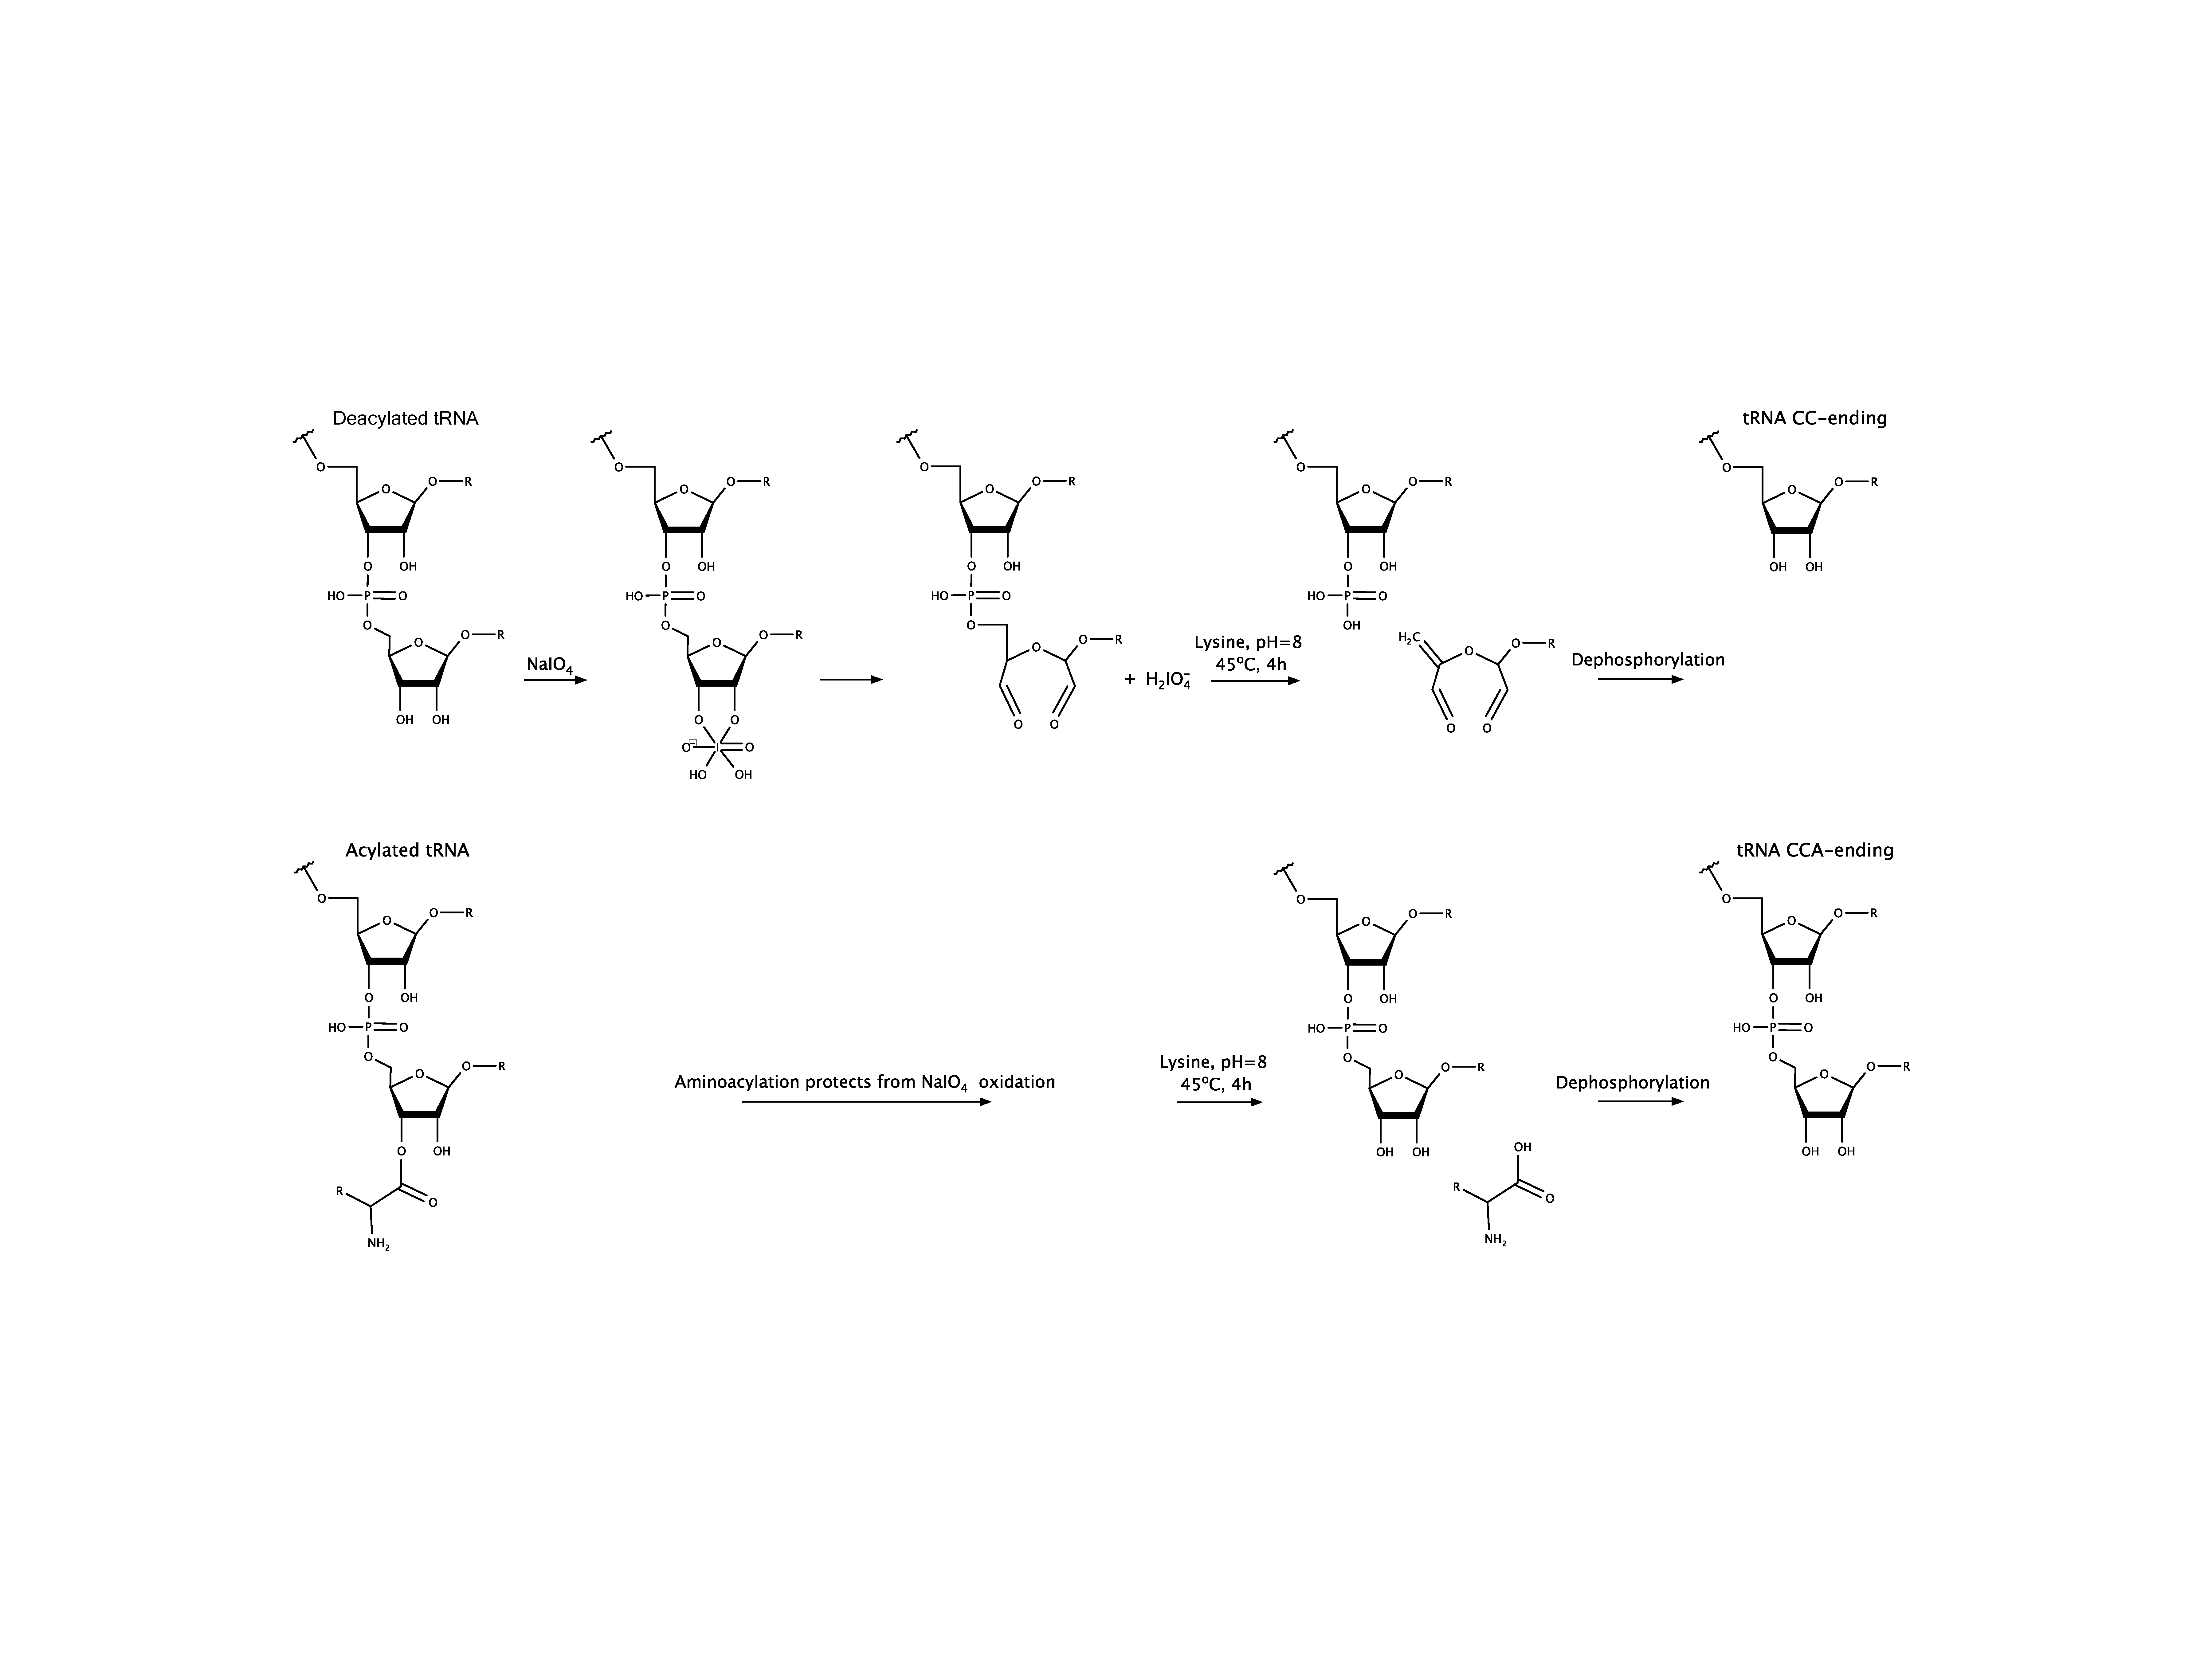
\includegraphics[width=0.9\linewidth]{figures/Fig1S1.pdf}}}\label{figsupp:f1S1}
\end{figure}




\section{Results}
\subsection{Optimizing the Whitfeld reaction for charge tRNA-Seq}
The use of periodate oxidation to discriminate aminoacylated tRNA was first used by \cite{Dittmar2005-va} for microarray measurements and then elegantly adapted to high-throughput sequencing by \cite{Evans2017-st}.
However, we found noticeable differences between the conditions reported optimal for periodate oxidation in biochemical assays in the past \citep{Khym1961-xf, Neu1964-hu, Khym1968-ac, Dyer1956-zh} and those used in charge tRNA-Seq today \citep{Evans2017-st, Behrens2021-gb, Watkins2022-er, Pavlova2020-aj, Tsukamoto2022-rc}.
We therefore reasoned that it would be valuable to find a set of optimal conditions for the Whitfeld reaction when applied to charge tRNA-Seq.
To do this, we used an E.coli tRNA-Lys-CCA oligo and measured conversion to its 1 nt. truncated product.

Periodate oxidation of cis-glycols is known to occur rapidly, even at low temperature \citep{Dyer1956-zh}; therefore, we tested if oxidation could be performed on ice to protect tRNA aminoacylations prone to hydrolysis.
We found that complete oxidation is achieve after just 5 min (\FIG{Fig2}, panel A) and therefore chose 10 min as optimal, with incubation on ice and in the dark because sunlight induces periodate oxidation side-reactions \citep{Erskine1953-cr}.

Oxidation of deacylated tRNA yields a dialdehyde on the terminal ribose which enables the phosphoric ester linkage to be broken in a $\beta$-elimination reaction \citep{Rammler1971-mt, uziel1973periodate}, yielding an unsaturated product (\FIGSUPP[Fig1]{f1S1}).
While this cleavage reaction is complex, involving several semi-stable intermediates and different pathways depending on the pH, it appears to be induced by high pH and the presence of a primary amine \citep{Uziel1975-ja}.
Lysine has been identified as a good source of primary amine and incubation at 45°C has been found optimal \citep{Khym1961-xf, Neu1964-hu}.
In previous charge tRNA-Seq methods, a borax buffered solution at pH=9.5 has been used to induce cleavage, instead we wanted to test using lysine at pH=8 to improve RNA stability.
We found complete cleavage after 90 min (\FIG{Fig2}, panel B); however, this step also serves as deacylation step and some aminoacylations were measurable after 90 min of lysine cleavage (\FIGSUPP[Fig2]{f2S1}, panel A).
Therefore, we settled on a 4 h incubation time, but even with this extended incubation, the decrease in pH made a large improvement on RNA integrity (\FIG{Fig2}, panel C).

Finally, we wanted to perform the Whitfeld reaction as a one-pot reaction as shown by \cite{Watkins2022-er}.
However, we found that the typically quenchers used to remove unreacted periodate, glucose or ribose, are not compatible with lysine induced cleavage (\FIGSUPP[Fig2]{f2S1}, panel C).
This is likely due to the generation of dialdehydes that cross-link lysines; therefore, we chose to use ethylene glycol which only forms formaldehyde upon periodate oxidation.
Additionally, ethylene glycol reacts fast and can be added in high molar excess without negatively affecting subsequent steps, thus enabling the whole Whitfeld reaction in one tube (\FIG{Fig2}, panel D).



\subsection{Adapter ligation introduce charge measurement bias}
Following the Whitfeld reaction tRNAs must be sequenced in order to measure aminoacylation levels.
To achieve this with enough throughout, we chose to ligate to barcoded adapters to enable sample pooling before the RT-PCR step \citep{McGlincy2017-ro}.
We followed the protocol of \cite{Behrens2021-gb}, with minor modifications to the oligo design, but found that the measured charge was highly variable between replicates and that the measurements were biased by the barcode identity to an unacceptable degree (\FIGSUPP[Fig2]{f2S2}).
We hypothesized that this is due to ligation bias commonly encountered in blunt-end ligation \citep{Fuchs2015-nb, Zhuang2012-nu, Jayaprakash2011-ab} and reasoned that increasing ligation efficiency could mitigate the bias.
However, our attempts to improved ligation efficiency failed as we were never able to reach more than $\sim$50\% ligation of the input tRNA (\FIGSUPP[Fig2]{f2S3}).




\subsection{Splint assisted ligation improves efficiency}
Inspired by \cite{Smith2015-ht} and \cite{Shigematsu2017-tv} we turned to splint assisted ligation.
This approach utilizes that tRNAs have four nucleotides protruding from the 3′ end and available for basepairing: the discriminator base, which can be any of the four RNA nucleotides, followed by the invariant CCA-end.
The splint oligo is designed to bind both the 3′ end of tRNAs and the 5′ end of an adapter (\FIG{Fig1}), thus bringing the two into proximity and increasing ligation efficiency.
However, whereas earlier uses of splint assisted ligation could assume that all tRNAs end on CCA, we have a mix of CCA and CC-ending tRNAs and therefore needed to use two splints.
As tRNAs compete for ligation it is imperative that CCA-ending tRNAs, with stronger interaction with the splint, is not favoured.
Fortunately, we observed a near complete ligation between all of our nine barcoded adapters and both CCA-ending human tRNA and a CC-ending tRNA-Lys oligo (\FIGSUPP[Fig2]{f2S4}, panel A and B).
The ligation was specific as it was fully dependent on complementarity between the tRNA and the splint (\FIGSUPP[Fig2]{f2S4}, panel C).
As we are only interested in ligation between tRNA and adapter, we block all other possible ligations through dephosphorylation of the tRNA and oligo modifications blocking the 3′ end of adapter and splint oligos.
This affords us the advantage of using a pure DNA splint without any RNA nucleotides as those used in previous publications \citep{Smith2015-ht, Shigematsu2017-tv, Pinkard2020-yd, Warren2021-wt, Thomas2021-fi, Lucas2023-vm}.

Importantly, we validated that tRNA processed using the one-pot Whitfeld reaction could be effectively used as substrate in the ligation reaction (\FIG{Fig2}, panel E).
We noted that a small amount of unligated tRNA appeared in reactions with tRNA oxidized with periodate.
This unligated tRNA is of unknown origin and largely refractory to further ligation (\FIGSUPP[Fig2]{f2S5}, panel B); however, as shown later using charge titration, this did not have a measurable impact on the accuracy of the aminoacylation measurement.



\subsection{Combining optimizations results in a robust method for measuring tRNA charge}
After combining the optimized Whitfeld reaction with subsequent splint assisted ligation, we used the RT-PCR method proposed by \cite{Behrens2021-gb} using the TGIRT polymerase \citep{Mohr2013-hu} to maximize the readthrough of modified nucleotides.
We later found that high readthrough also could be achieved using Maxima RT polymerase (\FIGSUPP[Fig2]{f2S7}).
The RT-PCR was primed by an oligo containing a 10 nt. unique molecular identifier (UMI) to diversify the sequence context for the subsequent circular ligation and allow collapsing of PCR replicates during data analysis.
A final PCR was performed to attach Illumina barcodes to pool samples for multiplex sequencing.

Using this as our final charge tRNA-Seq method, we use the E.coli tRNA-Lys-CCA oligo as a spike-in control before the Whitfeld reaction to validate near complete conversion to its CC-end, suggesting efficient periodate oxidation (\FIGSUPP[Fig2]{f2S6}, panel A).
Similarly, we validated the completeness of deacylation using deacylated controls and the integrity of the tRNA CCA-end using non-oxidized controls (\FIGSUPP[Fig2]{f2S6}, panel B and C).
We then measured the baseline charge of H1299 cells grown in DMEM using four replicates, observing excellent repeatability and high charge for most codons except tRNA\textsuperscript{Ser} codons and a tRNA\textsuperscript{Glu} codon, validating observation by \cite{Evans2017-st} (\FIG{Fig2}, panel F).

\begin{figure}[ht!]
\centering
\fbox{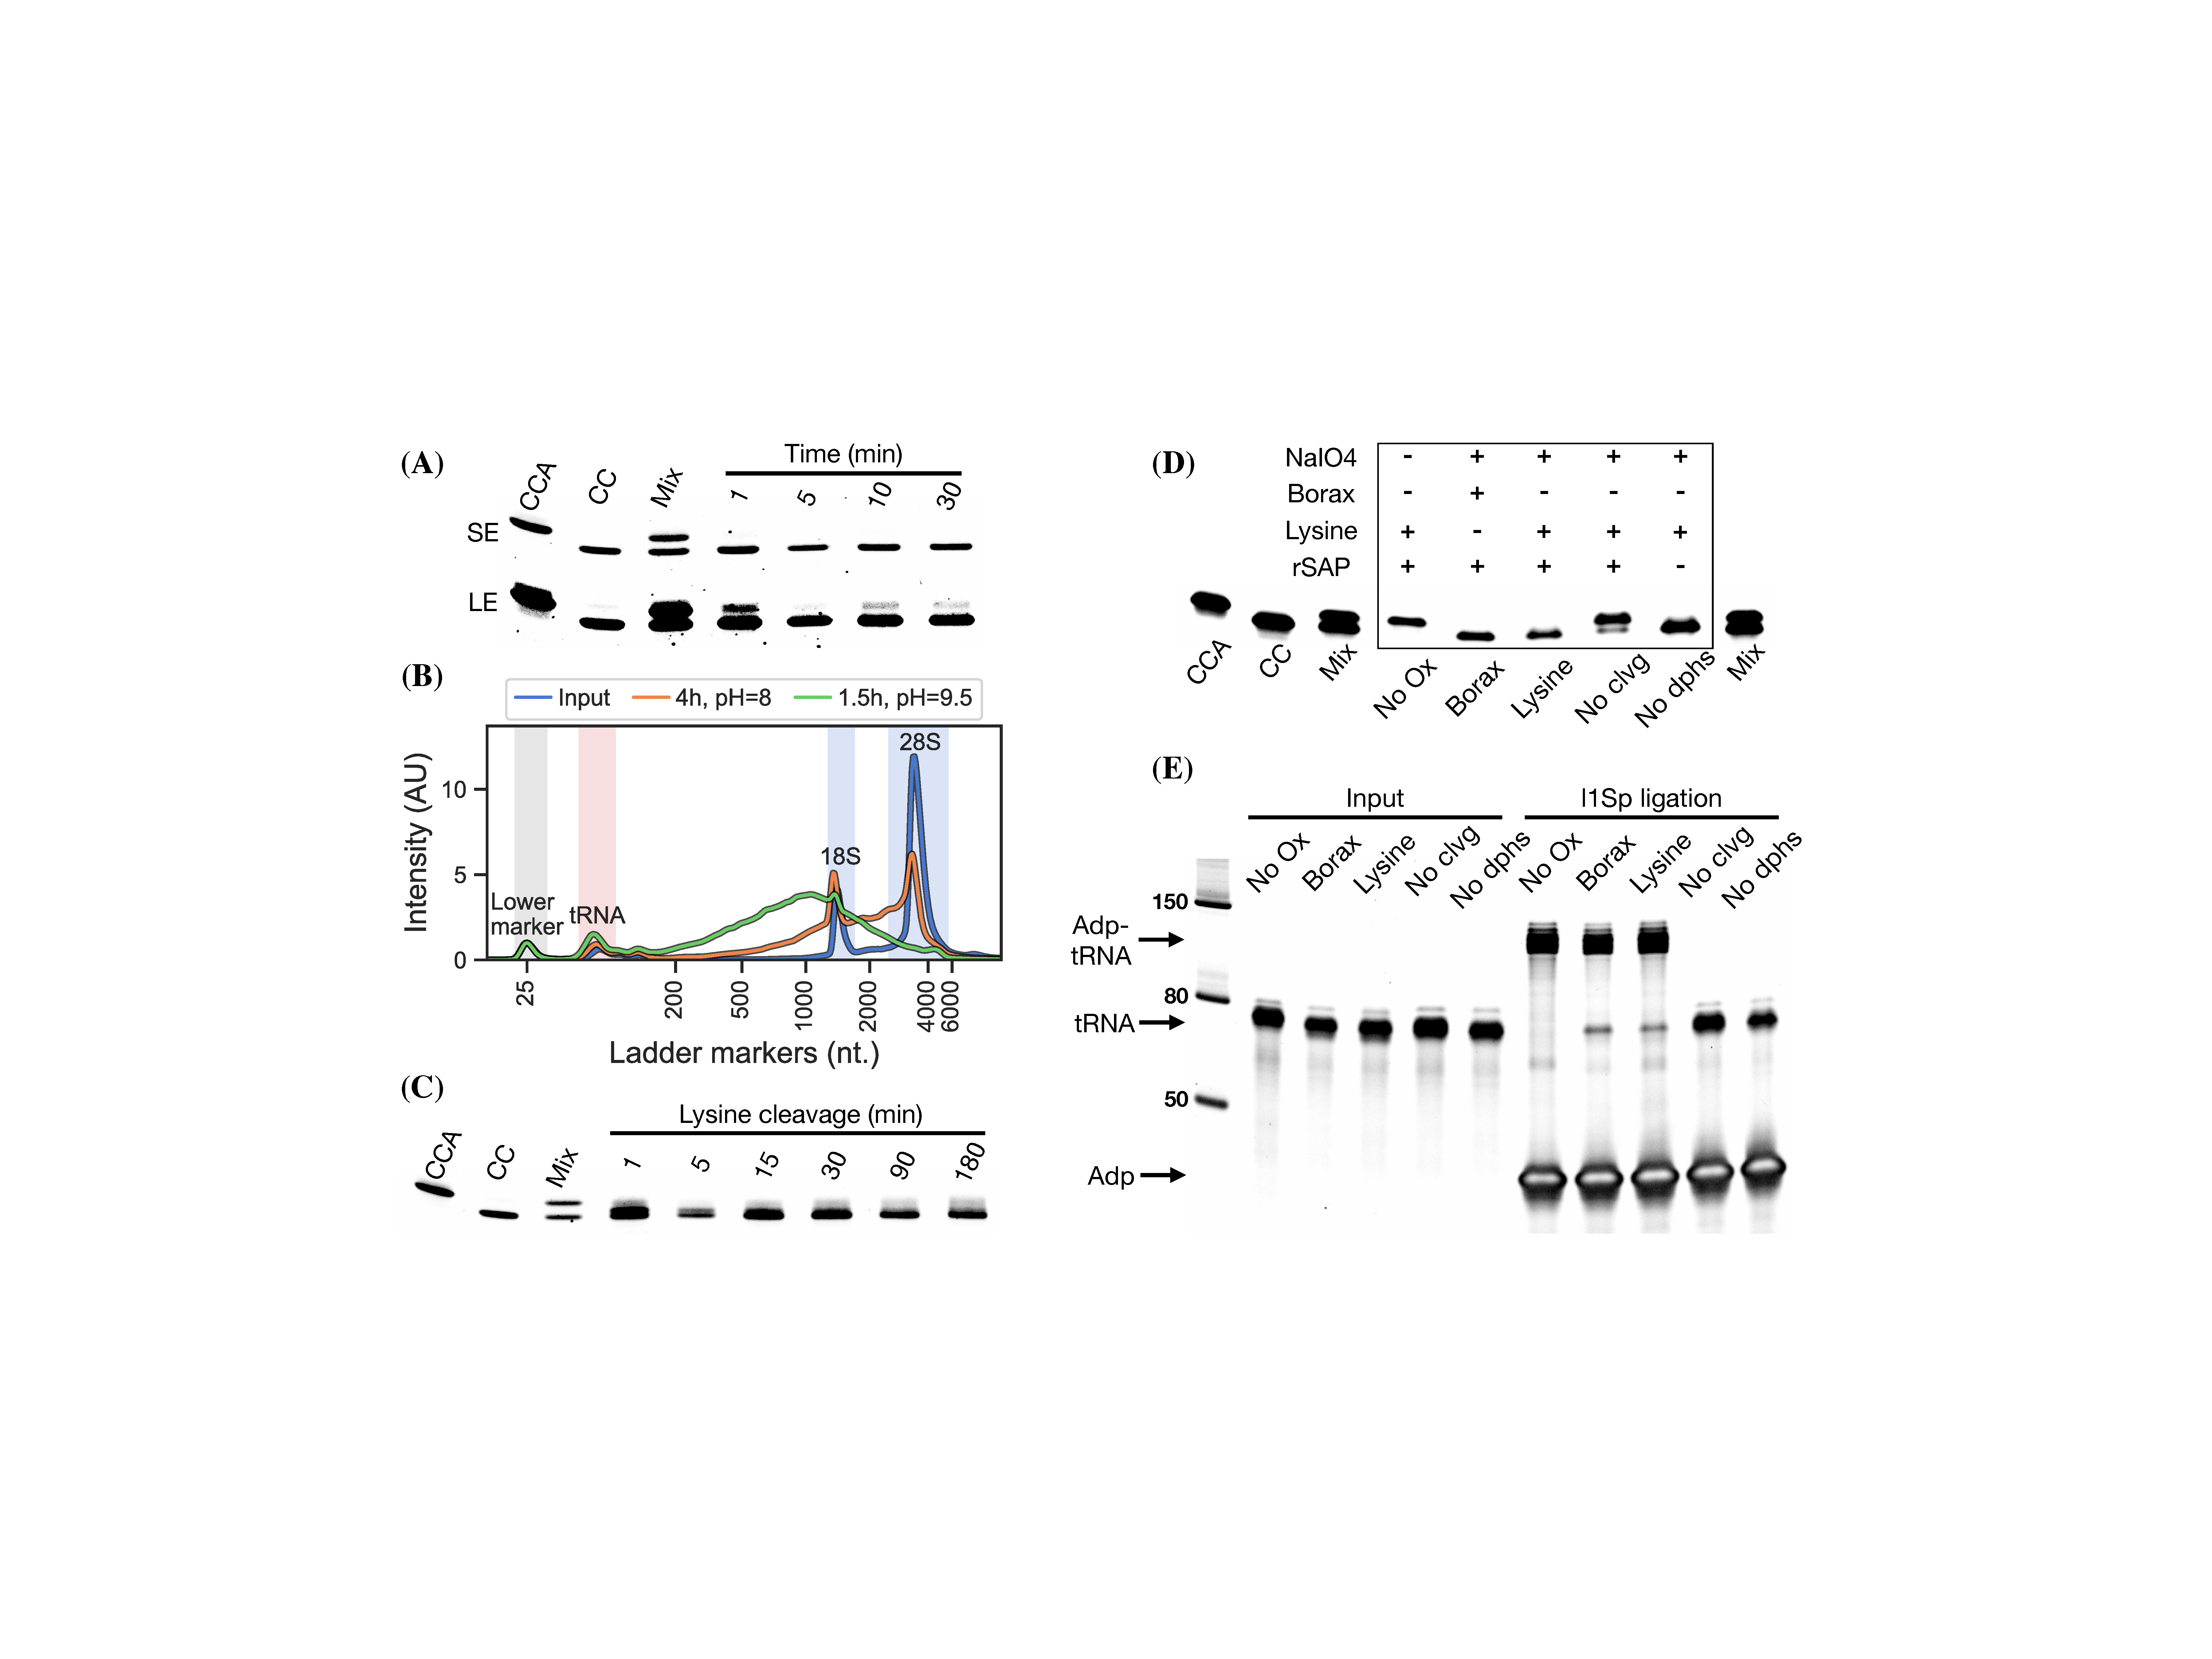
\includegraphics[width=0.8\linewidth]{figures/Fig2.pdf}}
\caption{
Optimizing the chemistry of charge tRNA-Seq.
\textbf{(A)} Time required to complete periodate oxidation of the E.coli tRNA-Lys-CCA oligo on ice.
Following oxidation, RNA was processed similar to \cite{Evans2017-st} to cleave off the 3′ adenosine.
Successful cleavage produce E.coli tRNA-Lys-CC.
CCA, input oligo.
CC, product oligo.
Mix, 50/50 mix of CCA and CC.
SE, short exposure.
LE, long exposure.
\textbf{(B)} Time required to complete lysine cleavage of the E.coli tRNA-Lys-CCA oligo (CCA) at 45°C, pH=8.
Except the cleavage step, RNA was processed similar to \cite{Evans2017-st}.
\textbf{(C)} TapeStation electropherogram comparing stability of whole cell RNA before and after 4 h lysine cleavage at pH=8 or 1.5 h borax cleavage at pH=9.5.
tRNA range marked by red background, 18/28S by blue.
See \FIGSUPP[Fig2]{f2S1}, panel B for RNA stability timecourse as it occurs on a gel.
\textbf{(D)} Effect of individual components on cleavage of the E.coli tRNA-Lys-CCA oligo (CCA).
All samples were processed as a one-pot reaction, except the borax sample which was processed similar to \cite{Evans2017-st}.
rSAP, shrimp alkaline phosphatase.
\textbf{(E)} Ligation test comparing the effect of RNA processing.
Deacylated and gel purified human tRNA was processed identically as in panel (D), then ligated to l1Sp.
Other adapters were tested with similar results (\FIGSUPP[Fig2]{f2S5}, panel A).
\textbf{(F)} Baseline tRNA aminoacylation charge in H1299 cells grown in DMEM (4 replicates, bootstrapped 95\% confidence interval of the mean).
Charge on tRNA\textsuperscript{His} is likely erroneously low because the discriminator base is shielded by base pairing \citep{Heinemann2012-hq}, creating a steric hindrance for the splint assisted ligation.
}
\label{fig:Fig2}

\figsupp[Optimizing lysine induced cleavage.]{
Optimizing lysine induced cleavage for the charge tRNA-Seq method.
\textbf{(A)} Measured aminoacylation level after 5, 30, 90 and 270 min of deacylation in 1 M lysine pH=8 at 45°C.
After deacylation, RNA was purified and submitted to the Whitfeld reaction using lysine cleavage at pH=9.5 for 90 min at 45°C to ensure complete deacylation.
The RNA was then processed using the described charge tRNA-Seq method.
\textbf{(B)} RNA stability over time for lysine cleavage at pH=8 and borax cleavage at pH=9.5.
\textbf{(C)} Lysine reacts with dialdehydes forming from quencher oxidation.
One-pot Whitfeld reactions were performed at pH=8 and pH=9.5 and quenched with either glycerol (Gly), glucose (Glc), ribose (Rib) or uridine (Urd) at concentrations indicated.
Pictures taken after the lysine cleavage step indicate side product formation consistent with lysine reacting with dialdehydes formed during the periodate quenching \citep{Saraiva2006-gw}.
This side product causes problems in the later purification step.
}{\fbox{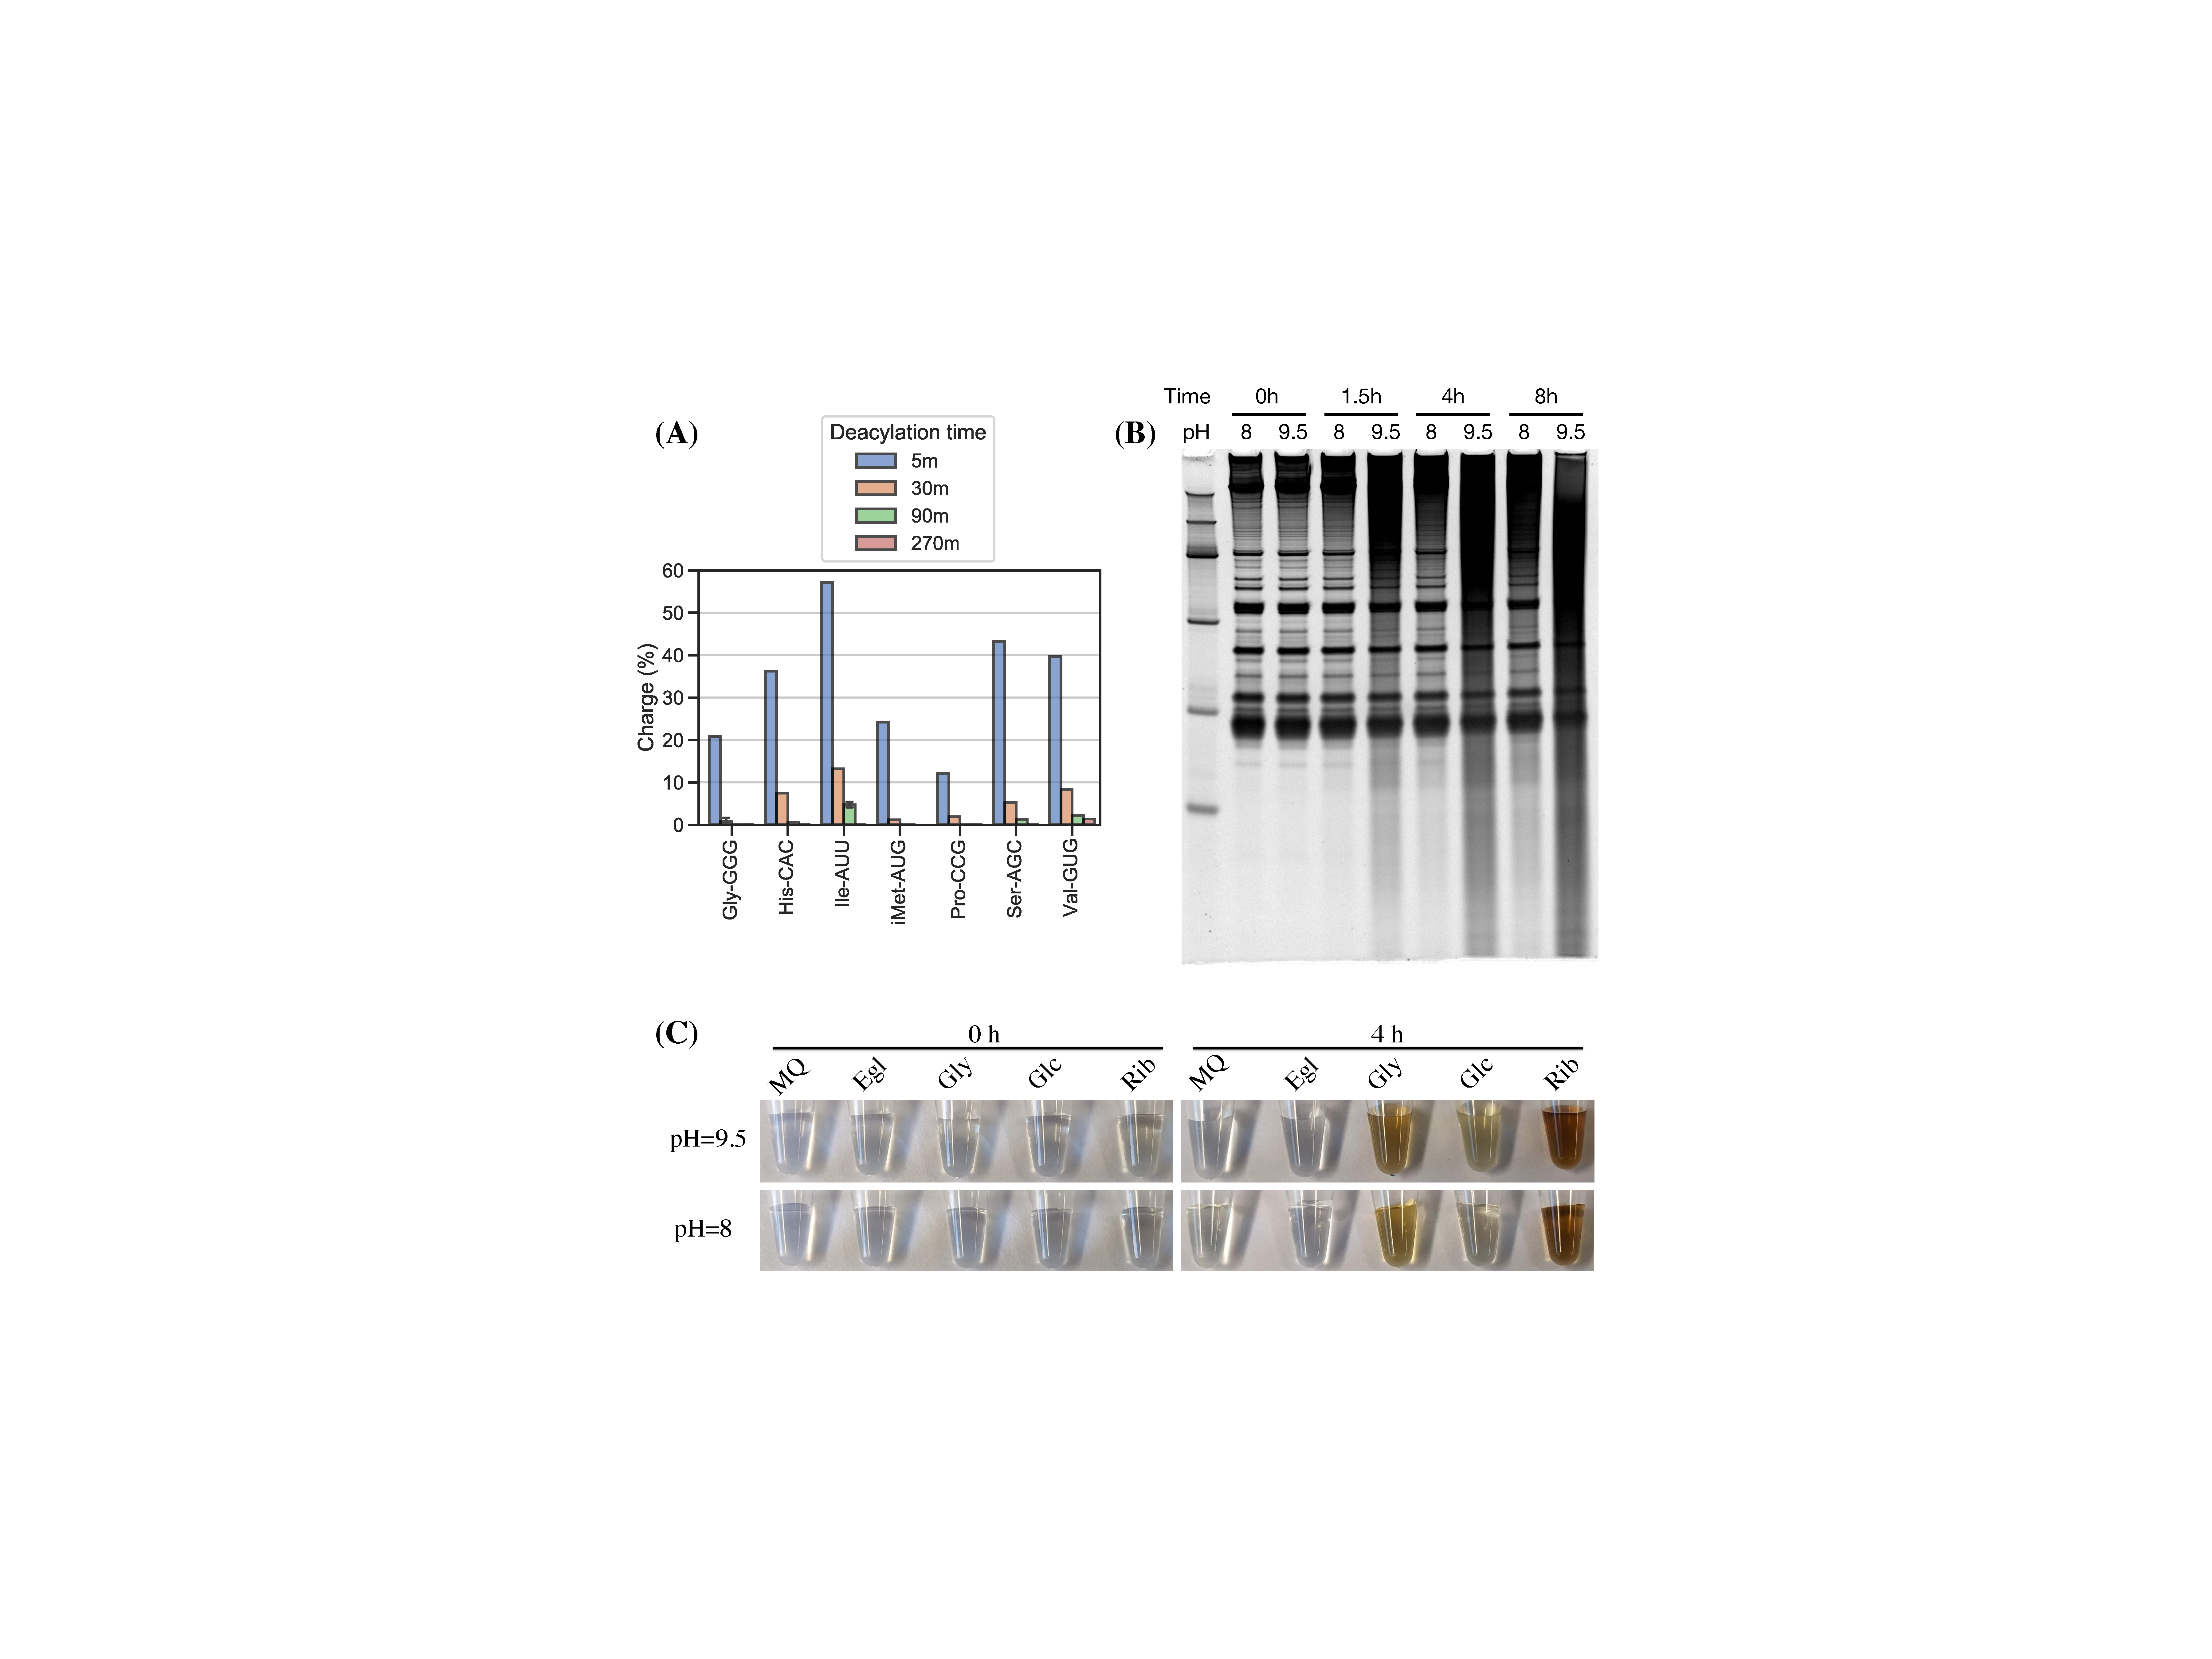
\includegraphics[width=0.6\linewidth]{figures/Fig2S1.pdf}}}\label{figsupp:f2S1}

\figsupp[Measurement bias in charge tRNA-Seq using blunt-end ligation.]{
Measurement bias in charge tRNA-Seq using blunt-end ligation.
\textbf{(A)} Measured charge of a E.coli tRNA-Lys oligo control spiked into samples processed with four different pre-adenylated adapters using the method described by \cite{Behrens2021-gb}.
The control was made using a mix of 50\% E.coli tRNA-Lys-CCA and 50\% E.coli tRNA-Lys-CC and thus its charge does not refer to aminoacylation but the CCA/CC ratio.
\textbf{(B)} Distribution of charge differences at the transcript level among samples with two barcode replicates, comparing adapters l1 vs. l2, l2 vs. l3 and l3 vs. l4.
Deviation is reported as percentage points and the kernel density estimate (KDE) is overlaid.
}{\fbox{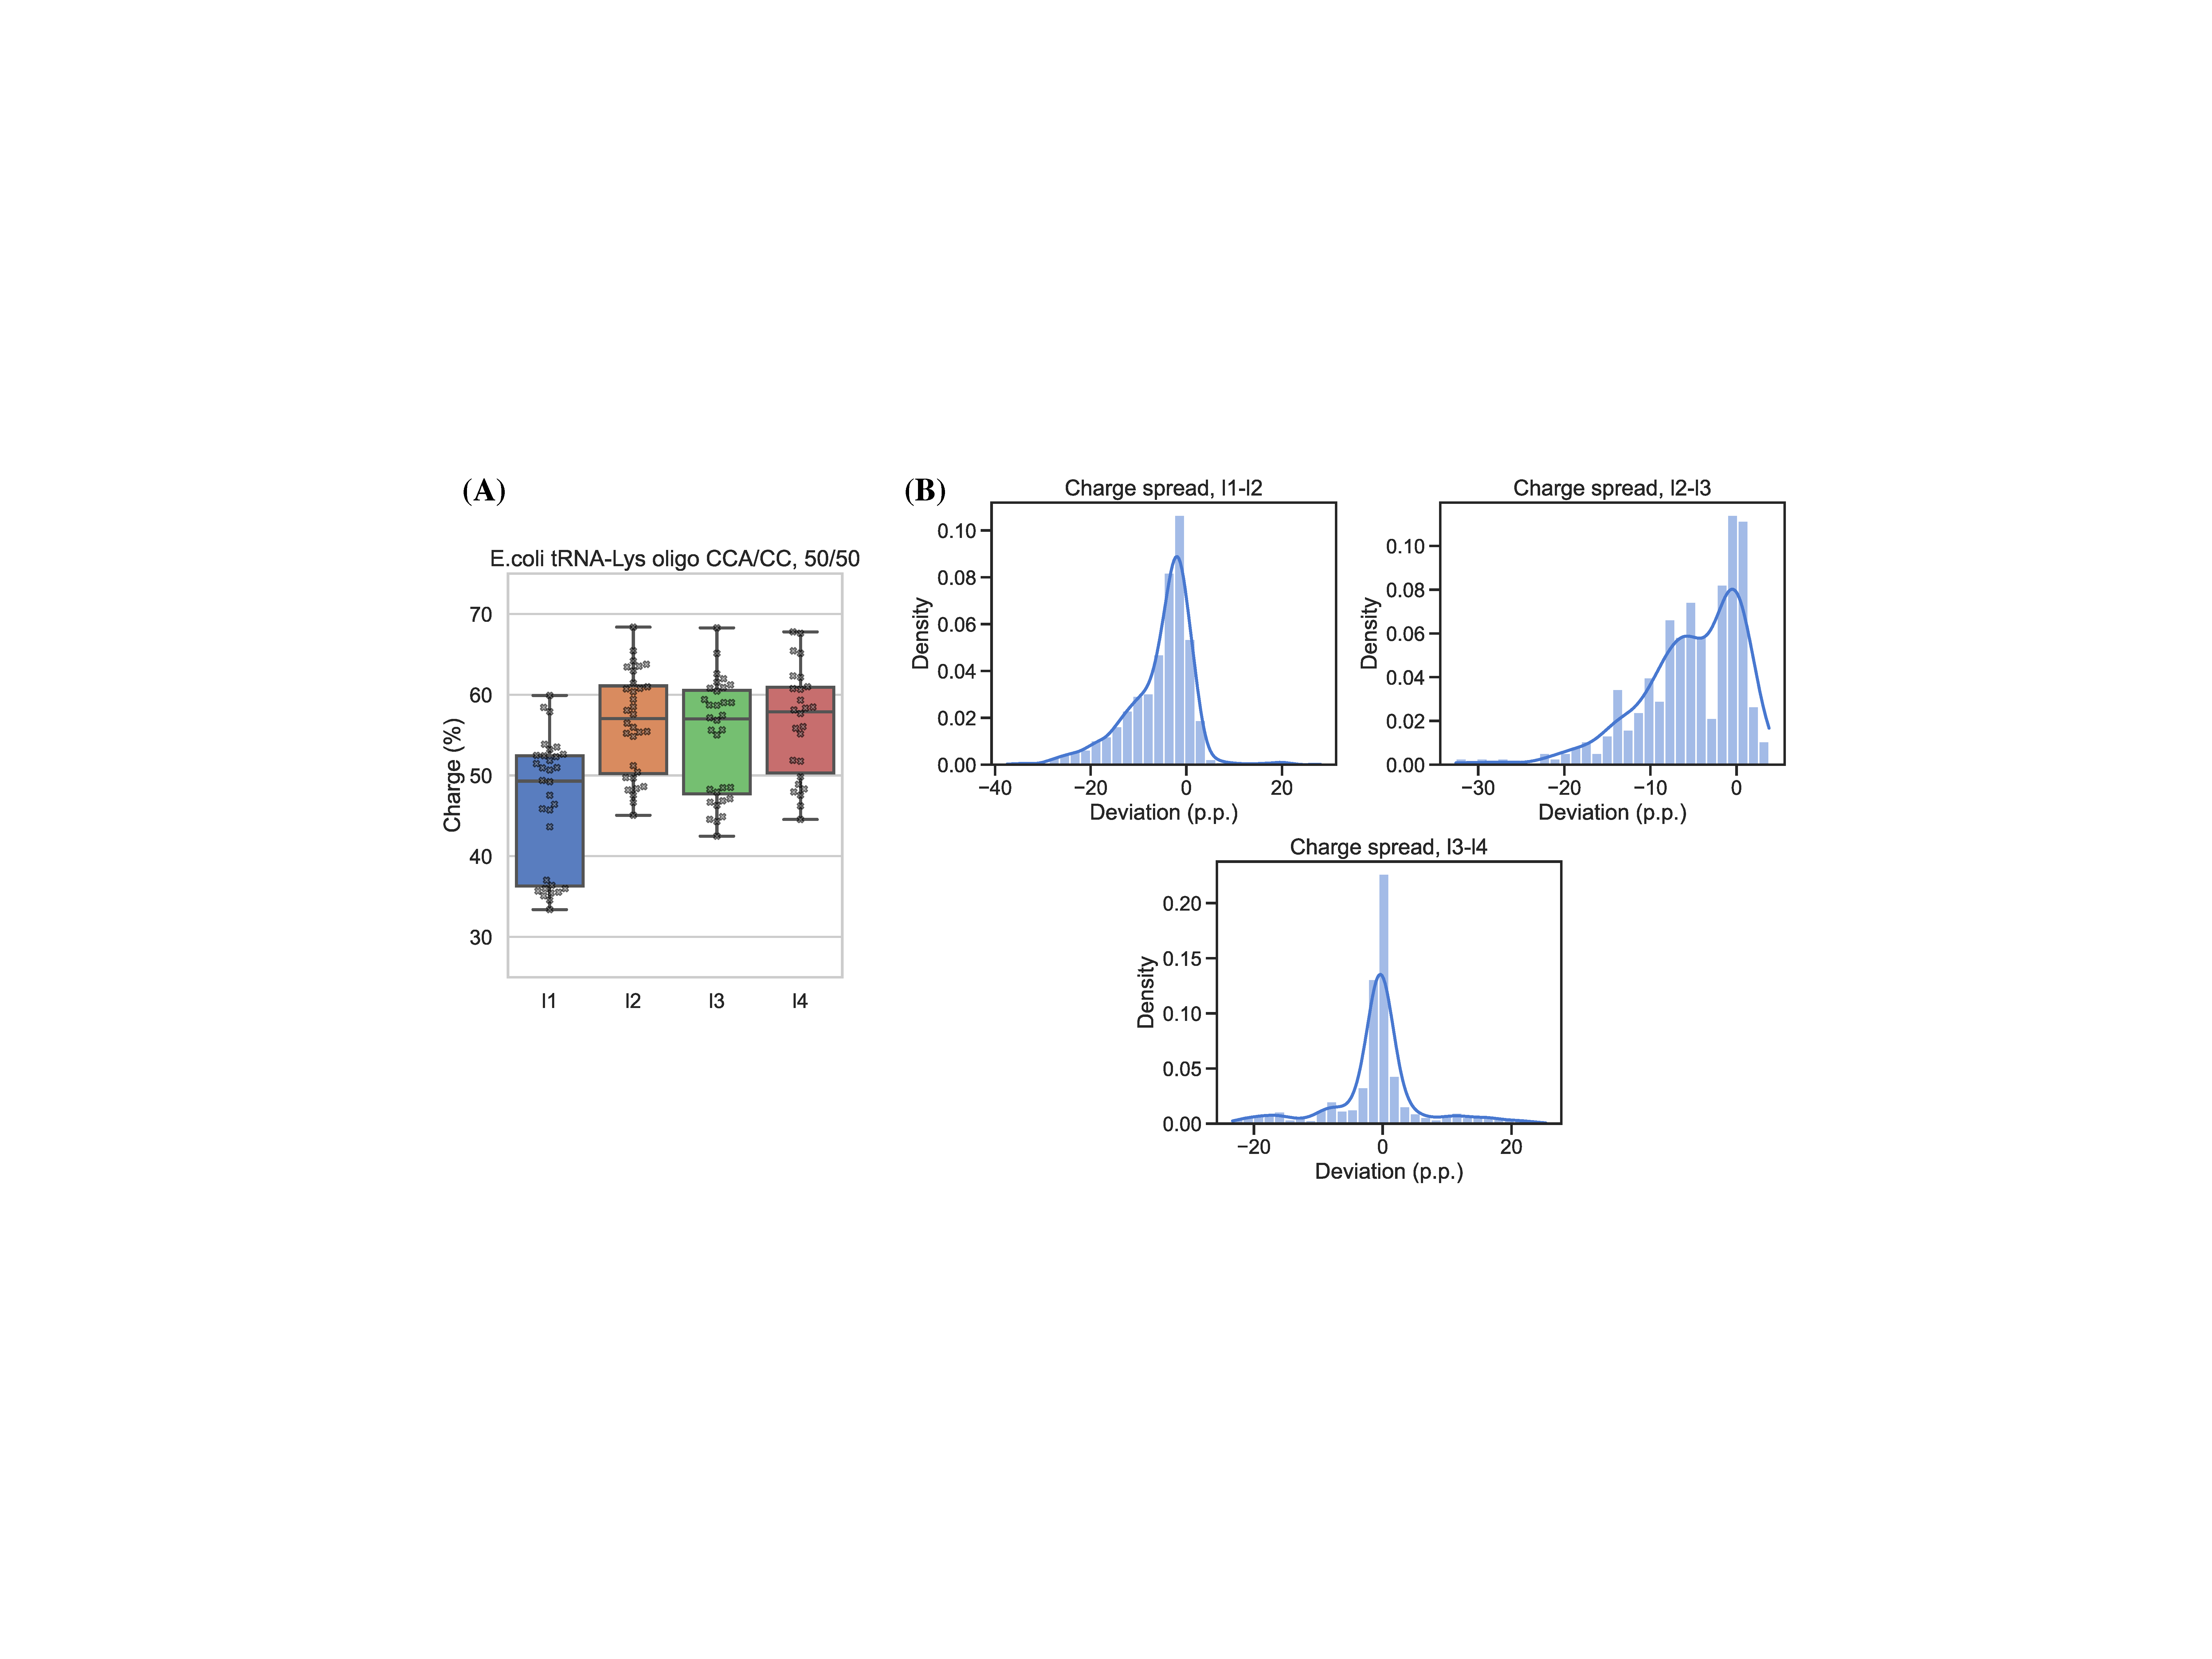
\includegraphics[width=0.8\linewidth]{figures/Fig2S2.pdf}}}\label{figsupp:f2S2}

\figsupp[tRNA-adapter blunt-end ligation attempted optimization.]{
Despite optimization attempts, high ligation efficiency could not be achieved for blunt-end ligation. 
\textbf{(A)} Effect of incubation temperature, time and addition of a phosphatase (rSAP).
Using deacylated and gel purified human tRNA as substrate and pre-adenylated l3N as adapter, otherwise following the method in \cite{Behrens2021-gb}.
\textbf{(B)} Effect of additives and higher adapter concentration.
Using deacylated and gel purified human tRNA as substrate, pre-adenylated l2N as adapter and 4°C, 24 h incubation.
An irrelevant well has been crossed out to avoid image splicing.
\textbf{(C)} Effect of ligase type.
Using the E.coli tRNA-Lys-CCA oligo as substrate, pre-adenylated l1N as adapter and 4°C, 24 h incubation with 20\% DMSO.
}{\fbox{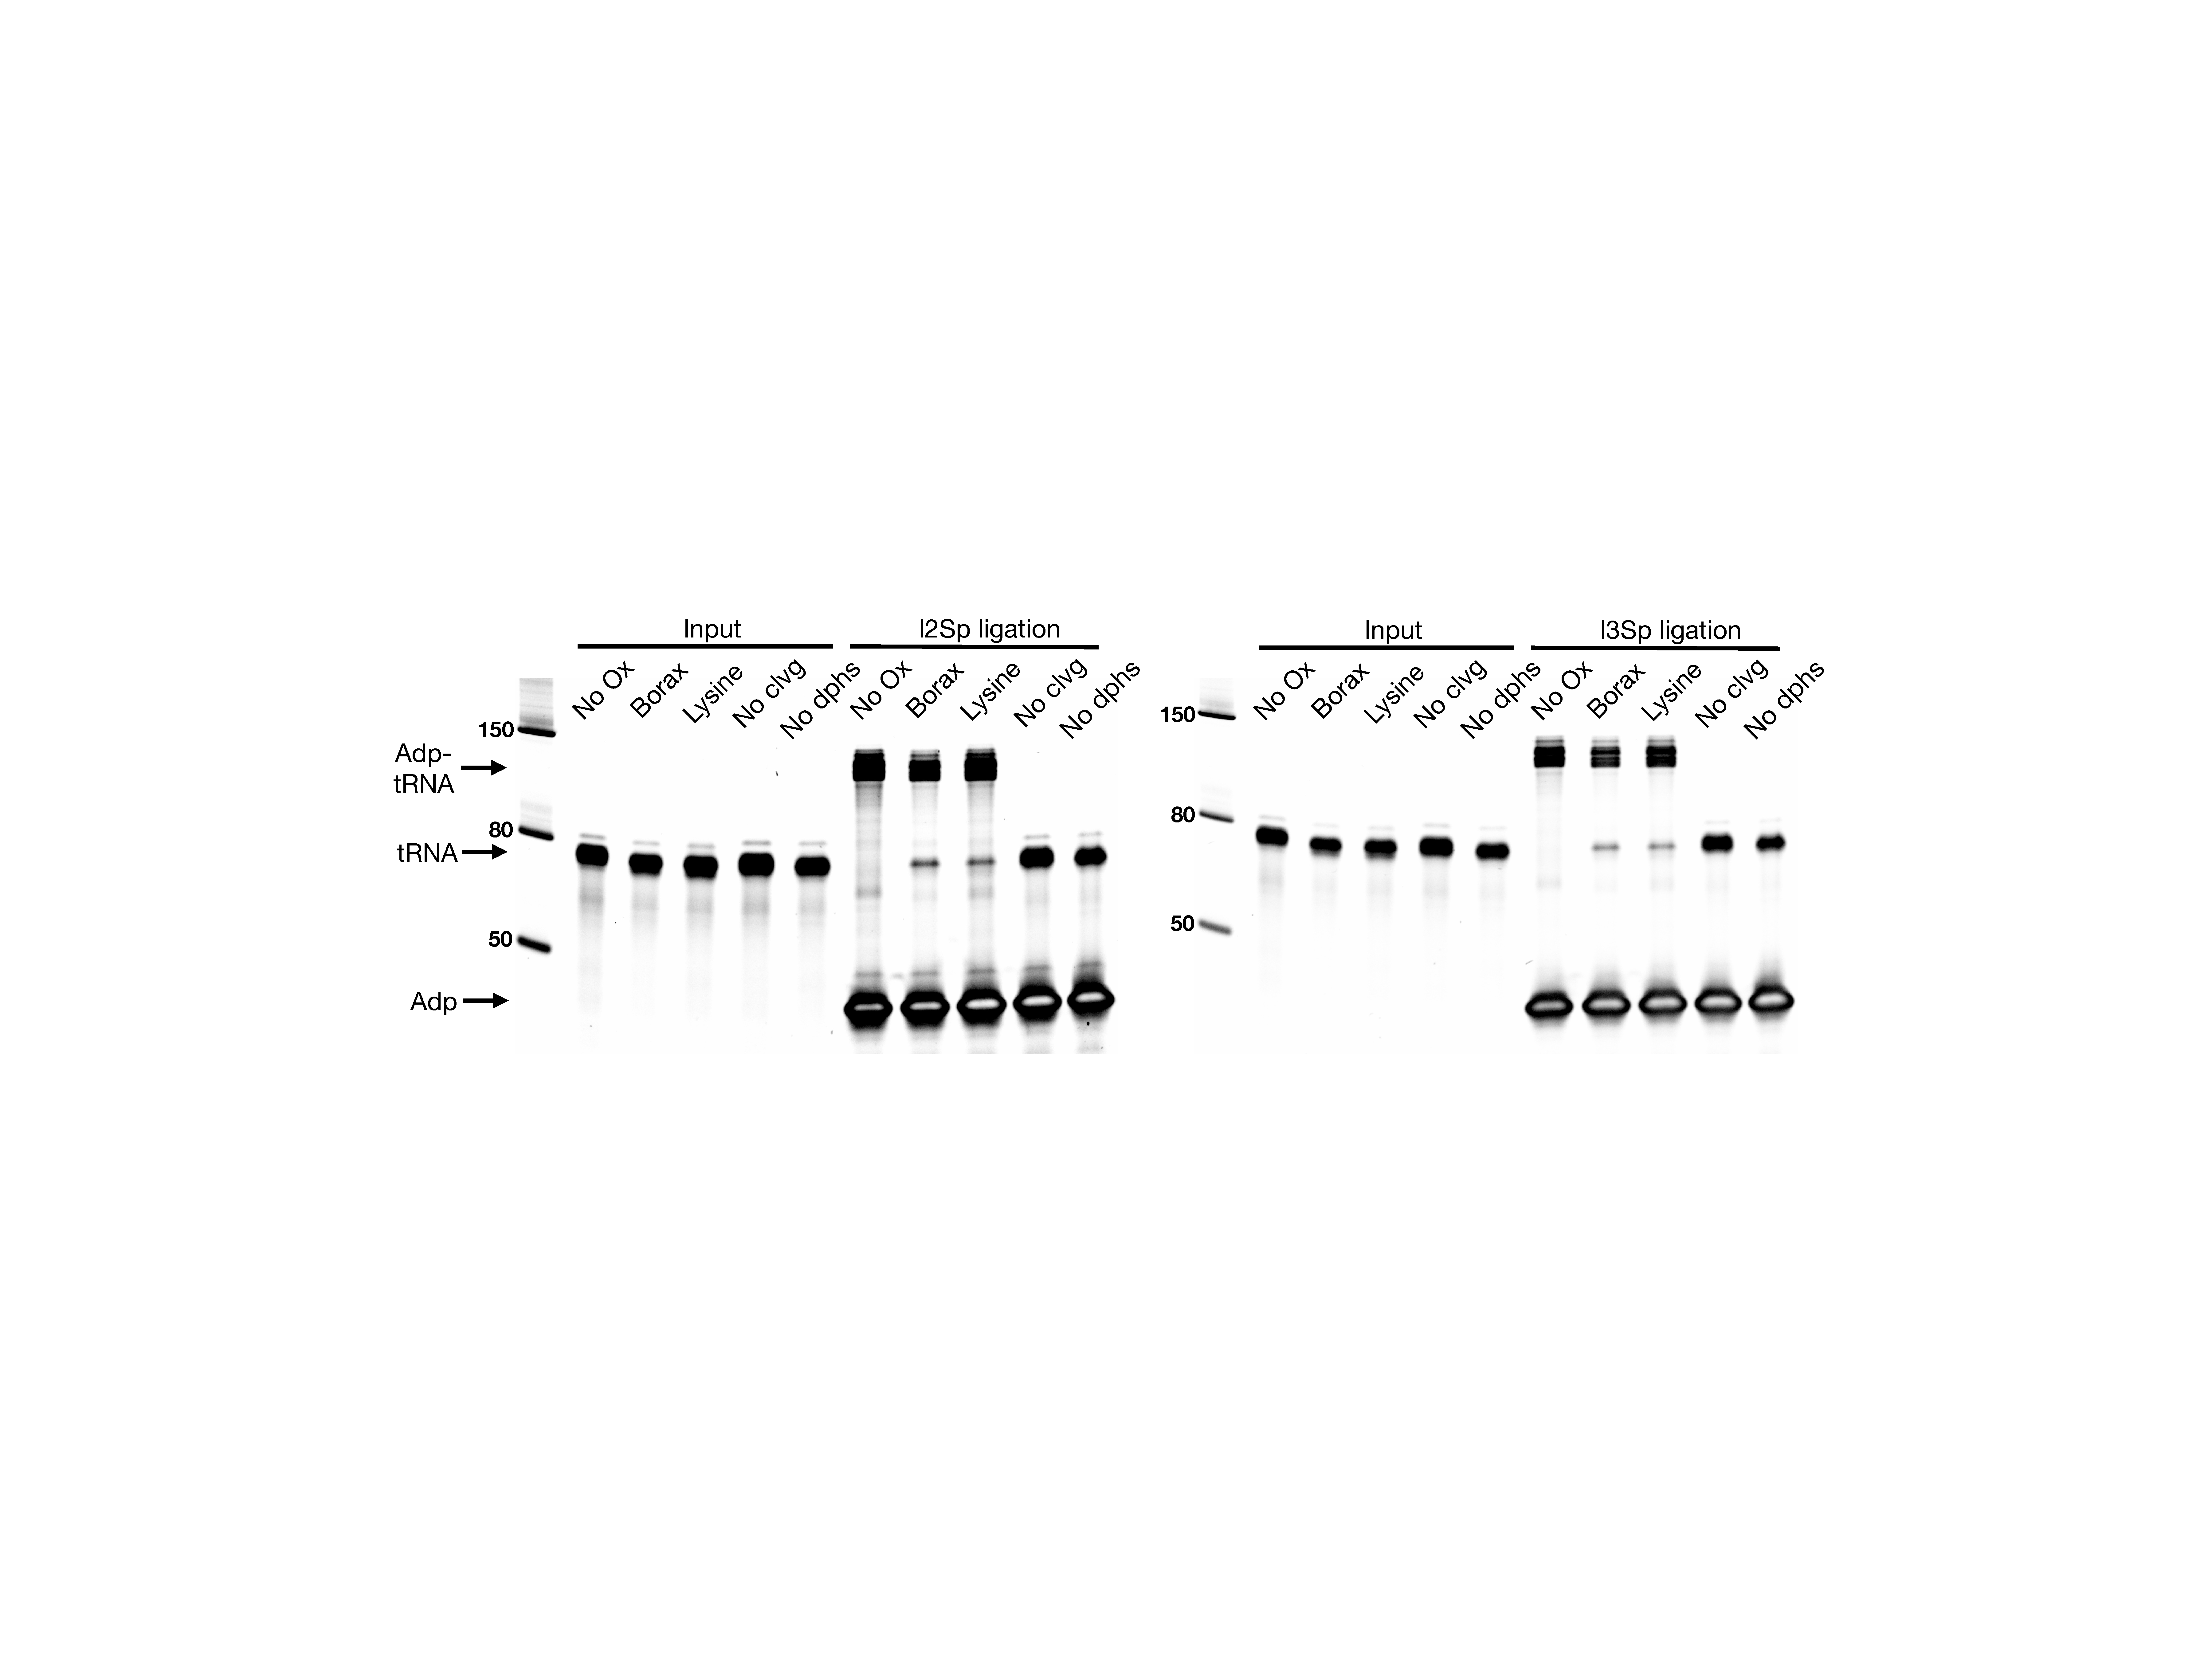
\includegraphics[width=0.85\linewidth]{figures/Fig2S3.pdf}}}\label{figsupp:f2S3}

\figsupp[Splint assisted ligation is highly efficient.]{
Ligation efficiency of all the barcoded adapters is high but depends on splint complementarity.
\textbf{(A)} Ligation reactions using deacylated purified human tRNA as substrate.
\textbf{(B)} Ligation reactions using E.coli tRNA-Lys-CC oligo as substrate.
\textbf{(C)} Comparing ligation using a tRNA-end complementary splint (l1Sp lane) vs. a non-complementary splint (NCMPL lane).
For both ligations the l1Sp adapter was used.
For the non-complementary splint ligation the two standard TGGN and GGN overhang generating splints were swapped by two splints generating CAAC and AAC overhangs.
}{\fbox{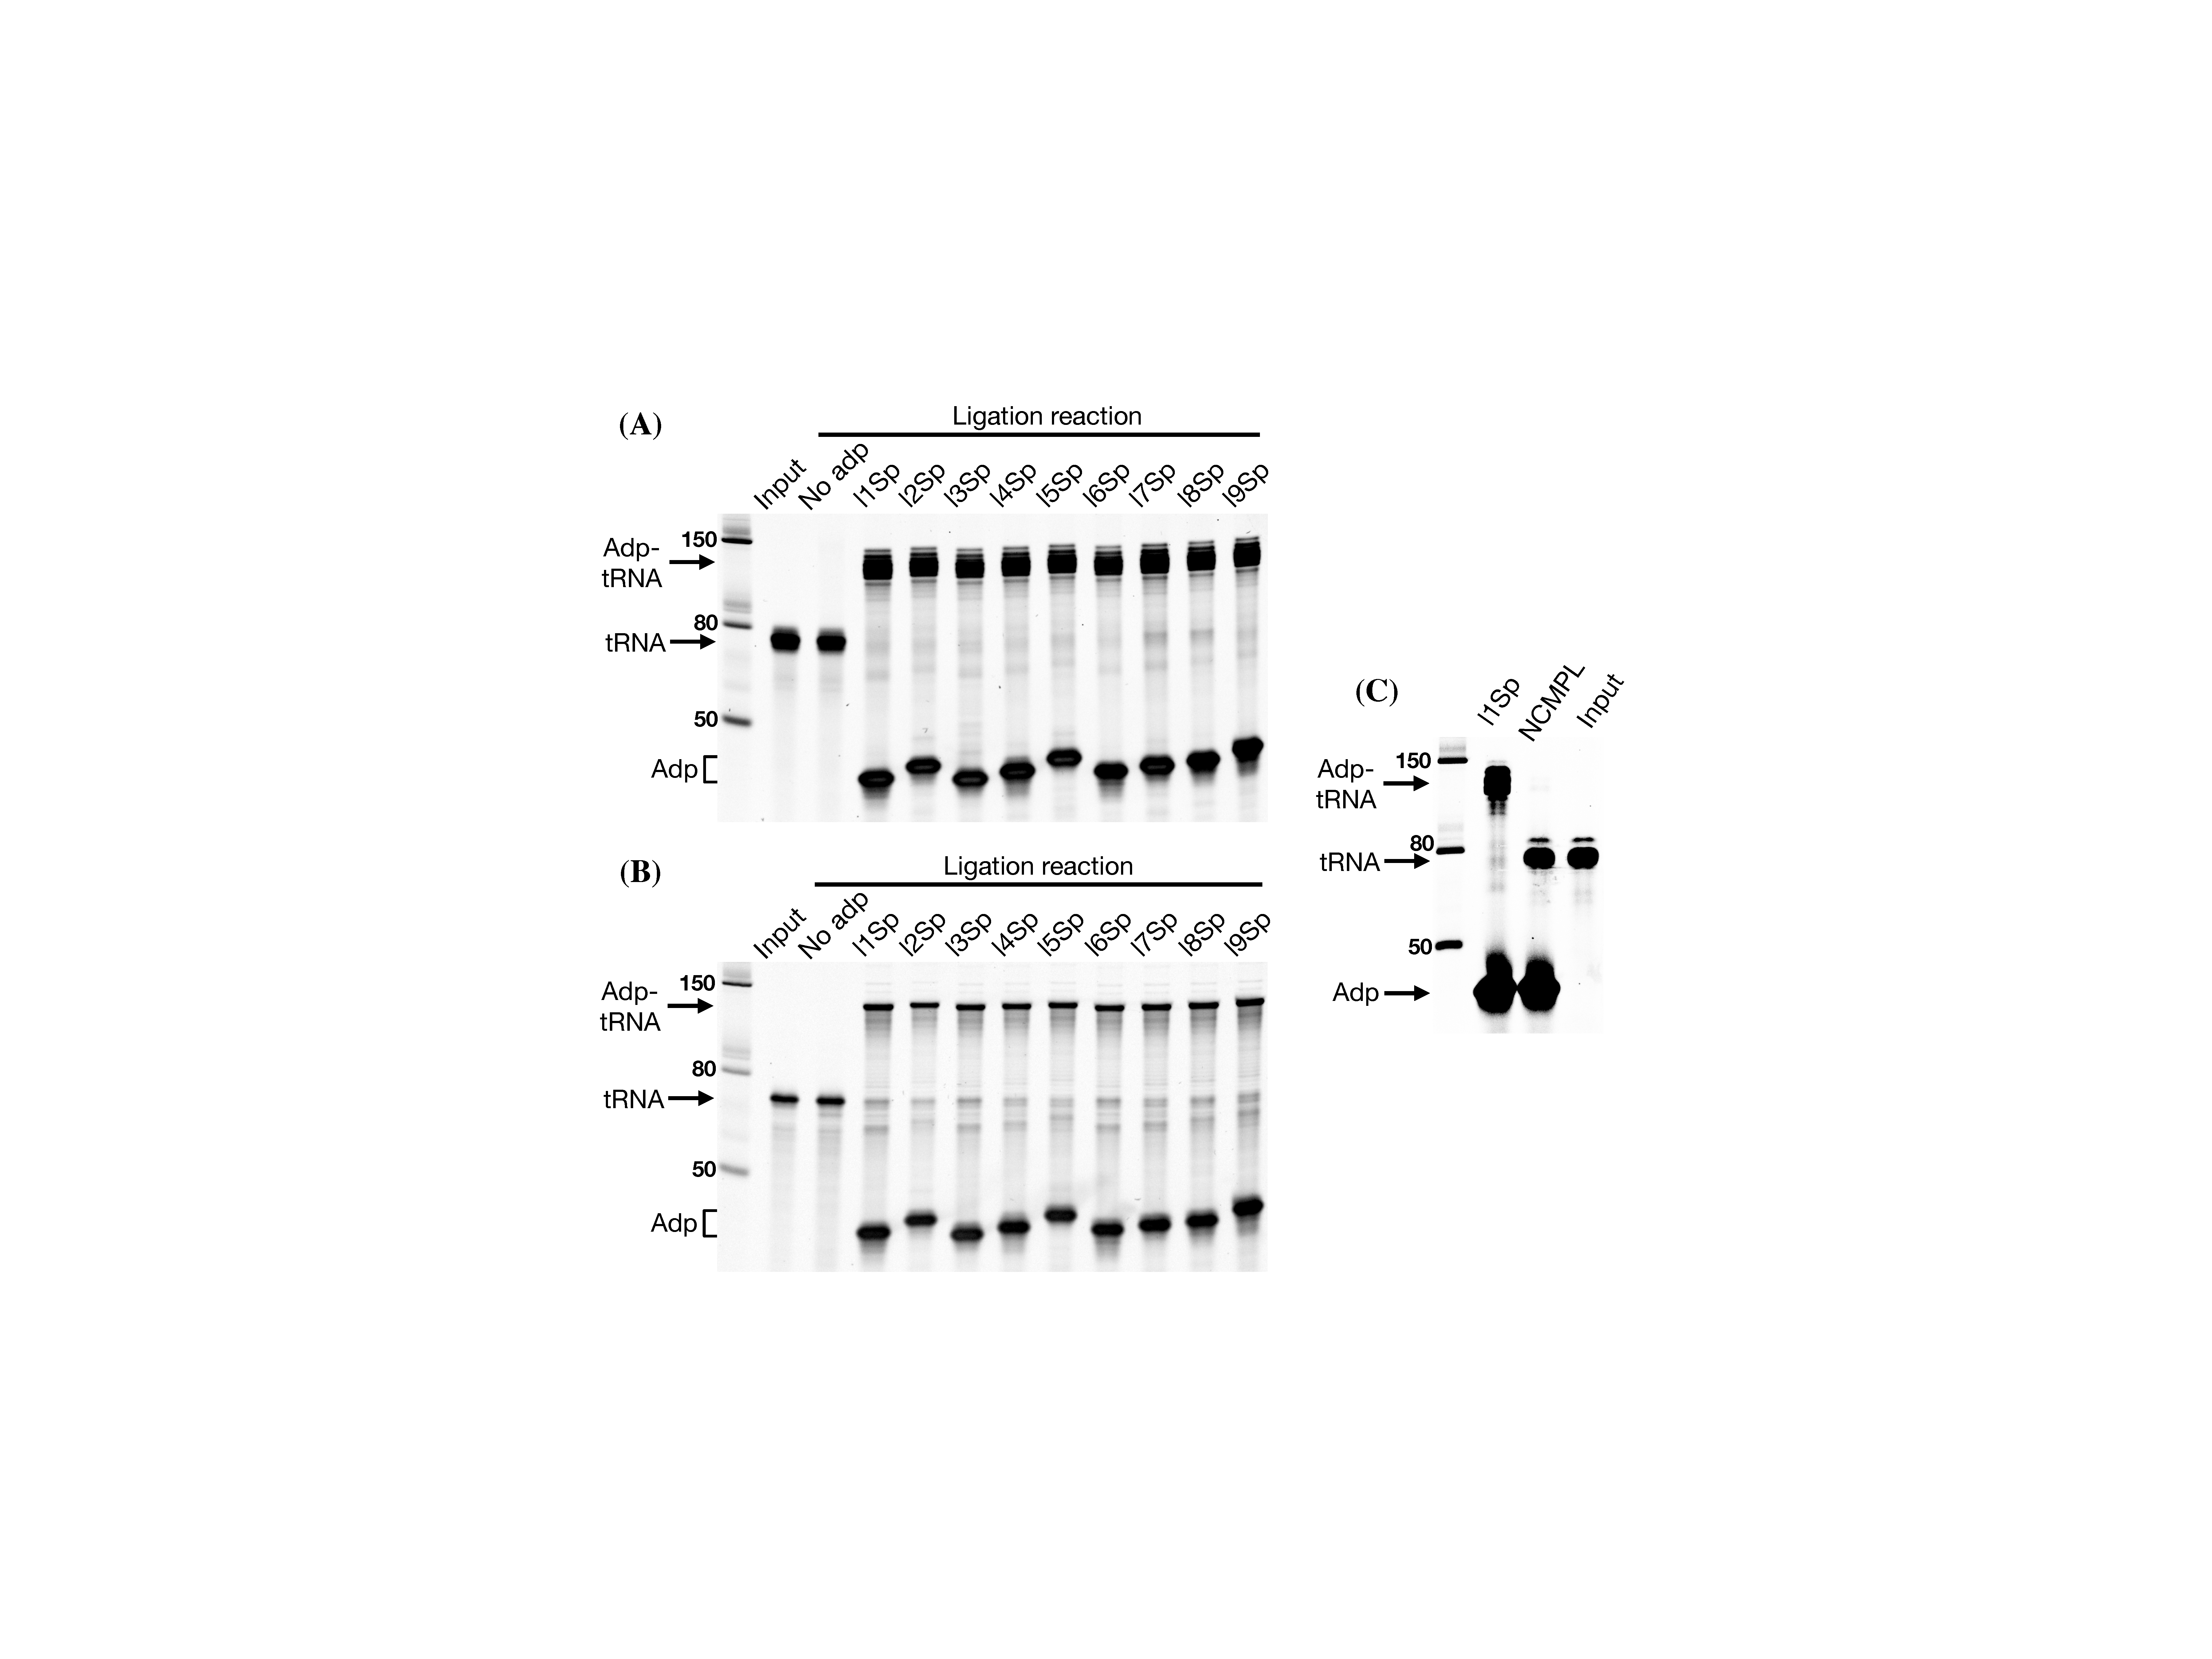
\includegraphics[width=0.7\linewidth]{figures/Fig2S4.pdf}}}\label{figsupp:f2S4}

\figsupp[Ligation tests, related to panel E.]{
\textbf{(A)} Ligation test comparing the effect of RNA processing.
Similar to \FIG{Fig2}, panel E but with two different adapters.
\textbf{(B)} The unligated tRNA that arises after tRNA is oxidized with periodate in panel A is refractory to further ligation.
The unligated tRNA was gel purified from enough ligation reactions as shown in panel A to setup two new ligation reactions using either l1N pre-adenylated adapter for blunt end ligation or l6Sp for splint assisted ligation.
For l1N, ligation was setup with 35 ng tRNA, 20 pmol adapter, 17.5\% PEG-8000, 20\% DMSO, 1xT4 RNA ligase buffer, 1 μL T4 RNA ligase 2 (truncated KQ) and 1 μL SuperaseIn.
For l6Sp, the ligation was setup as described in the charge tRNA-Seq protocol.
}{\fbox{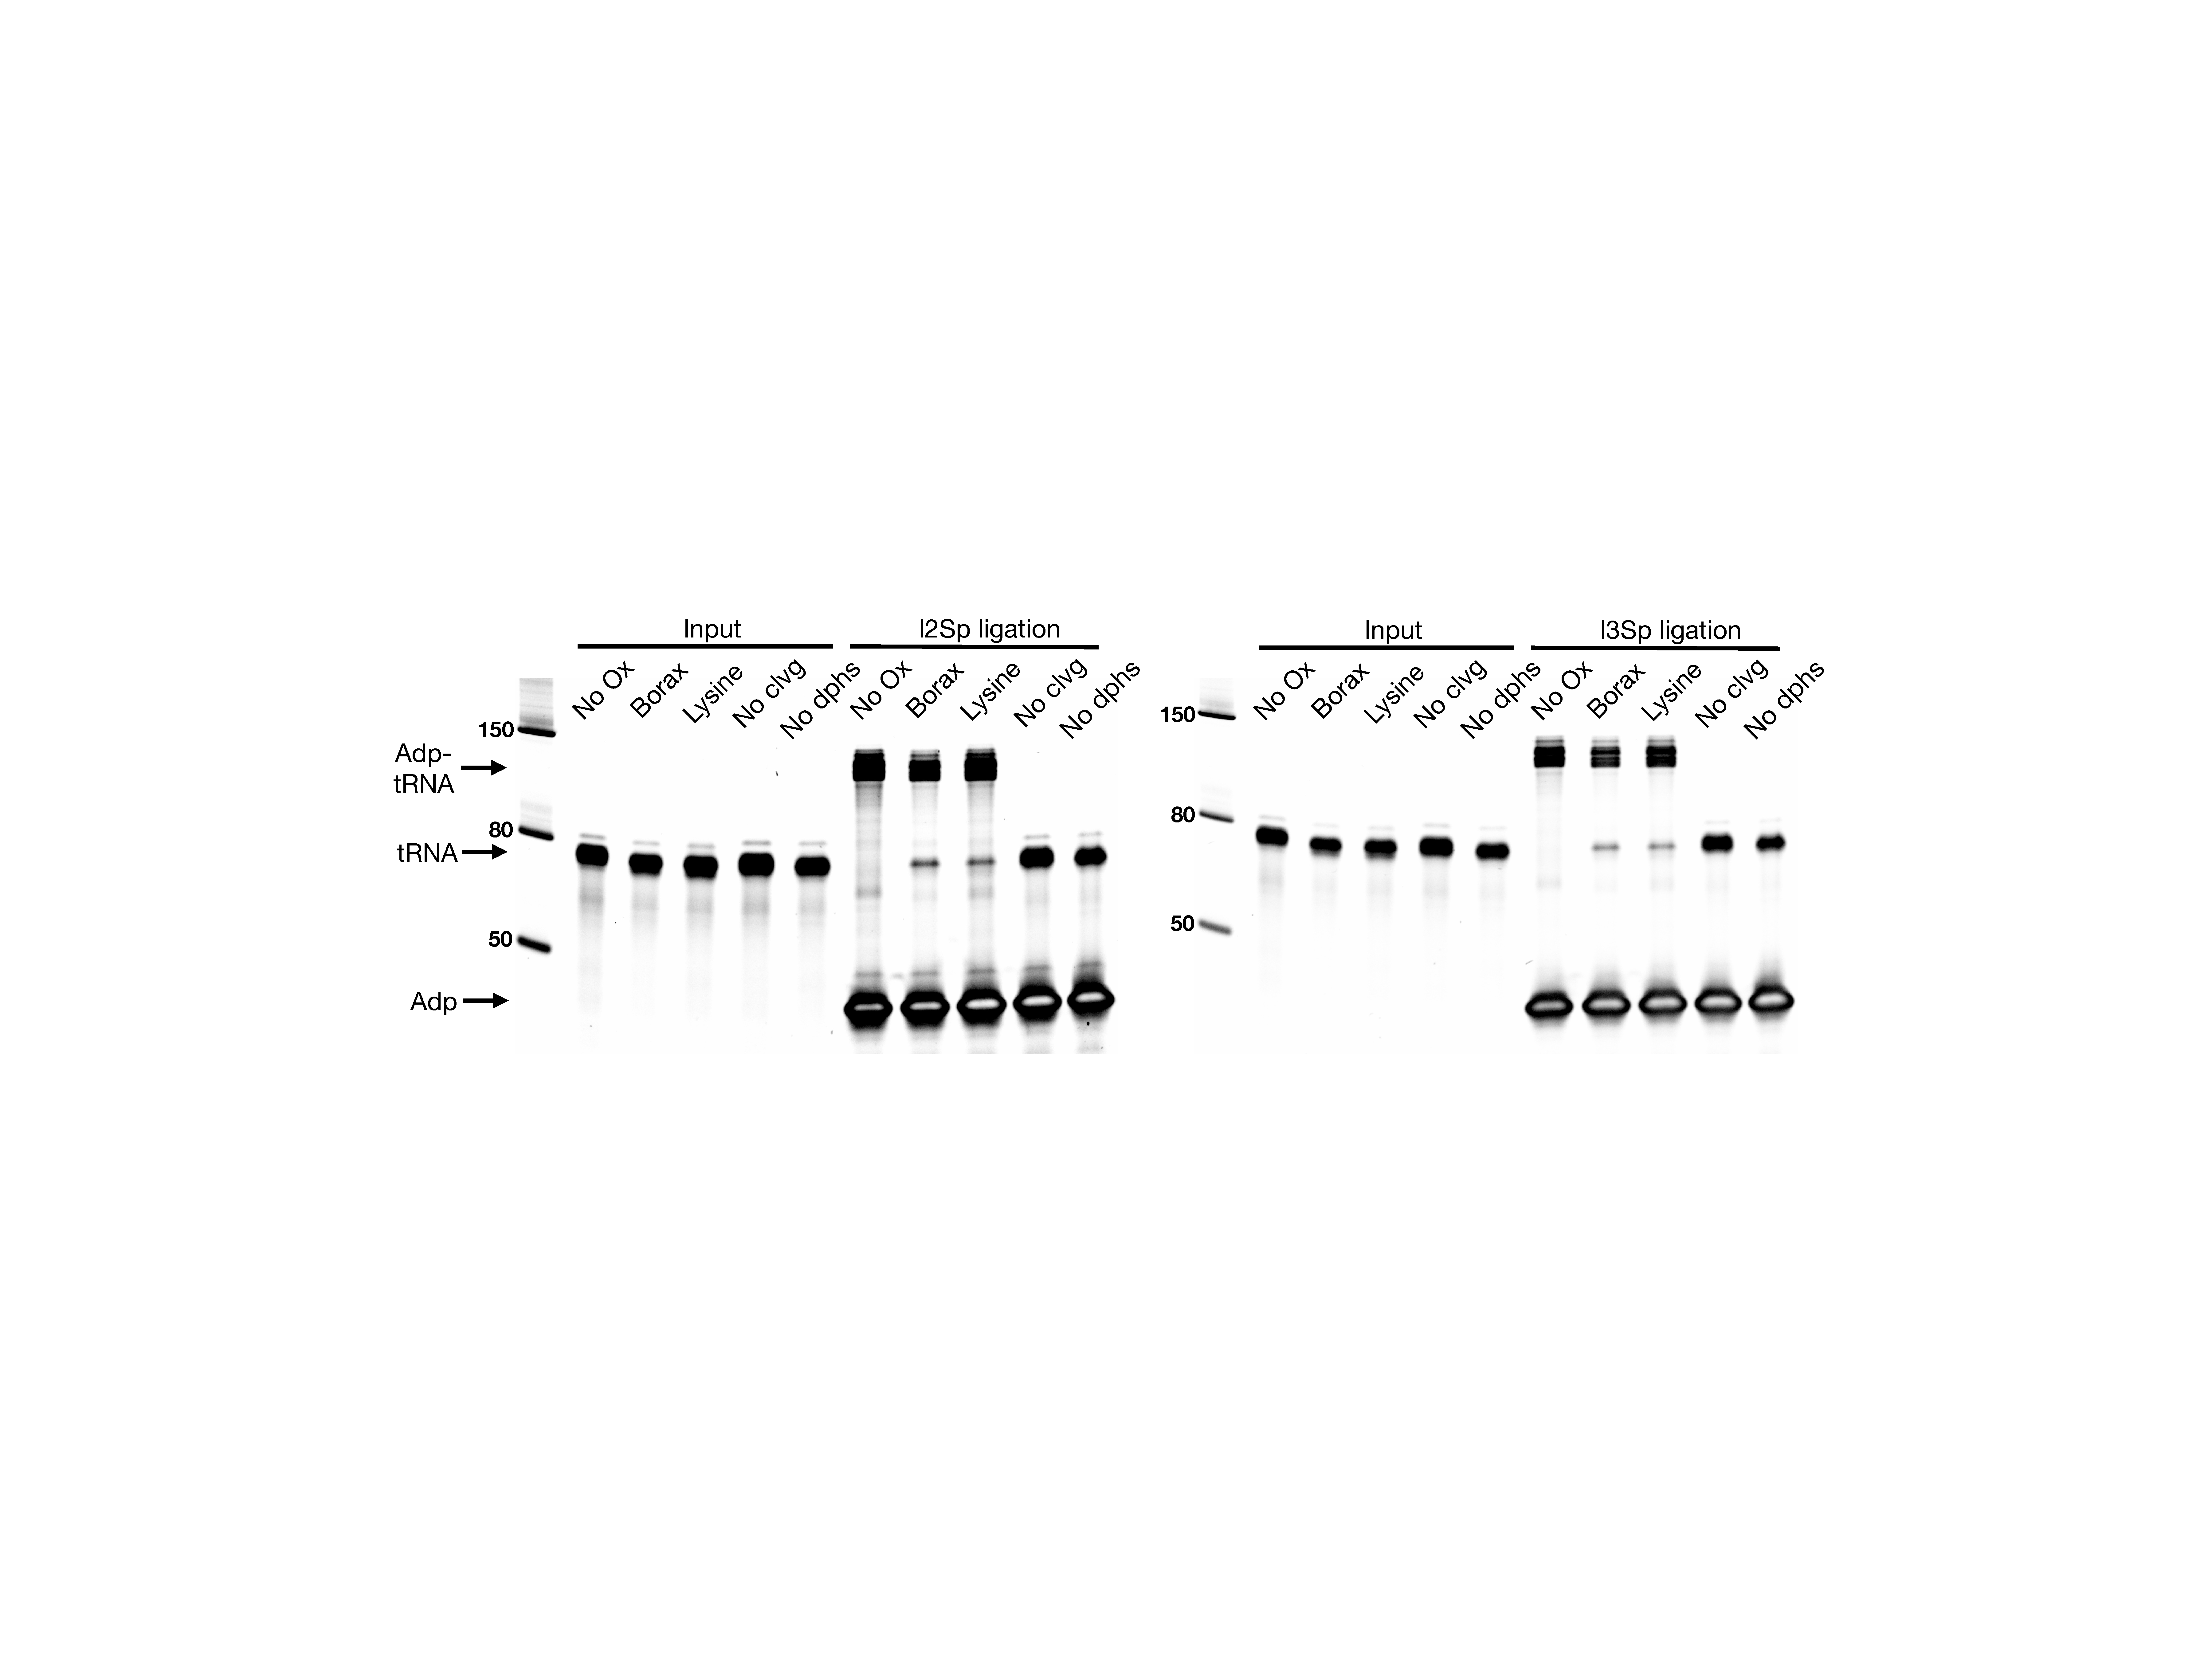
\includegraphics[width=0.85\linewidth]{figures/Fig2S5.pdf}}}\label{figsupp:f2S5}

\figsupp[Sequenced controls.]{
Charge tRNA-Seq control samples and spike-ins validate method.
\textbf{(A)} Cleavage of the 3′ adenosine on spike-in oligo is near complete.
Using the E.coli tRNA-Lys-CCA oligo as a spike-in control to monitor completion of the Whitfeld reaction.
If complete, 100\% E.coli tRNA-Lys-CC should be produced and thus appearing as 0\% charged.
\textbf{(B)} Aminoacylation level of tRNA transcripts after undergoing deacylation by incubation at 45°C for 4 h in 1 M lysine (pH=8).
Mitochondrial tRNA\textsuperscript{fMet} was excluded because formylated or acetylated amino acids are known to be highly resistant towards deacylation \citep{Schofield1968-qn}.
\textbf{(C)} Aminoacylation level of tRNA transcripts from four samples receiving sham oxidation (NaCl) during the Whitfeld reaction.
}{\fbox{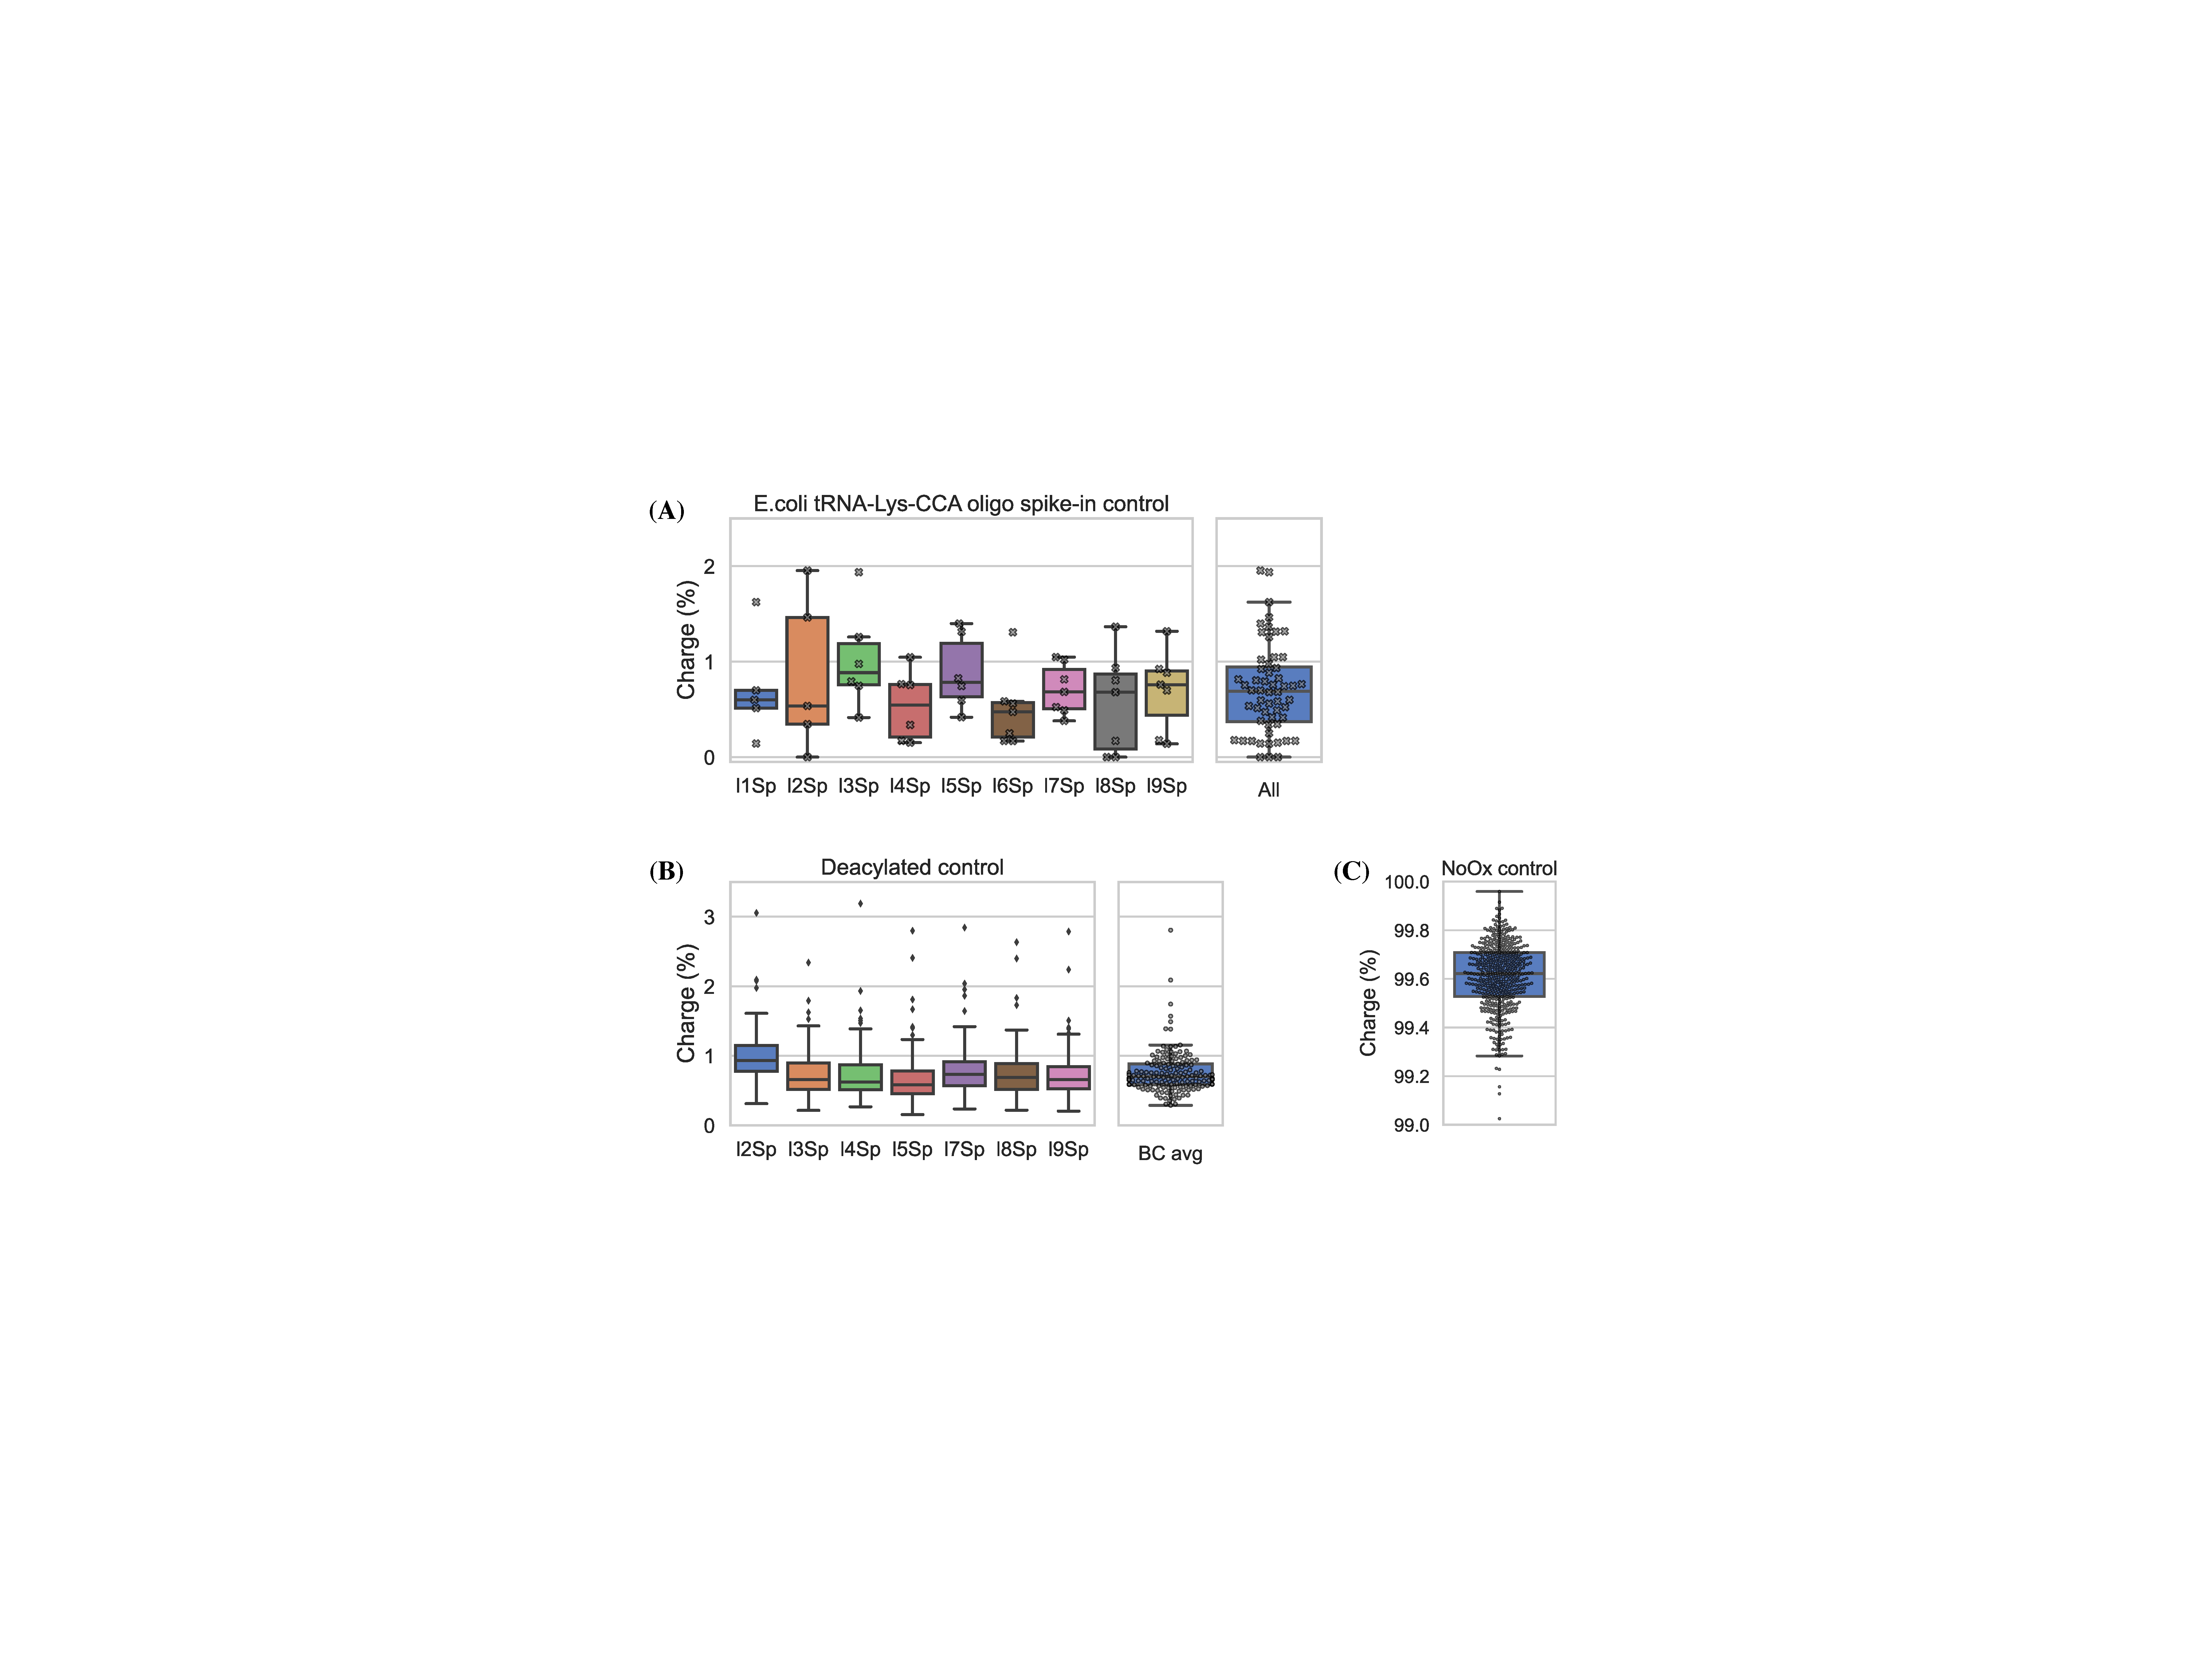
\includegraphics[width=0.7\linewidth]{figures/Fig2S6.pdf}}}\label{figsupp:f2S6}

\figsupp[RT readthrough comparing TGIRT to Maxima.]{
\textbf{(A)} The Maxima RT polymerase produces similar levels of full size cDNA as TGIRT-III under the standard (Std) tRNA-Seq RT-PCR conditions (42°C, 16 h, suggested by \cite{Behrens2021-gb}).
For Maxima, other incubation conditions tested are: 1 h at 60°C (similar to \cite{Lucas2023-vm}), 3 h at 60°C and 1 h at 60°C followed by 15 h at 42°C (1h+).
After RT-PCR, the RNA template was remove by NaOH hydrolysis, liberating the DNA adapter annotated on the gel.
\textbf{(B)} Coverage plots for cytoplasmic tRNA transcripts grouped by cognate amino acid, comparing samples prepared with TGIRT-III or Maxima using standard incubation (42°C, 16 h).
\textbf{(C)} Percentage of full length transcripts grouped by cognate amino acid (i.e. left side of plots in panel B).
Errorbars are bootstrapped 95\% confidence interval of the mean over the 7 individual samples barcoded, pooled and used for RT-PCR template with both TGIRT-III and Maxima.
}{\fbox{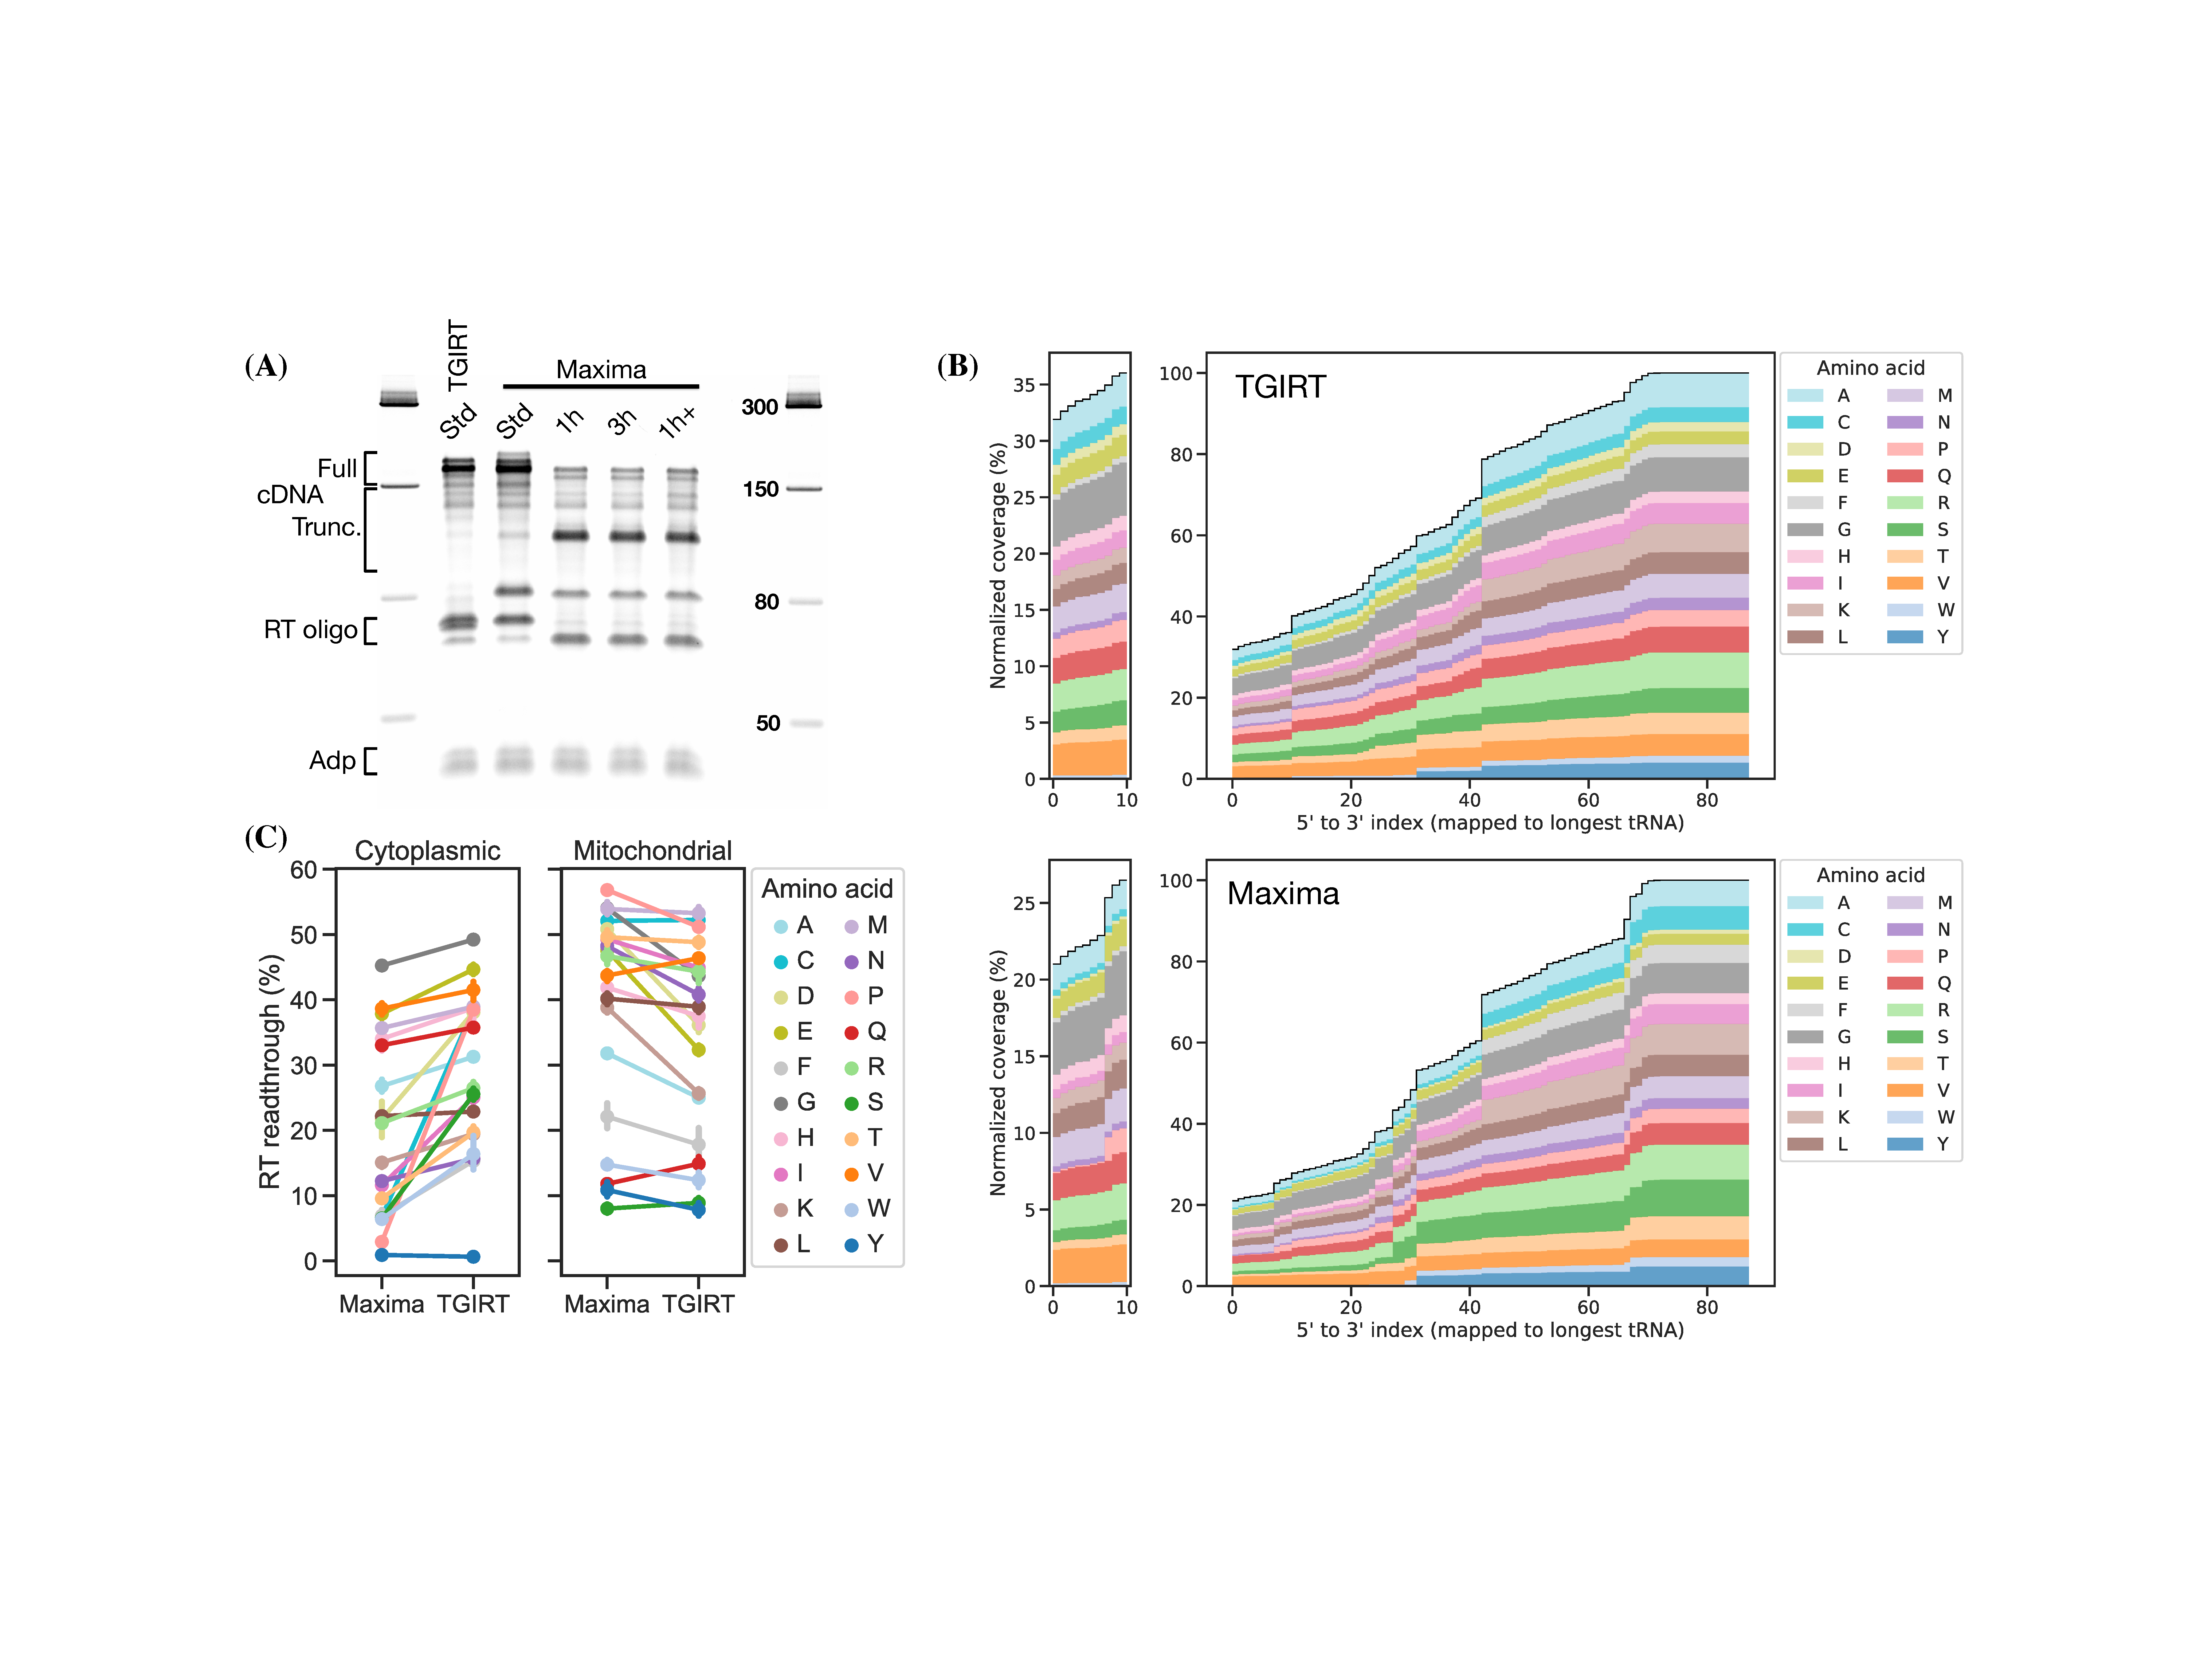
\includegraphics[width=0.85\linewidth]{figures/Fig2S7.pdf}}}\label{figsupp:f2S7}

\figsupp[tRNA homology requires careful PCR conditions.]{
\textbf{(A)} The specificity of the final library PCR step (attaching Illumina P7 and P5 sequences) deteriorates with increasing product-to-primer ratios, probably due to high tRNA homology and PCR crossover \citep{Holcomb2014-vz}.
\textbf{(B)} tRNA-Seq DNA library reannealing is inhibited by high salt concentrations.
A gel purified charge tRNA-Seq DNA library was resuspended in TBE buffer and incubated 30 min at different temperatures with or without 1 M NaCl.
}{\fbox{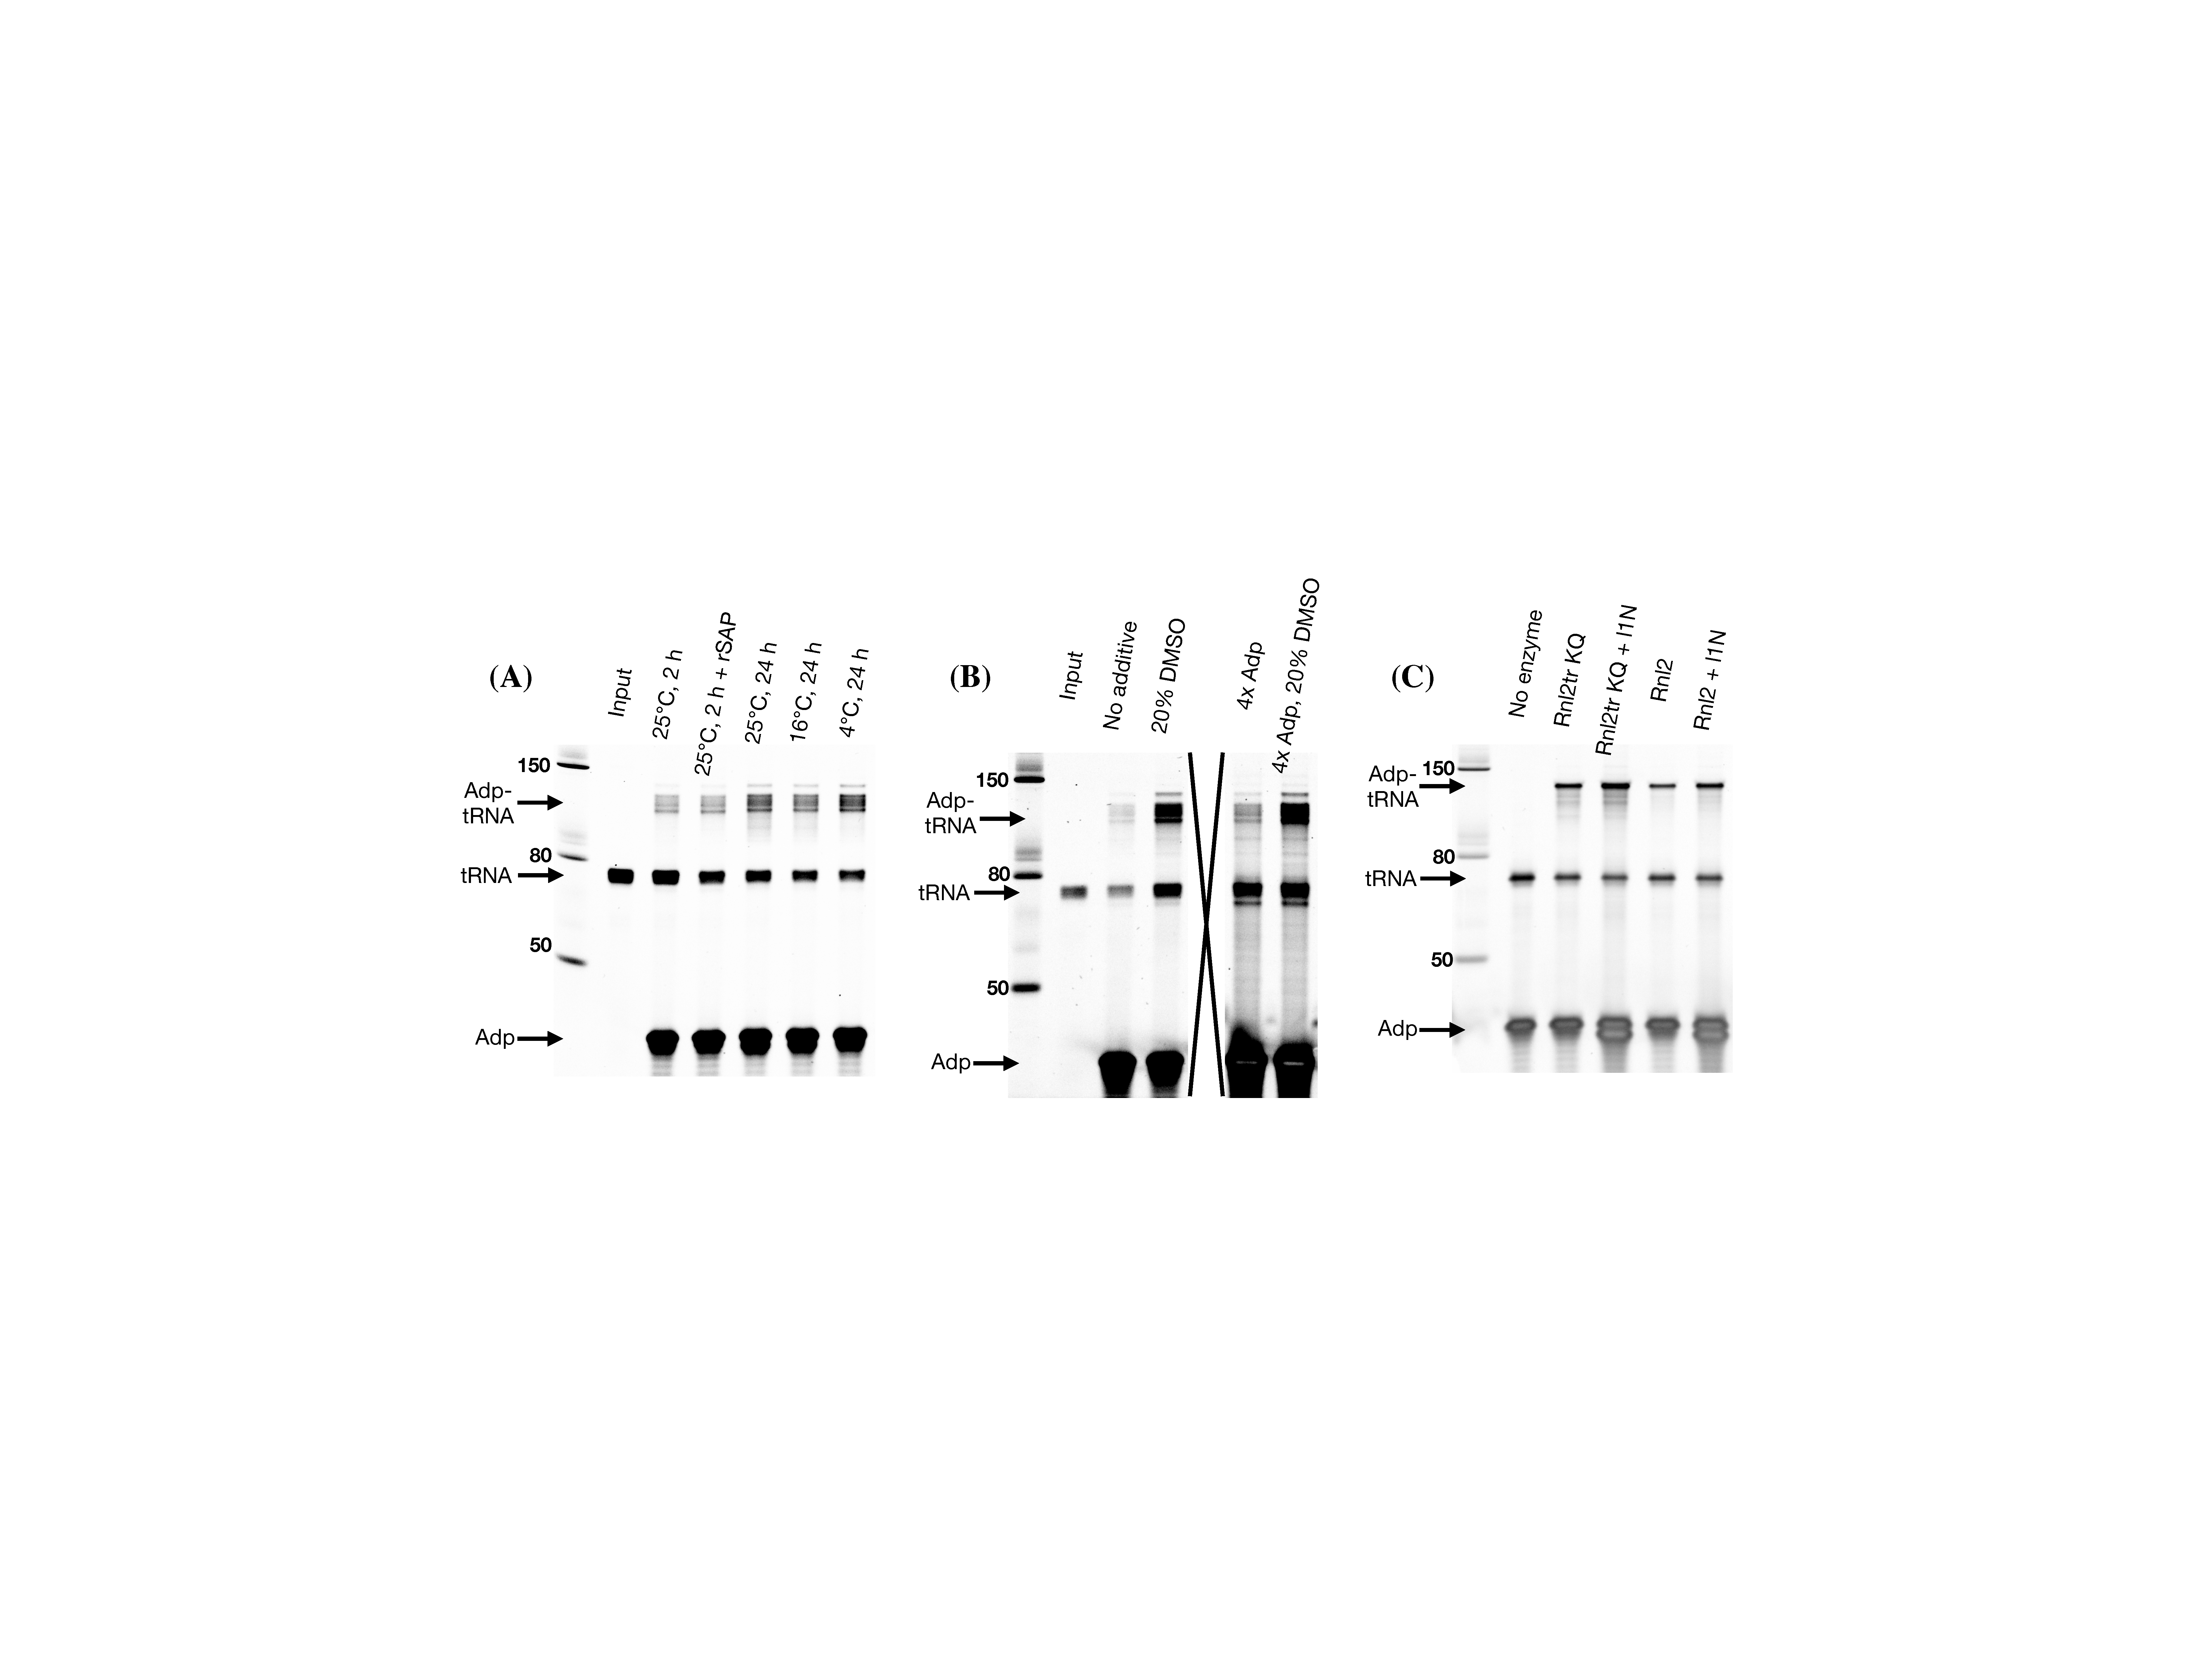
\includegraphics[width=0.5\linewidth]{figures/Fig2S8.pdf}}}\label{figsupp:f2S8}

\end{figure}




\subsection{Reference masking improves read mapping}
It has previously been noted that alignment of tRNA reads is challenging due to RT misincorporations and falloff \citep{Hoffmann2018-uz, Behrens2021-gb}.
Most commonly, the Bowtie1 or Bowtie2 aligners have been applied using various settings to accommodate short reads and the many mismatches \citep{Cozen2015-cx, Zheng2015-kj, Clark2016-ph, Evans2017-st, Pinkard2020-yd}.
However, although these are ultra-fast, Bowtie1 does not support alignments with insertions or deletions, and while Bowtie2 does, neither can guarantee that the best alignment is returned \citep{Langmead2009-yx, Langmead2012-ui}.
We reasoned that many users of tRNA-Seq would rather sacrifice computational speed over mapping accuracy and therefore we apply a full all-against-all local alignment using the Smith-Waterman algorithm to provide the guaranteed best alignment(s).
This is possible because the set of tRNA transcripts in a reference is only a few hundred sequences and thus we are able to align 1e8 tRNA-Seq reads to a human tRNA reference with 282 sequences in XXX h on a YYYY [number of cores, clock speed].

In addition to the choice of read alignment method, \cite{Behrens2021-gb} found that using a SNP-tolerant alignment substantially improved mapping when modified positions were defined as SNPs.
We adapted this approach by masking modified positions in the reference to "N"; however, we cannot rely on annotated modifications because these are incomplete and their effect on RT misincorporation rates is hard to predict.
Instead, we used the misincorporation information embedded in the sequencing data, extracting it after a first pass alignment and then using mismatch frequencies for reference masking.
As such, this is an iterative process because the alignment will change slightly with a new masked reference.
In addition to the number of iterations, masking is only applied on positions with a minimum mismatch frequency (\verb|min_mut_freq|) and either including or excluding reads with multiple transcript alignments (\verb|unique_anno_float|).
Furthermore, a parameter (\verb|frac_max_score|) controls the sharing of a mask to  highly similar transcripts.
To find the optimal combination of parameters for reference masking we performed a grid search with the objective of finding the masking that resulted in the least number of reads assigned to transcripts with multiple codons (\FIG{Fig3}, panel A).
This lead to 334 positions in the 282 sequence reference getting masked and resulting in an alignment improvement from 11.34\% to 4.37\% reads with multiple codon alignments.

Masked positions do not contribute to the alignment score and thus possibly lowering it below the minimum threshold; however, we observed no trade-off between optimized reference masking and read mapping percentage (\FIG{Fig3}, panel B).
Like \cite{Behrens2021-gb}, we observe a striking difference in the mapping of certain tRNA transcripts.
For example, transcripts decoding the Ser-UCU codon (AGA anticodon) are lifted out of obscurity (\FIG{Fig3}, panel C).
Generally, reference masking appears to increase annotations for around a dusin transcripts but a substantial mapping change only occurs for four codons (\FIGSUPP[Fig3]{f3S1}, panel a).
The effect of reference masking on the charge measurements was low as expected because this is a relative number (\FIGSUPP[Fig3]{f3S1}, panel B).





\subsubsection{tRNA modifications are reflected in mismatches, gaps and RT stops}
Our computational method also supports using misincorporation data for inference of nucleotide modifications which is typically only valid for modifications that disrupt Watson–Crick base pairing such as methylations \citep{Clark2016-ph, Behrens2021-gb}.
As such the 5-methoxycarbonylmethyl-2-thiouridine (mcm5s2U) modification should be silent; however, thionucleosides are sensitive to periodate treatment, oxidizing them to sulfonates and making them further sensitive to nucleophilic attack \citep{Ziff1968-la, Rao1974-zq}.
When periodate oxidation of mcm5s2U is followed by lysine cleavage it would presumably result in a lysine adduct \citep{Ziff1968-la}, thus disrupting Watson–Crick base pairing.
We verified this by comparing the misincorporation signature in samples processed with/without periodate oxidation, focusing on the human tRNAs Lys-UUU, Gln-UUG, Glu-UUC and Arg-UCU shown by \cite{Lentini2018-xs} to carry be mcm5s2U modification (\FIGSUPP[Fig3]{f3S2}).
Large changes in the misincorporation signature is observed upon periodate oxidation, but curiously some tRNAs respond with a large decrease in RT readthrough while others see an increase in the mutation and/or gap frequency.
Similar observations were recently showed by \cite{Katanski2022-ij}.

\begin{figure}[ht!]
\centering
\fbox{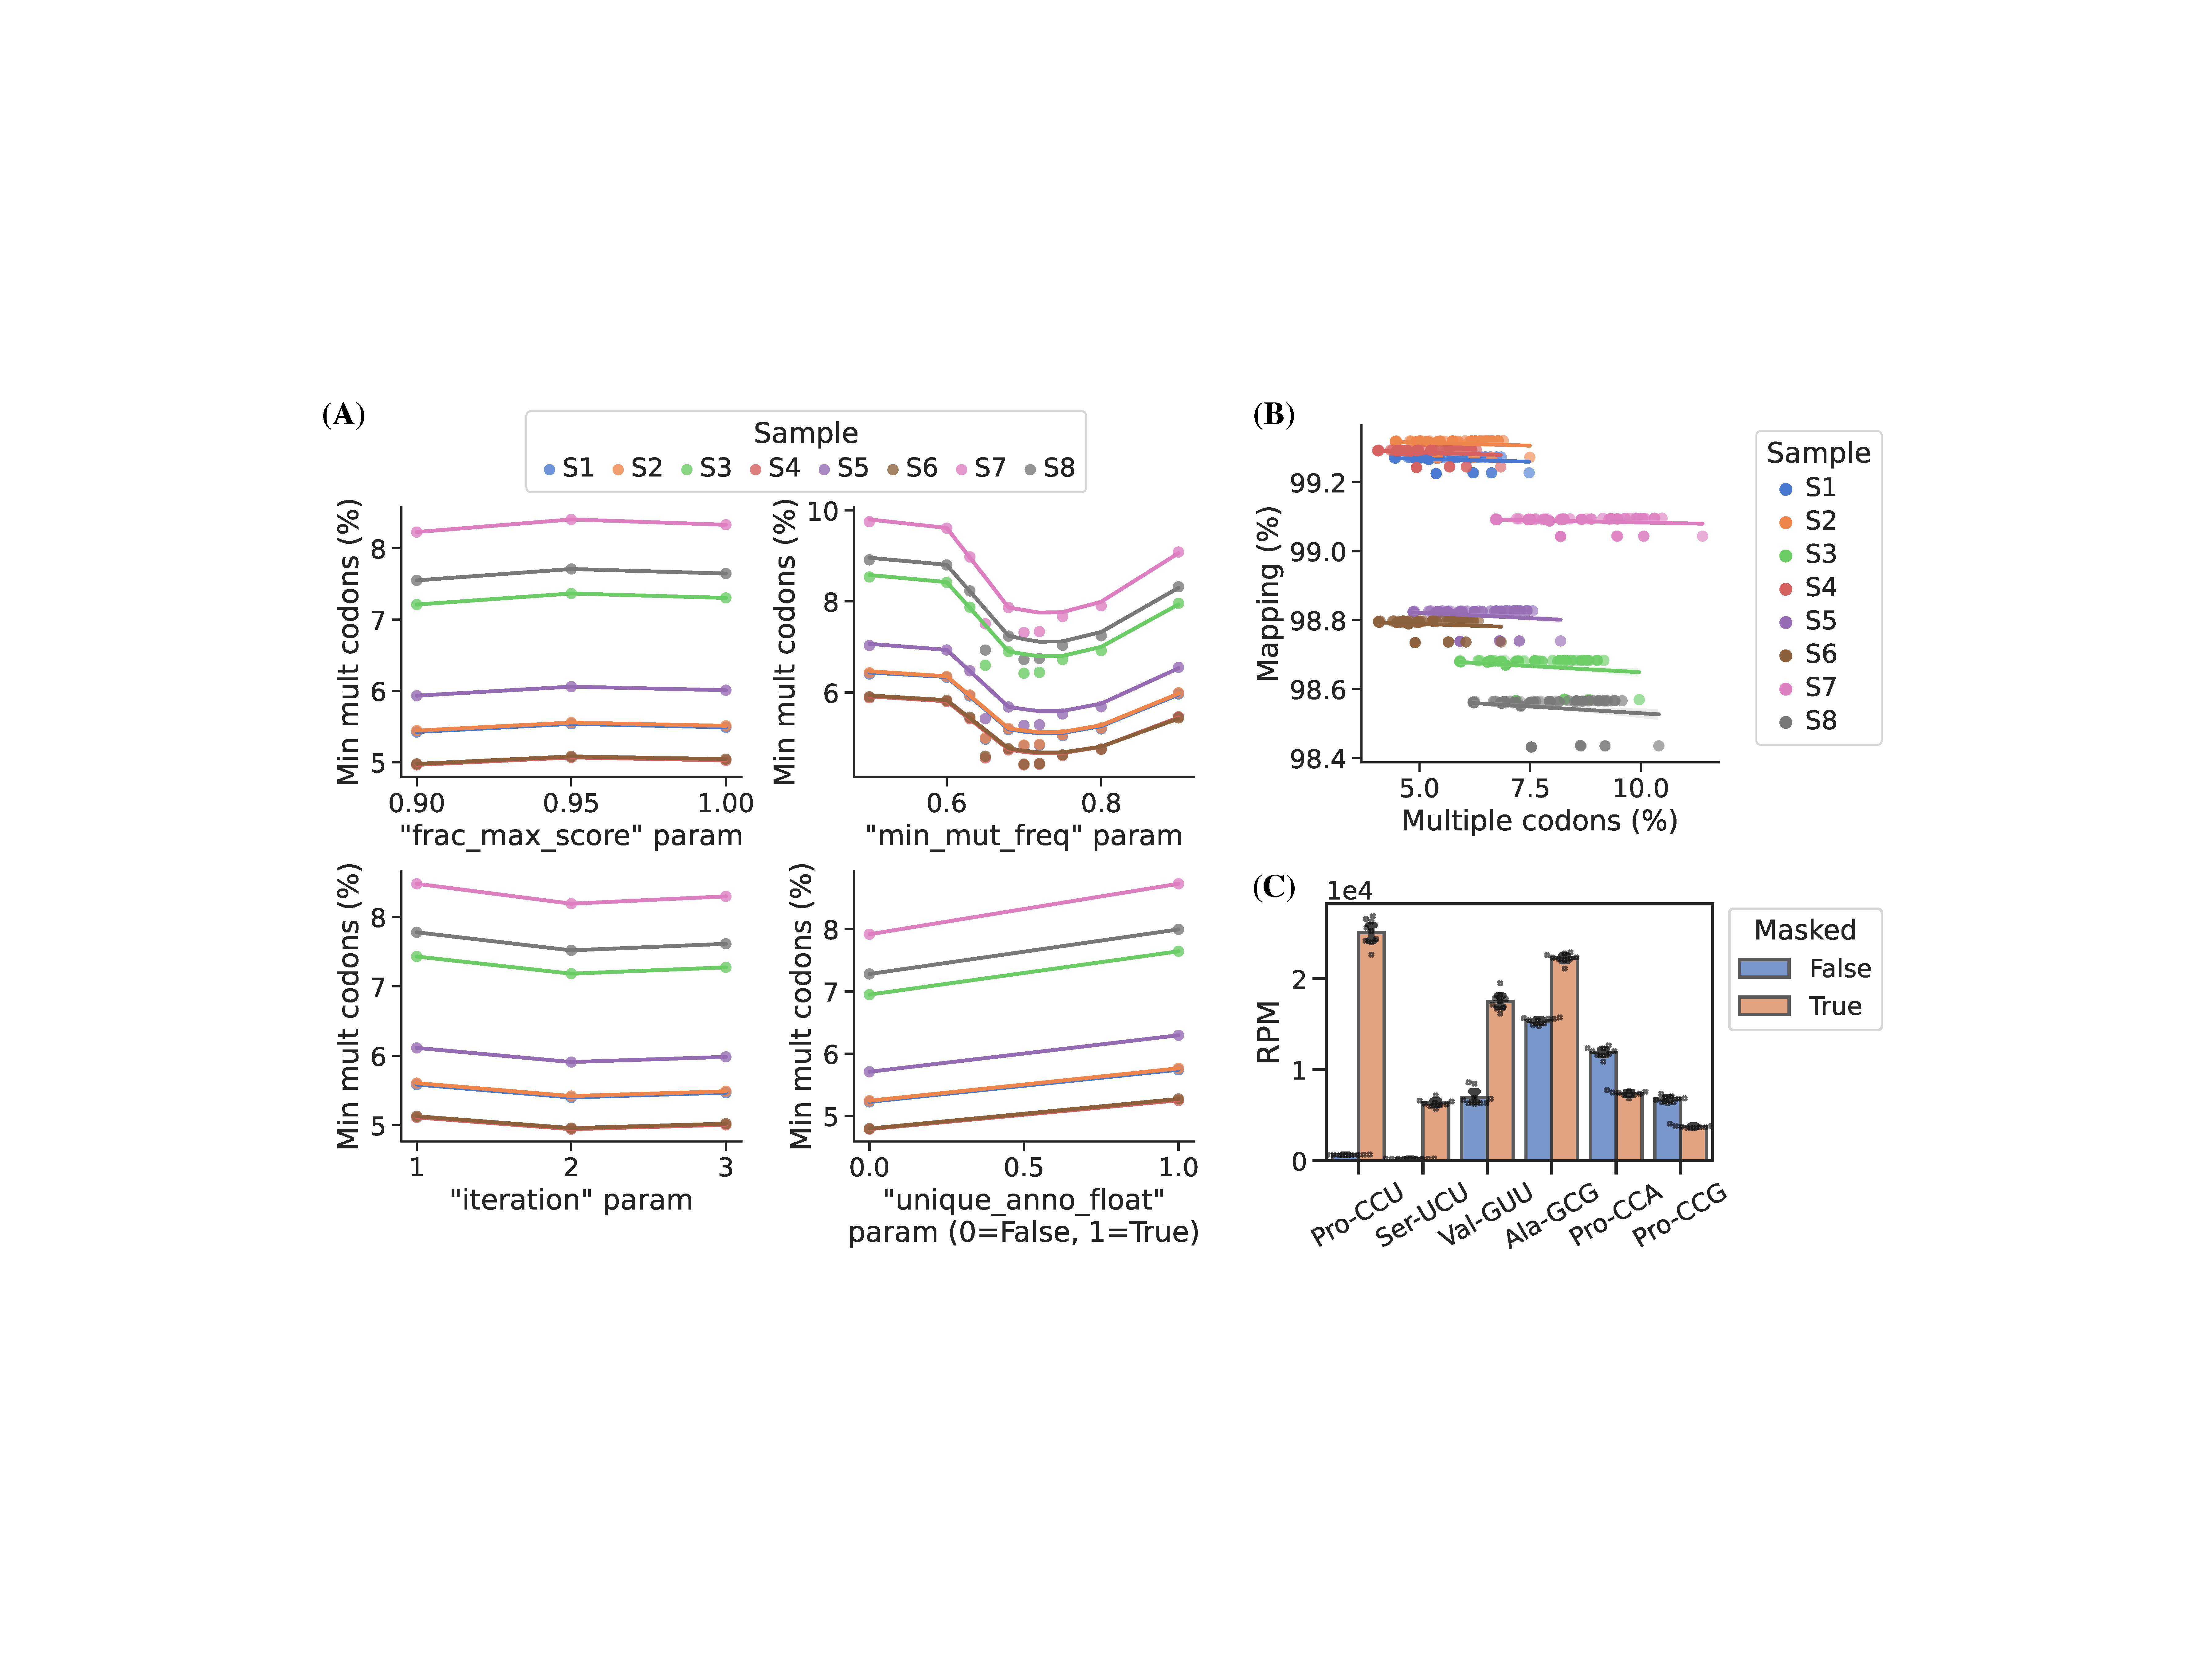
\includegraphics[width=0.85\linewidth]{figures/Fig3.pdf}}
\caption{
Masking of reference tRNA transcript sequences improves alignment performance.
\textbf{(A)} Grid search optimization of parameters determining the extent of reference masking (see method section for details).
Each subplot shows the effect of one tuning parameter when combined with the best combination of the other three.
Parameters used for reference masking are chosen to minimize the percentage of reads assigned to tRNAs with multiple codons.
\textbf{(B)} There is no trade-off between mapping success and multiple codon mapping.
\textbf{(C)} Reference masking increase RPM values of select codons.
RPM levels of the codons shown was found before and after optimized reference masking.
Errorbars are bootstrapped 95\% confidence interval of the mean over the 9  barcode replicate samples.
}
\label{fig:Fig3}

\figsupp[Reference masking effect on RPM and charge levels.]{
\textbf{(A)} Reference masking effect on RPM levels per transcripts (left) and per codon (right).
Transcript points showing $>3$, and codon points showing $>1.5$, fold increase or decrease upon reference masking are colored orange.
The highest fold change transcripts and codons are annotated on the right side of the plot.
\textbf{(B)} Reference masking effect on charge levels per transcripts (left) and per codon (right).
Points showing $>1.05$ fold increase or decrease upon reference masking are colored orange and annotated on the right side of the plot.
}{\fbox{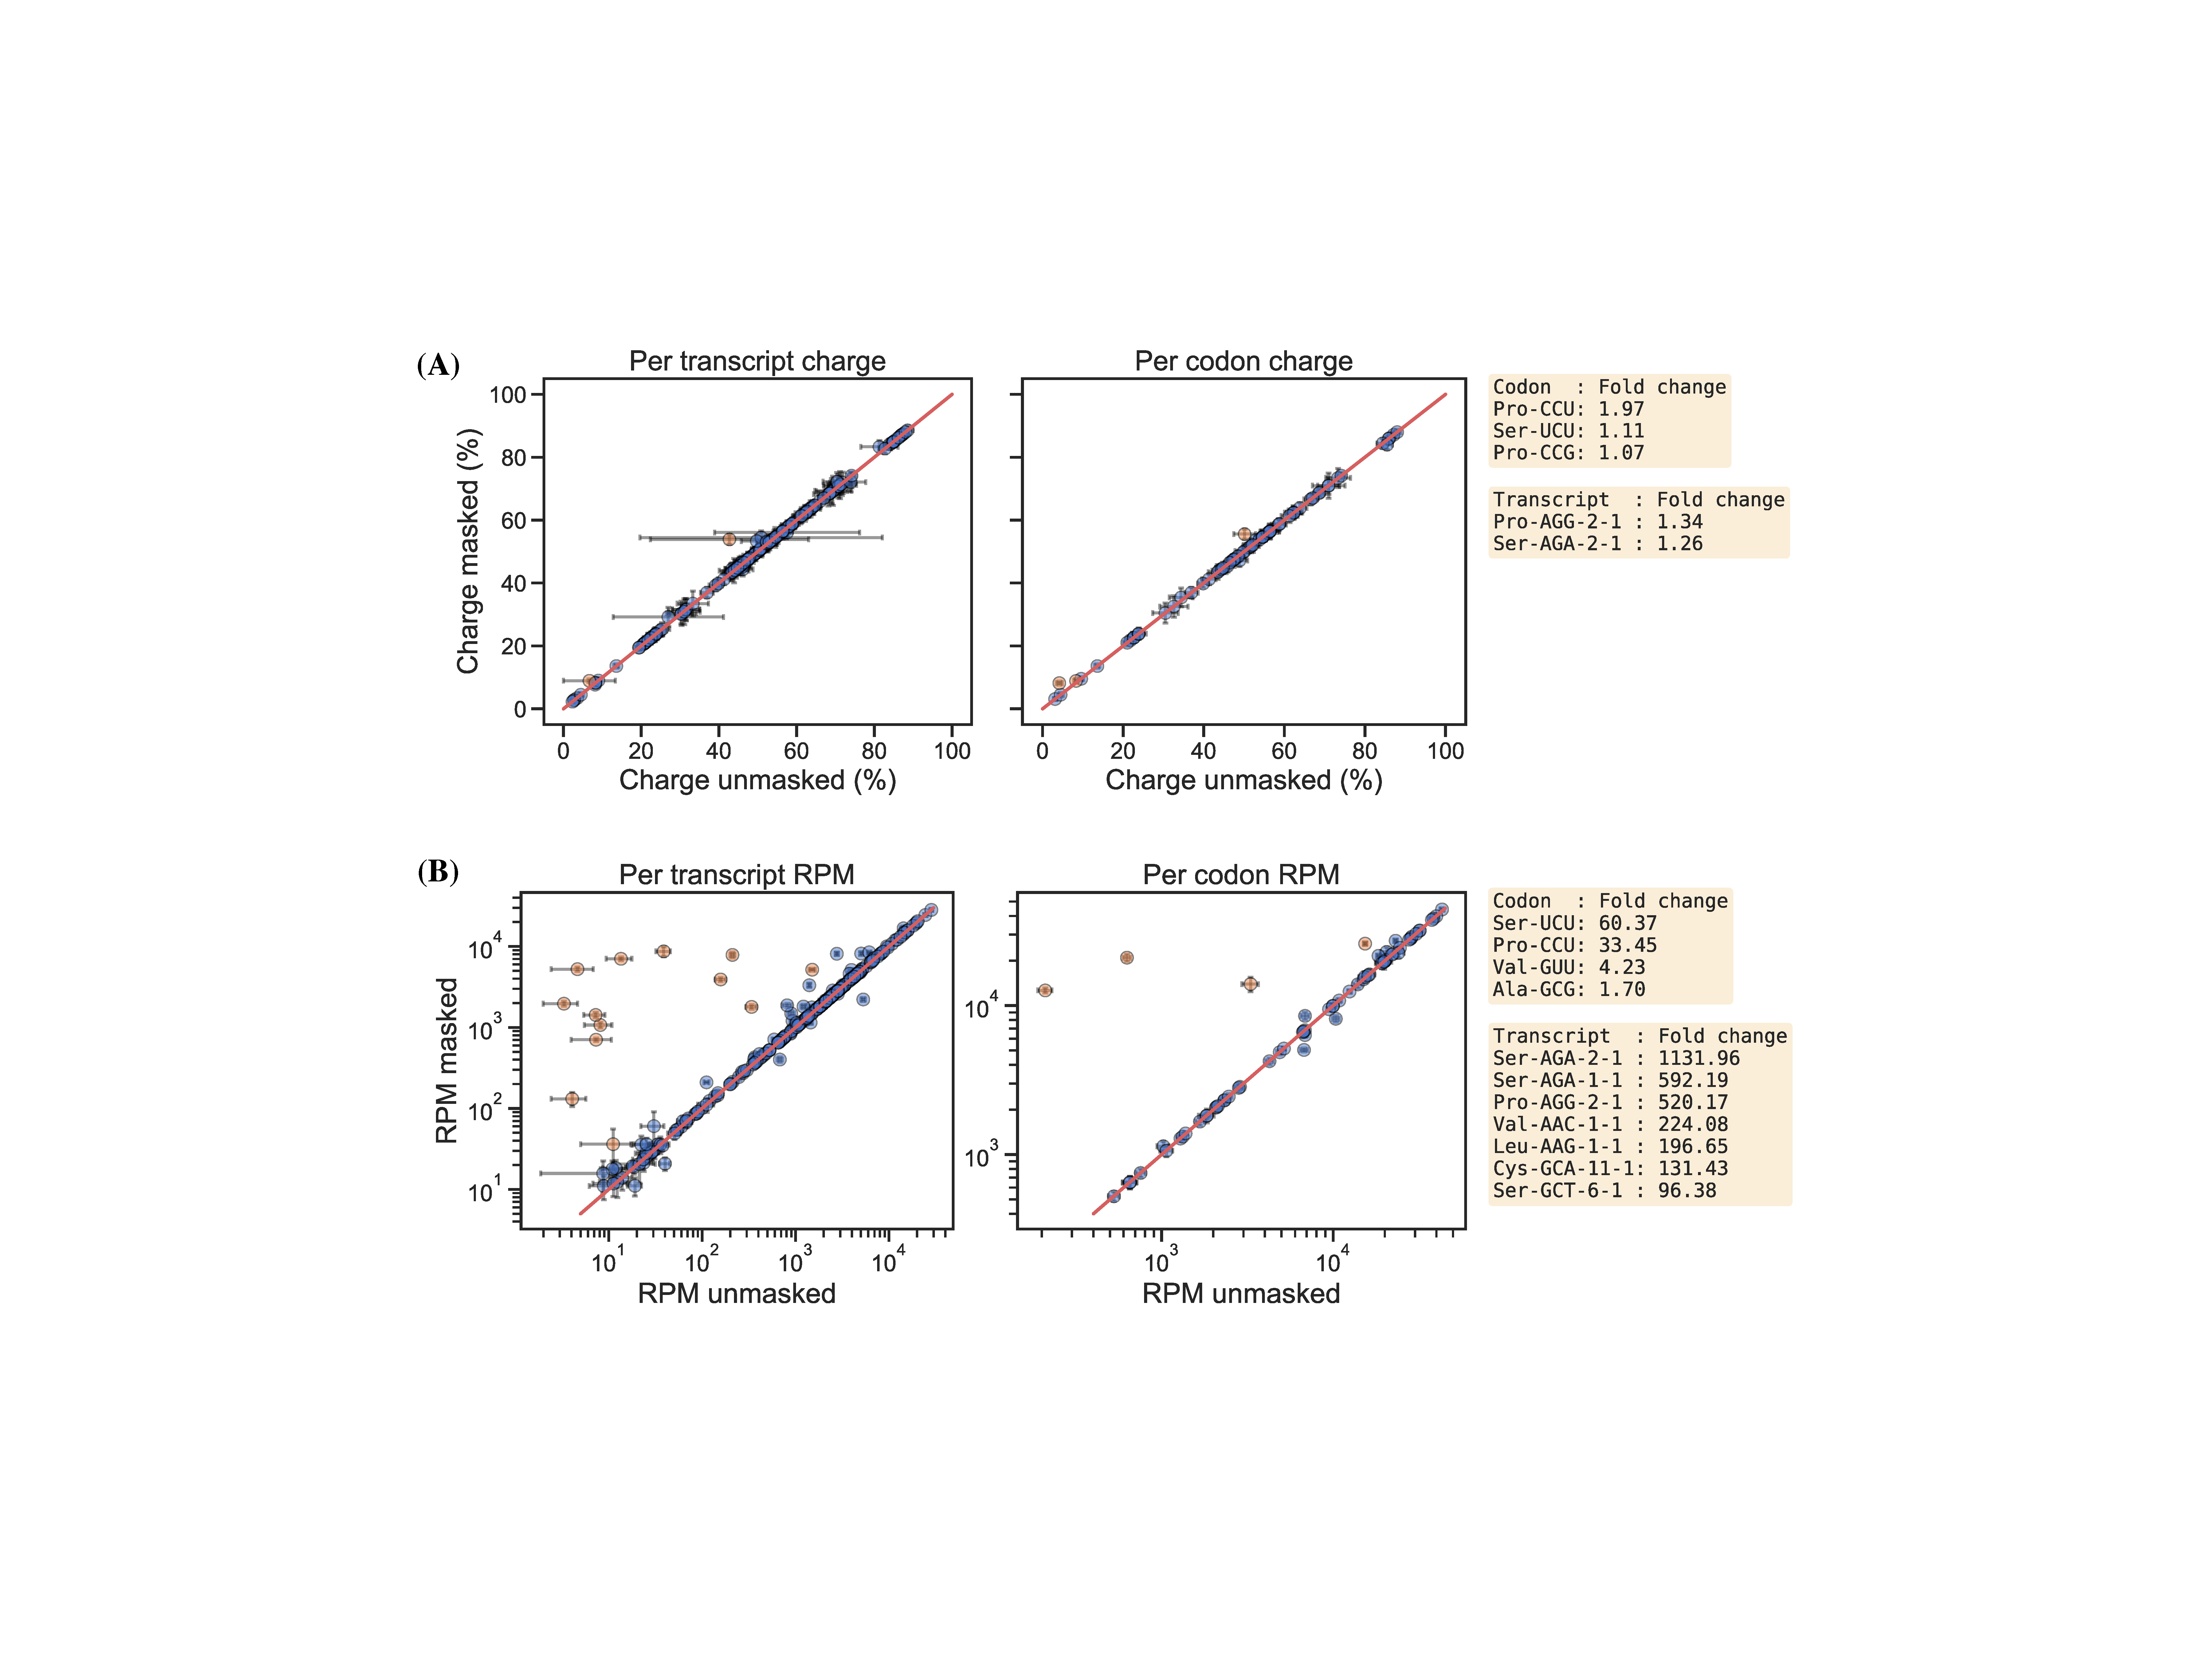
\includegraphics[width=0.85\linewidth]{figures/Fig3S1.pdf}}}\label{figsupp:f3S1}

\figsupp[Anticodon modification mcm5s2U is detected in periodate oxidized samples.]{
Mismatch frequency, gap frequency and RT stop percentage is increased upon periodate oxidation for transcripts known to be 5-methoxycarbonylmethyl-2-thiouridine (mcm5s2U) modified.
The mcm5s2U modification has been shown to be present on the first anticodon nucleoside (position 34) in human tRNA Lys-UUU, Gln-UUG, Glu-UUC and Arg-UCU, while absent in the similar tRNA Arg-UCG \citep{Lentini2018-xs}.
}{\fbox{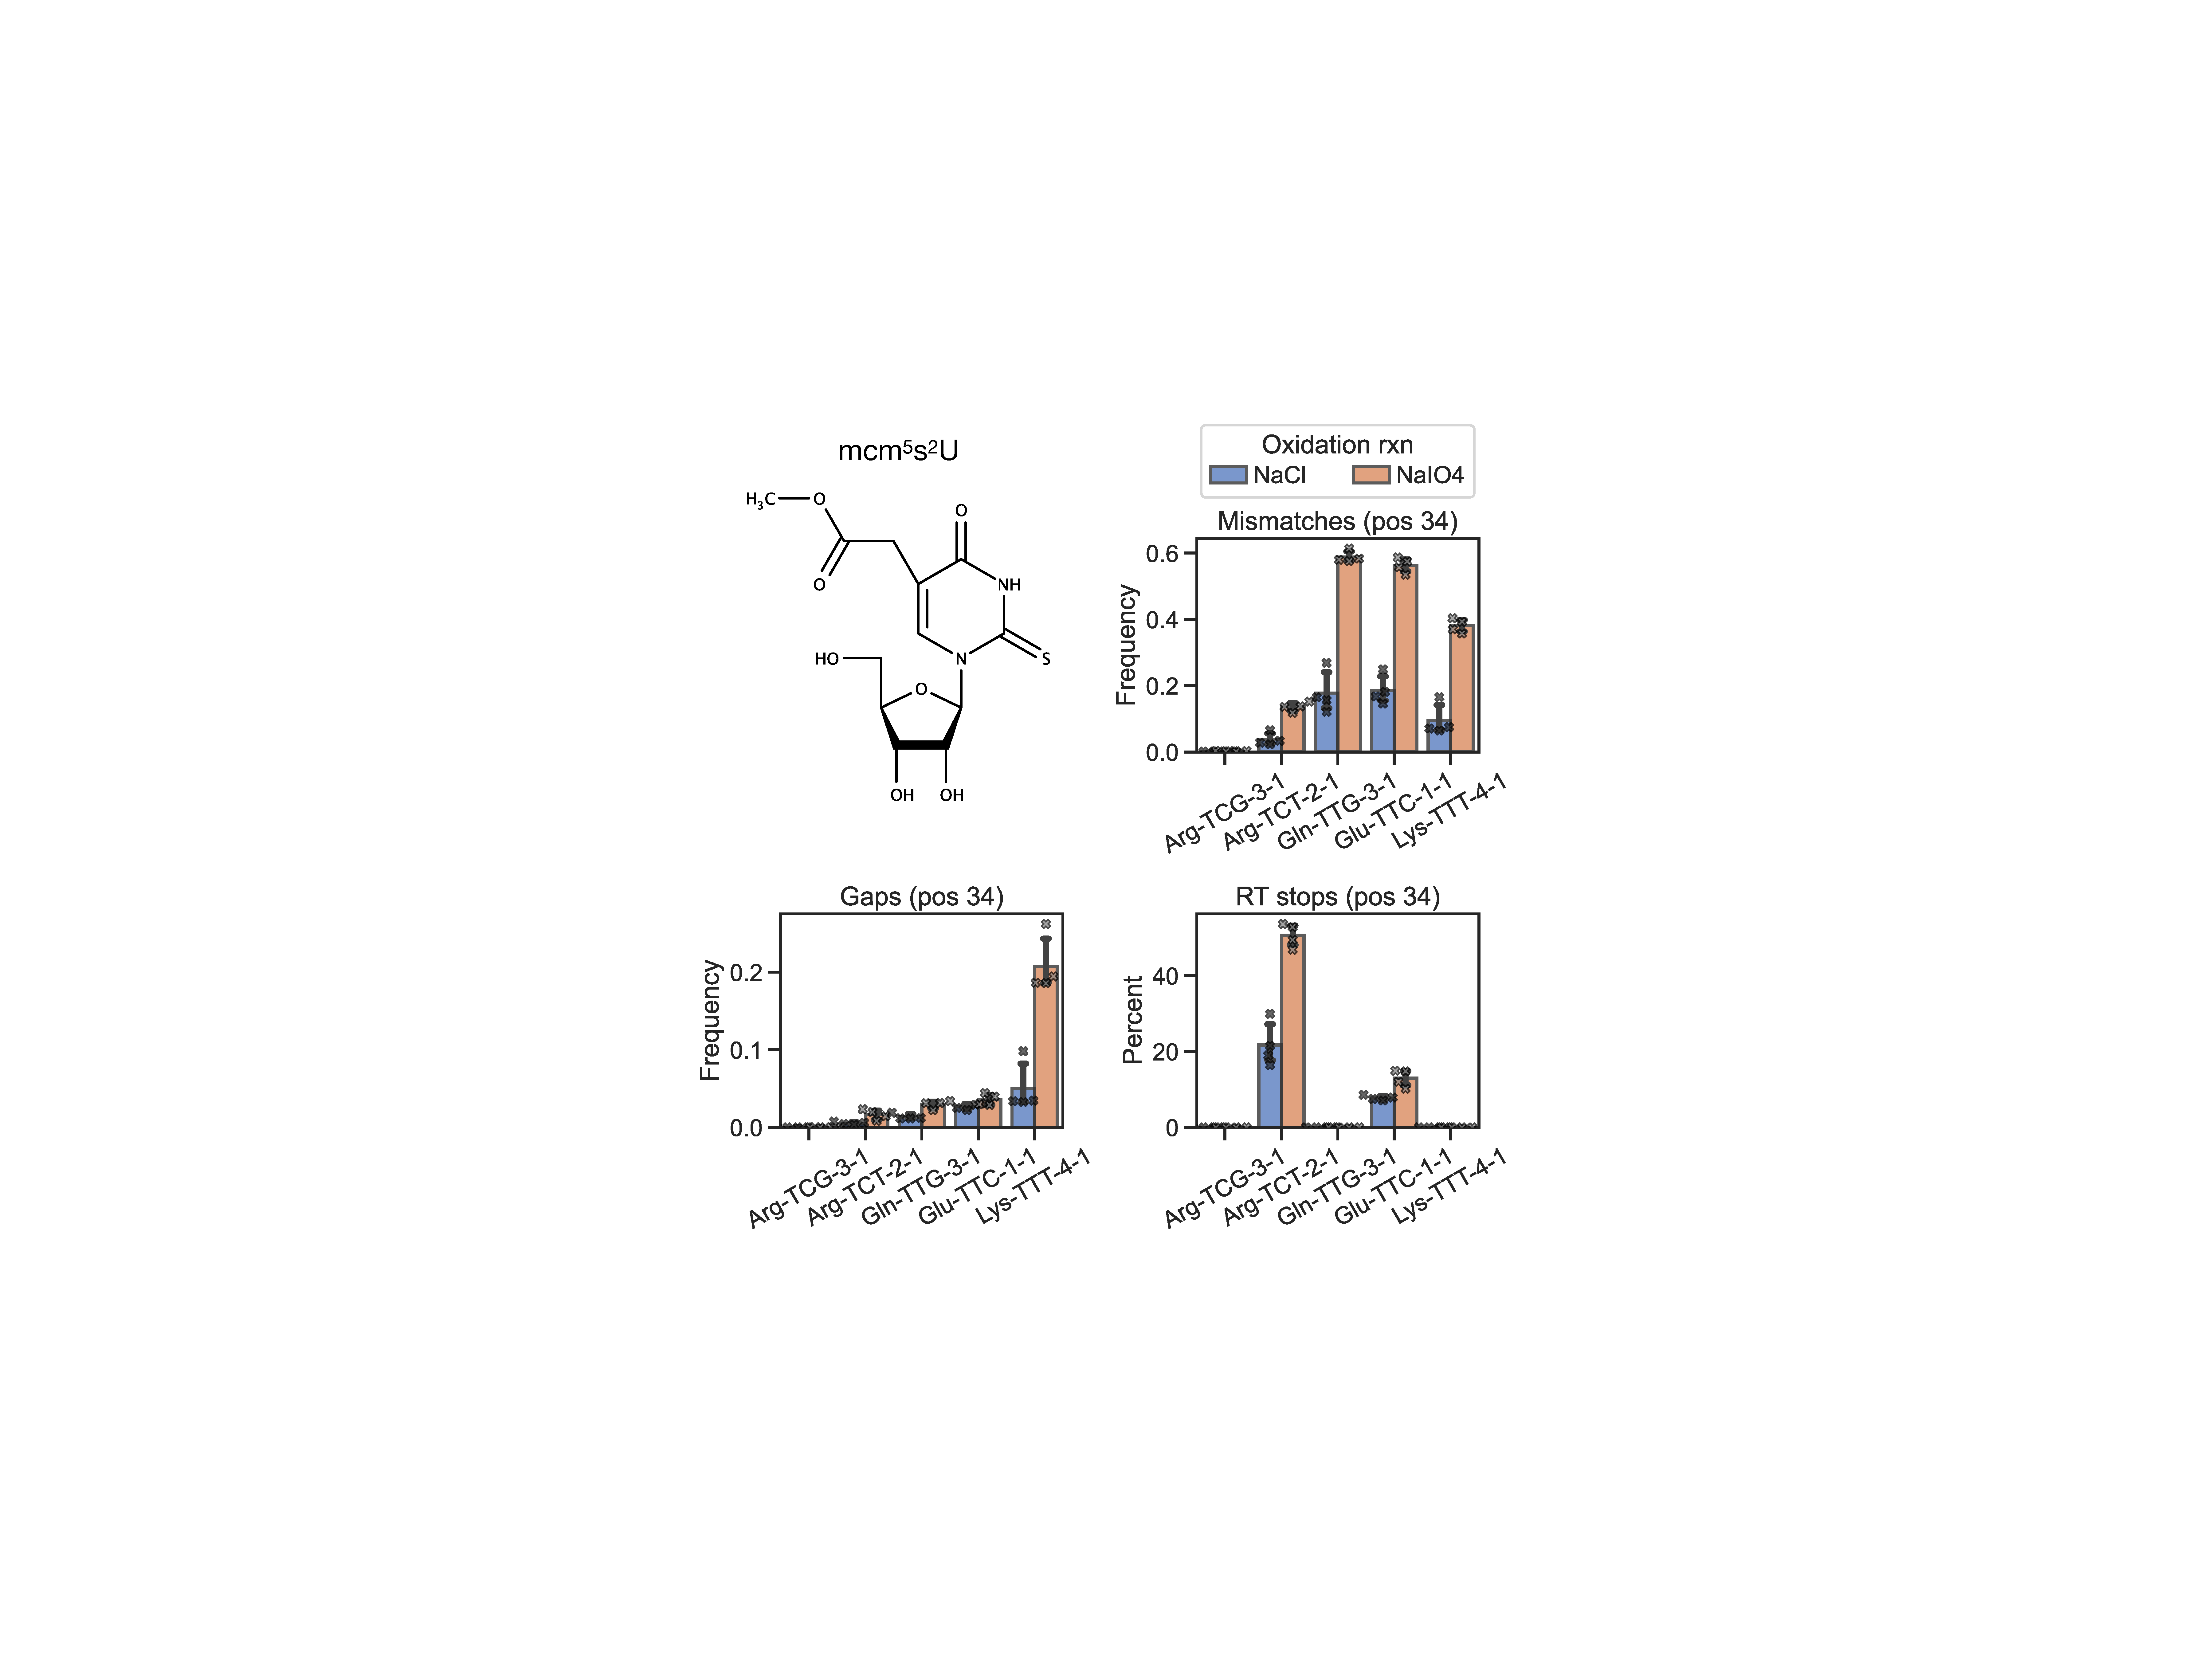
\includegraphics[width=0.55\linewidth]{figures/Fig3S2.pdf}}}\label{figsupp:f3S2}
\end{figure}





\subsection{Barcode replicates show high precision}
To assess our measurement precision, we performed our charge tRNA-Seq protocol on the same tRNA sample using all nine barcoded adapters.
We used partially deacylated RNA to achieve a representative spread of aminoacylation levels within a single sample (\FIGSUPP[Fig4]{f4S2}, panel A) and then extracted differences compared to the median barcode replicate measurement.
When comparing charge measurements binned by barcode, we observed that most were narrowly distributed with the median close to zero indicating little or no barcode bias (\FIG{Fig4}, panel A).
Adapter l4Sp is the exception that proves why barcode bias needs to be investigated, because it is consistently overestimating charge levels, with a median overestimate of $\sim$3 percentage points.
Overall however, charge measurements show high precision with a standard deviation from the median of just 1.7 percentage points, with similar results at the transcript level (\FIGSUPP[Fig4]{f4S1}, panel A).

For RPM values, some barcode replicates were more narrowly distributed than others. However, these differences are small and with a standard deviation from the median of 5.1 percentage we consider the RPM measurements to be precise (\FIG{Fig4}, panel B and \FIGSUPP[Fig4]{f4S1}, panel B).

\begin{figure}[ht!]
\centering
\fbox{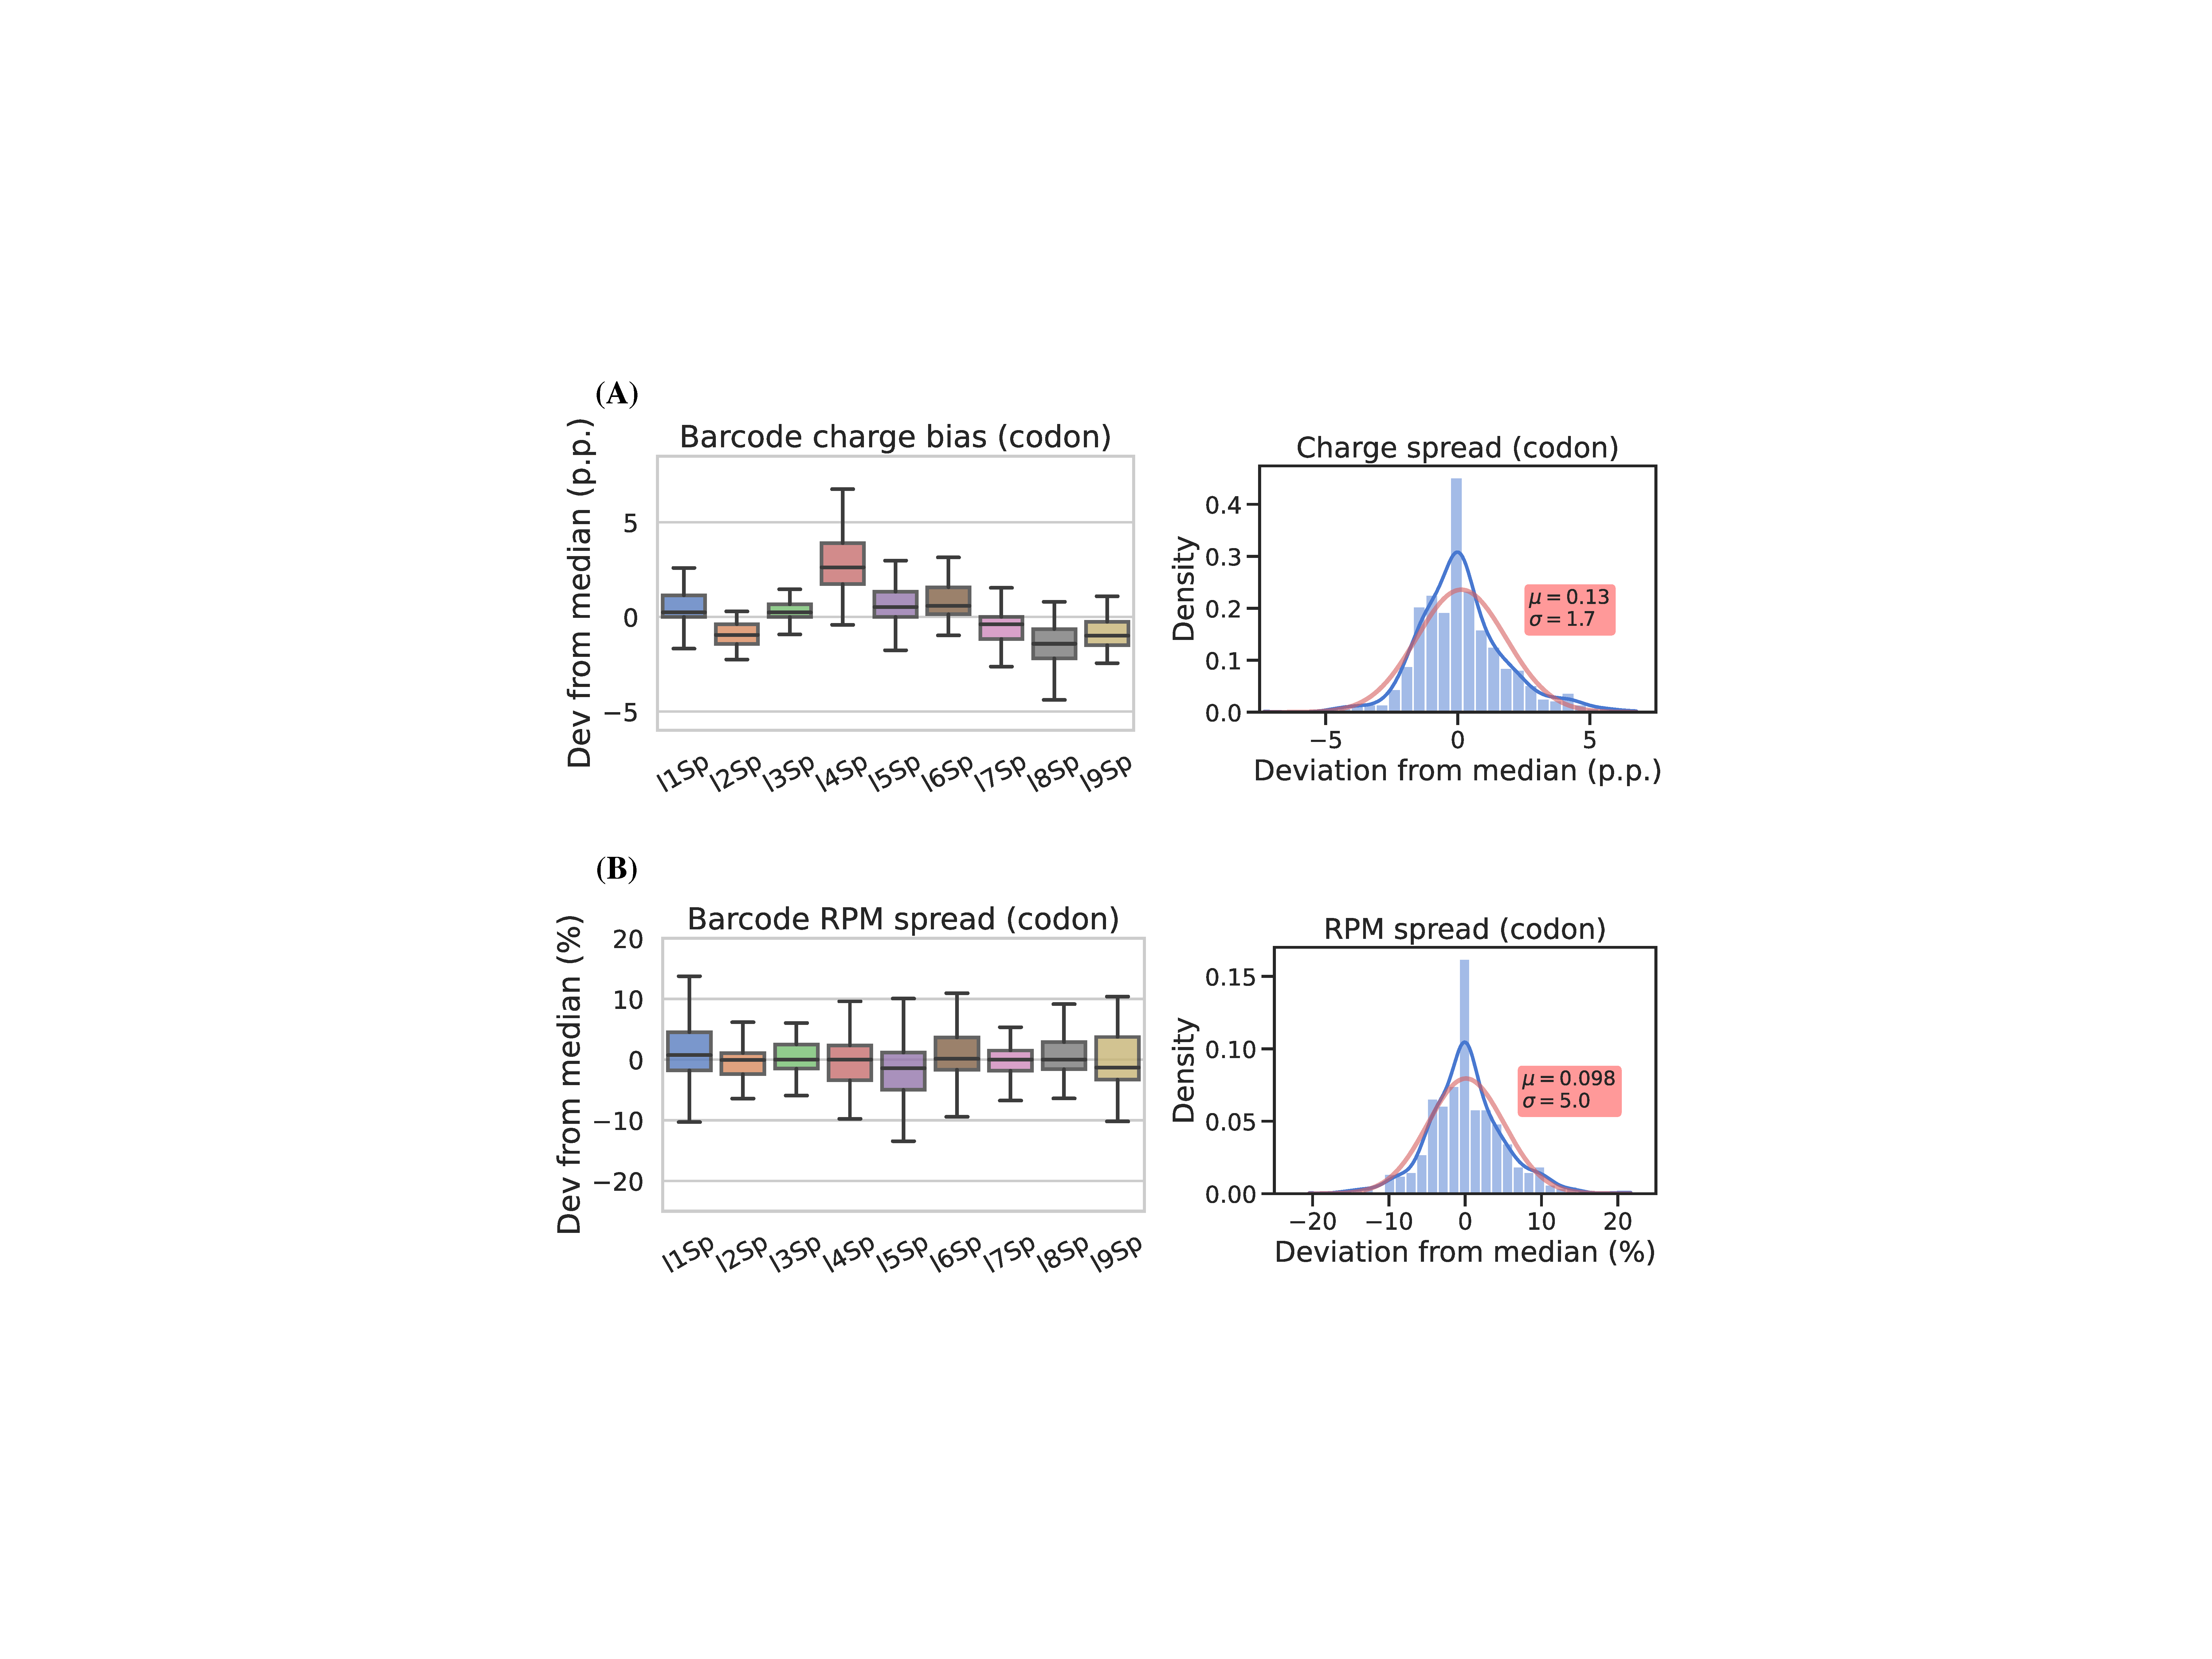
\includegraphics[width=0.65\linewidth]{figures/Fig4.pdf}}
\caption{
Barcode replicates show high precision and no barcode bias.
Each of the nine adapters were ligated to the same sample containing a heterogeneous mix of CC and CCA-ending tRNAs.
Ligations were then pooled and submitted to the remainder of the charge tRNA-Seq protocol.
\textbf{(A)} The percentage point deviation from the median charge at the codon level, grouped by barcode identity (left) or shown summarized as a density plot (right).
\textbf{(B)} The percentage deviation from the median RPM at the codon level, grouped by barcode identity (left) or shown summarized as a density plot (right).
Density plots are provided with kernel density estimate (KDE) in blue, normal distribution estimate in red and inserts with mean ($\mu$) and standard deviation ($\sigma$).
For plots of transcript level data see \FIGSUPP[Fig4]{f4S1}.
}
\label{fig:Fig4}

\figsupp[Charge and RPM deviation at the transcript level.]{
Similar to \FIG{Fig4}, but at the transcript level.
}{\fbox{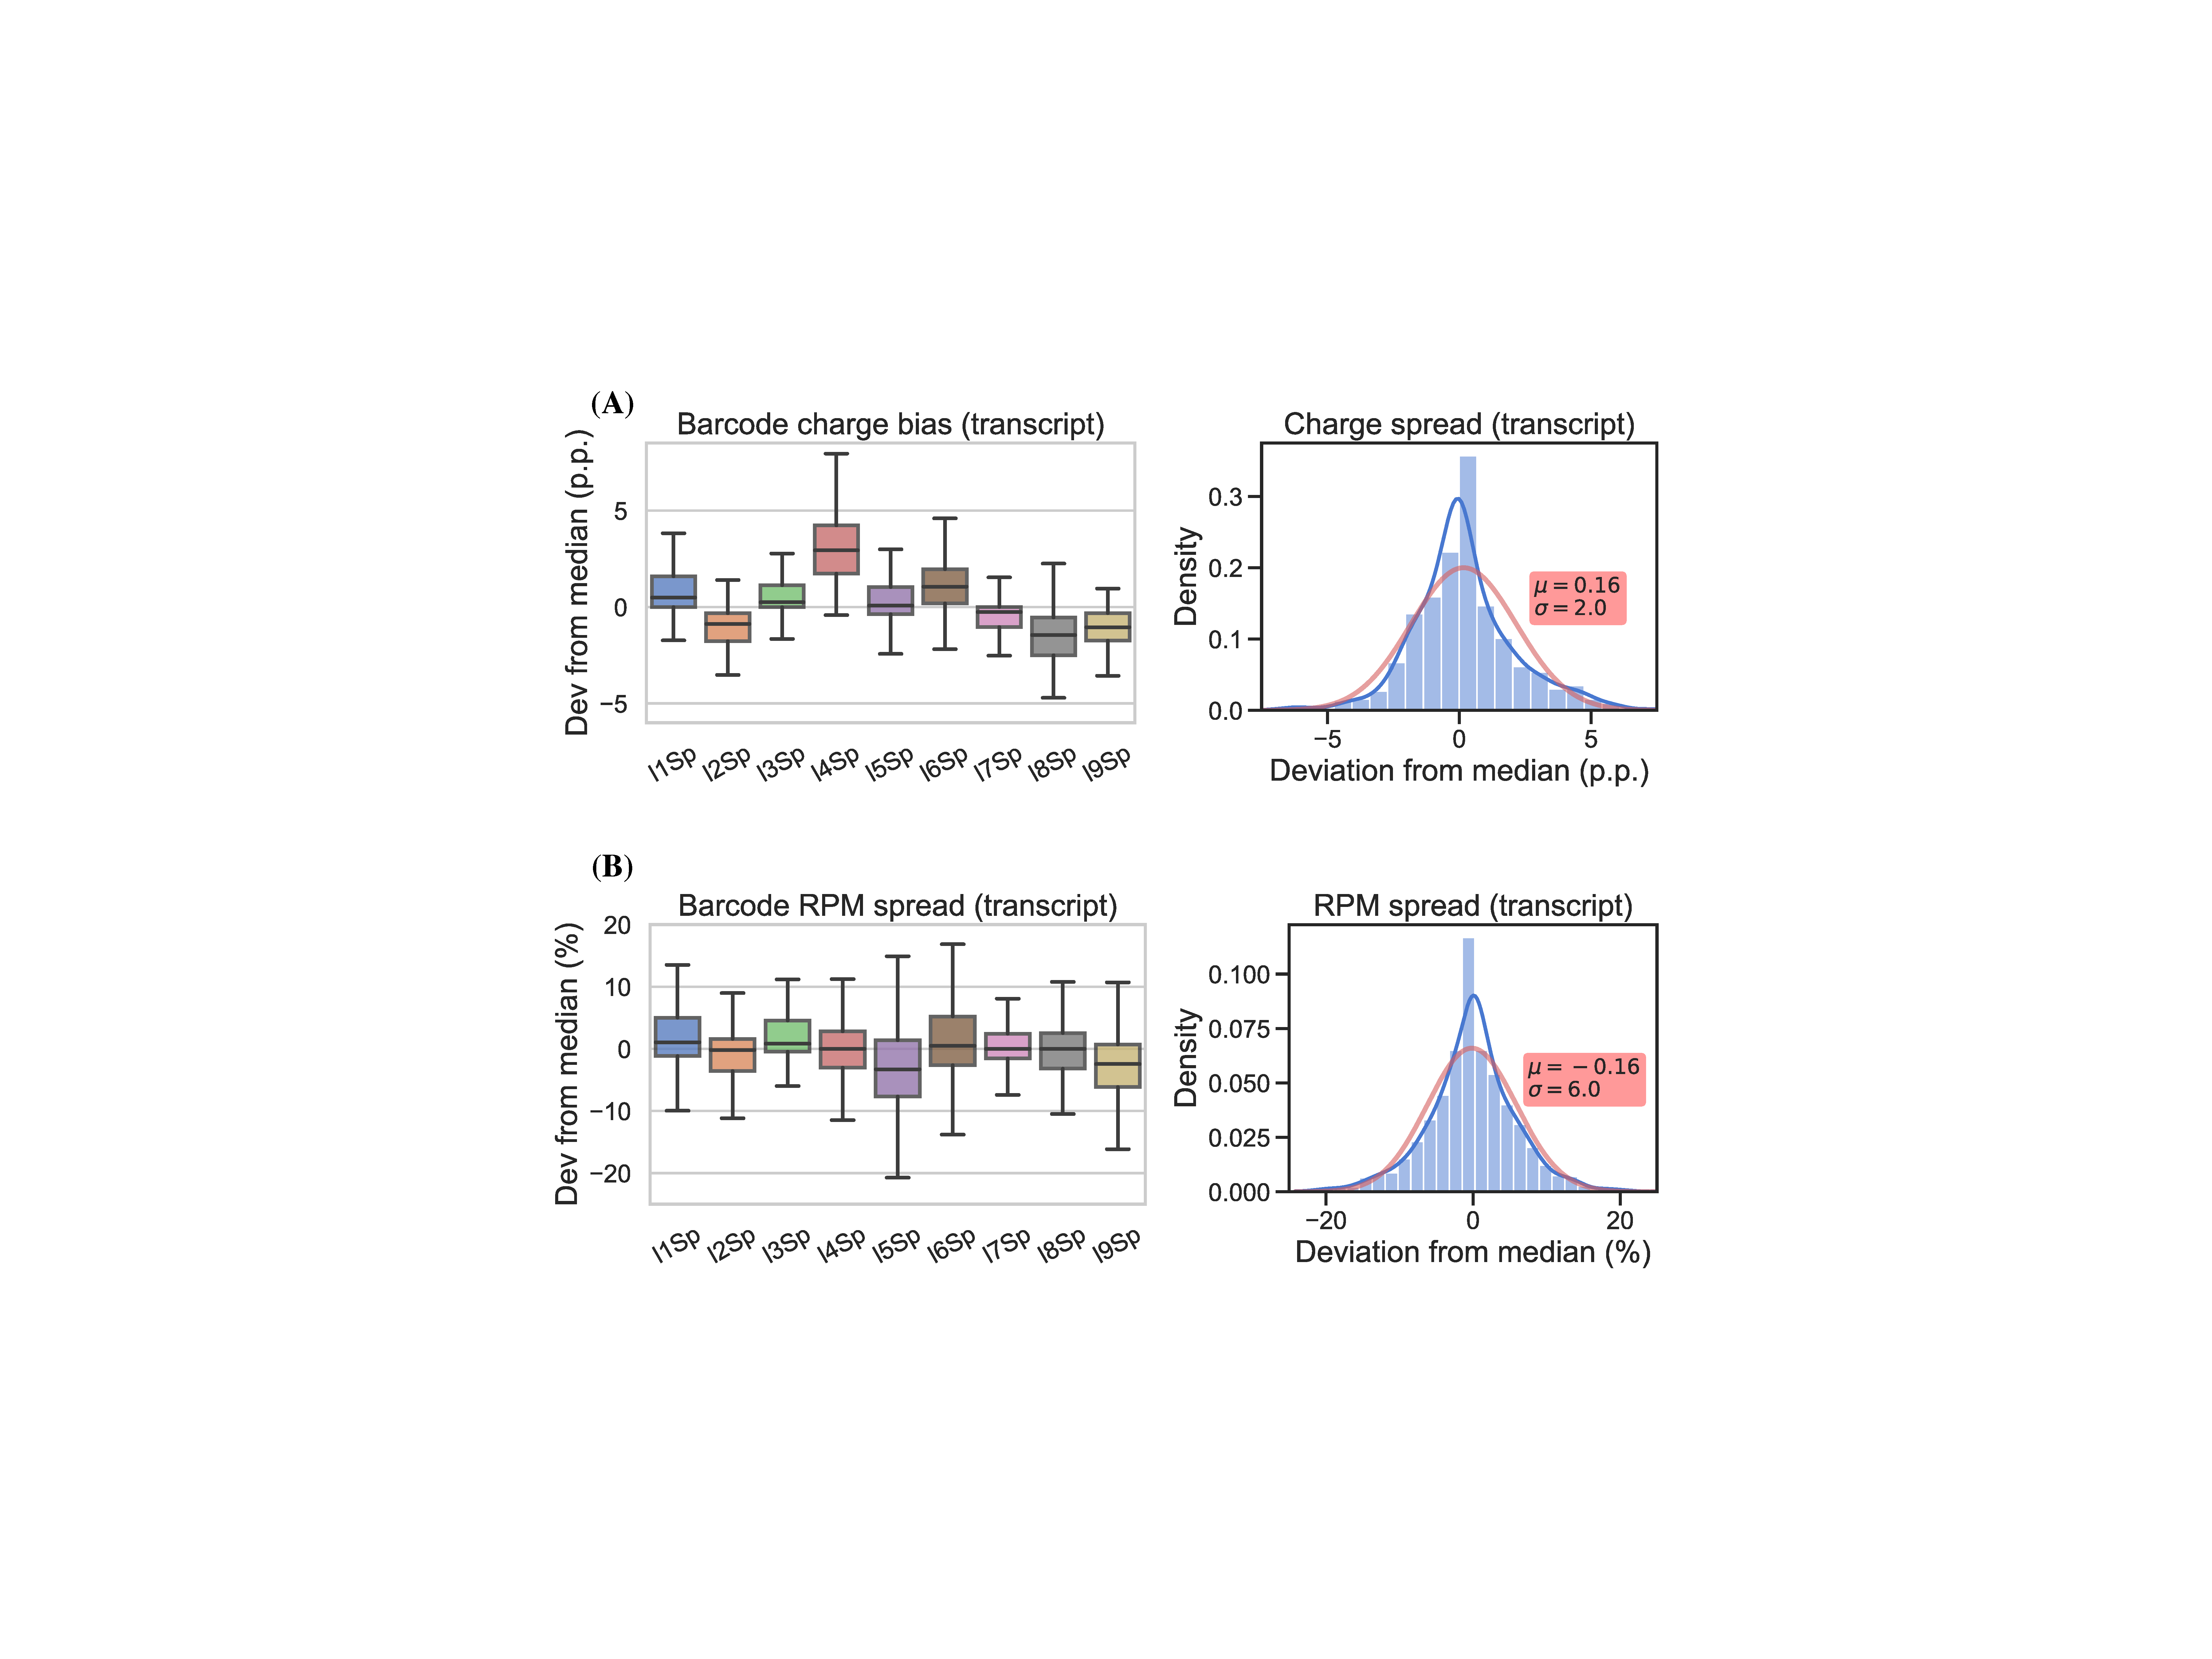
\includegraphics[width=0.65\linewidth]{figures/Fig4S1.pdf}}}\label{figsupp:f4S1}

\figsupp[Best and worst barcode replicates.]{
Best and worst pairwise comparisons between barcode replicates.
Sorting pairwise comparisons between barcode replicates according to the sum of squared differences and showing the best and worst either at the transcript or codon level.
\textbf{(A)} For charge levels, adapter l4Sp tends to overestimate charge.
\textbf{(B)} For RPM levels.
For all plots the red line is proportionality.
}{\fbox{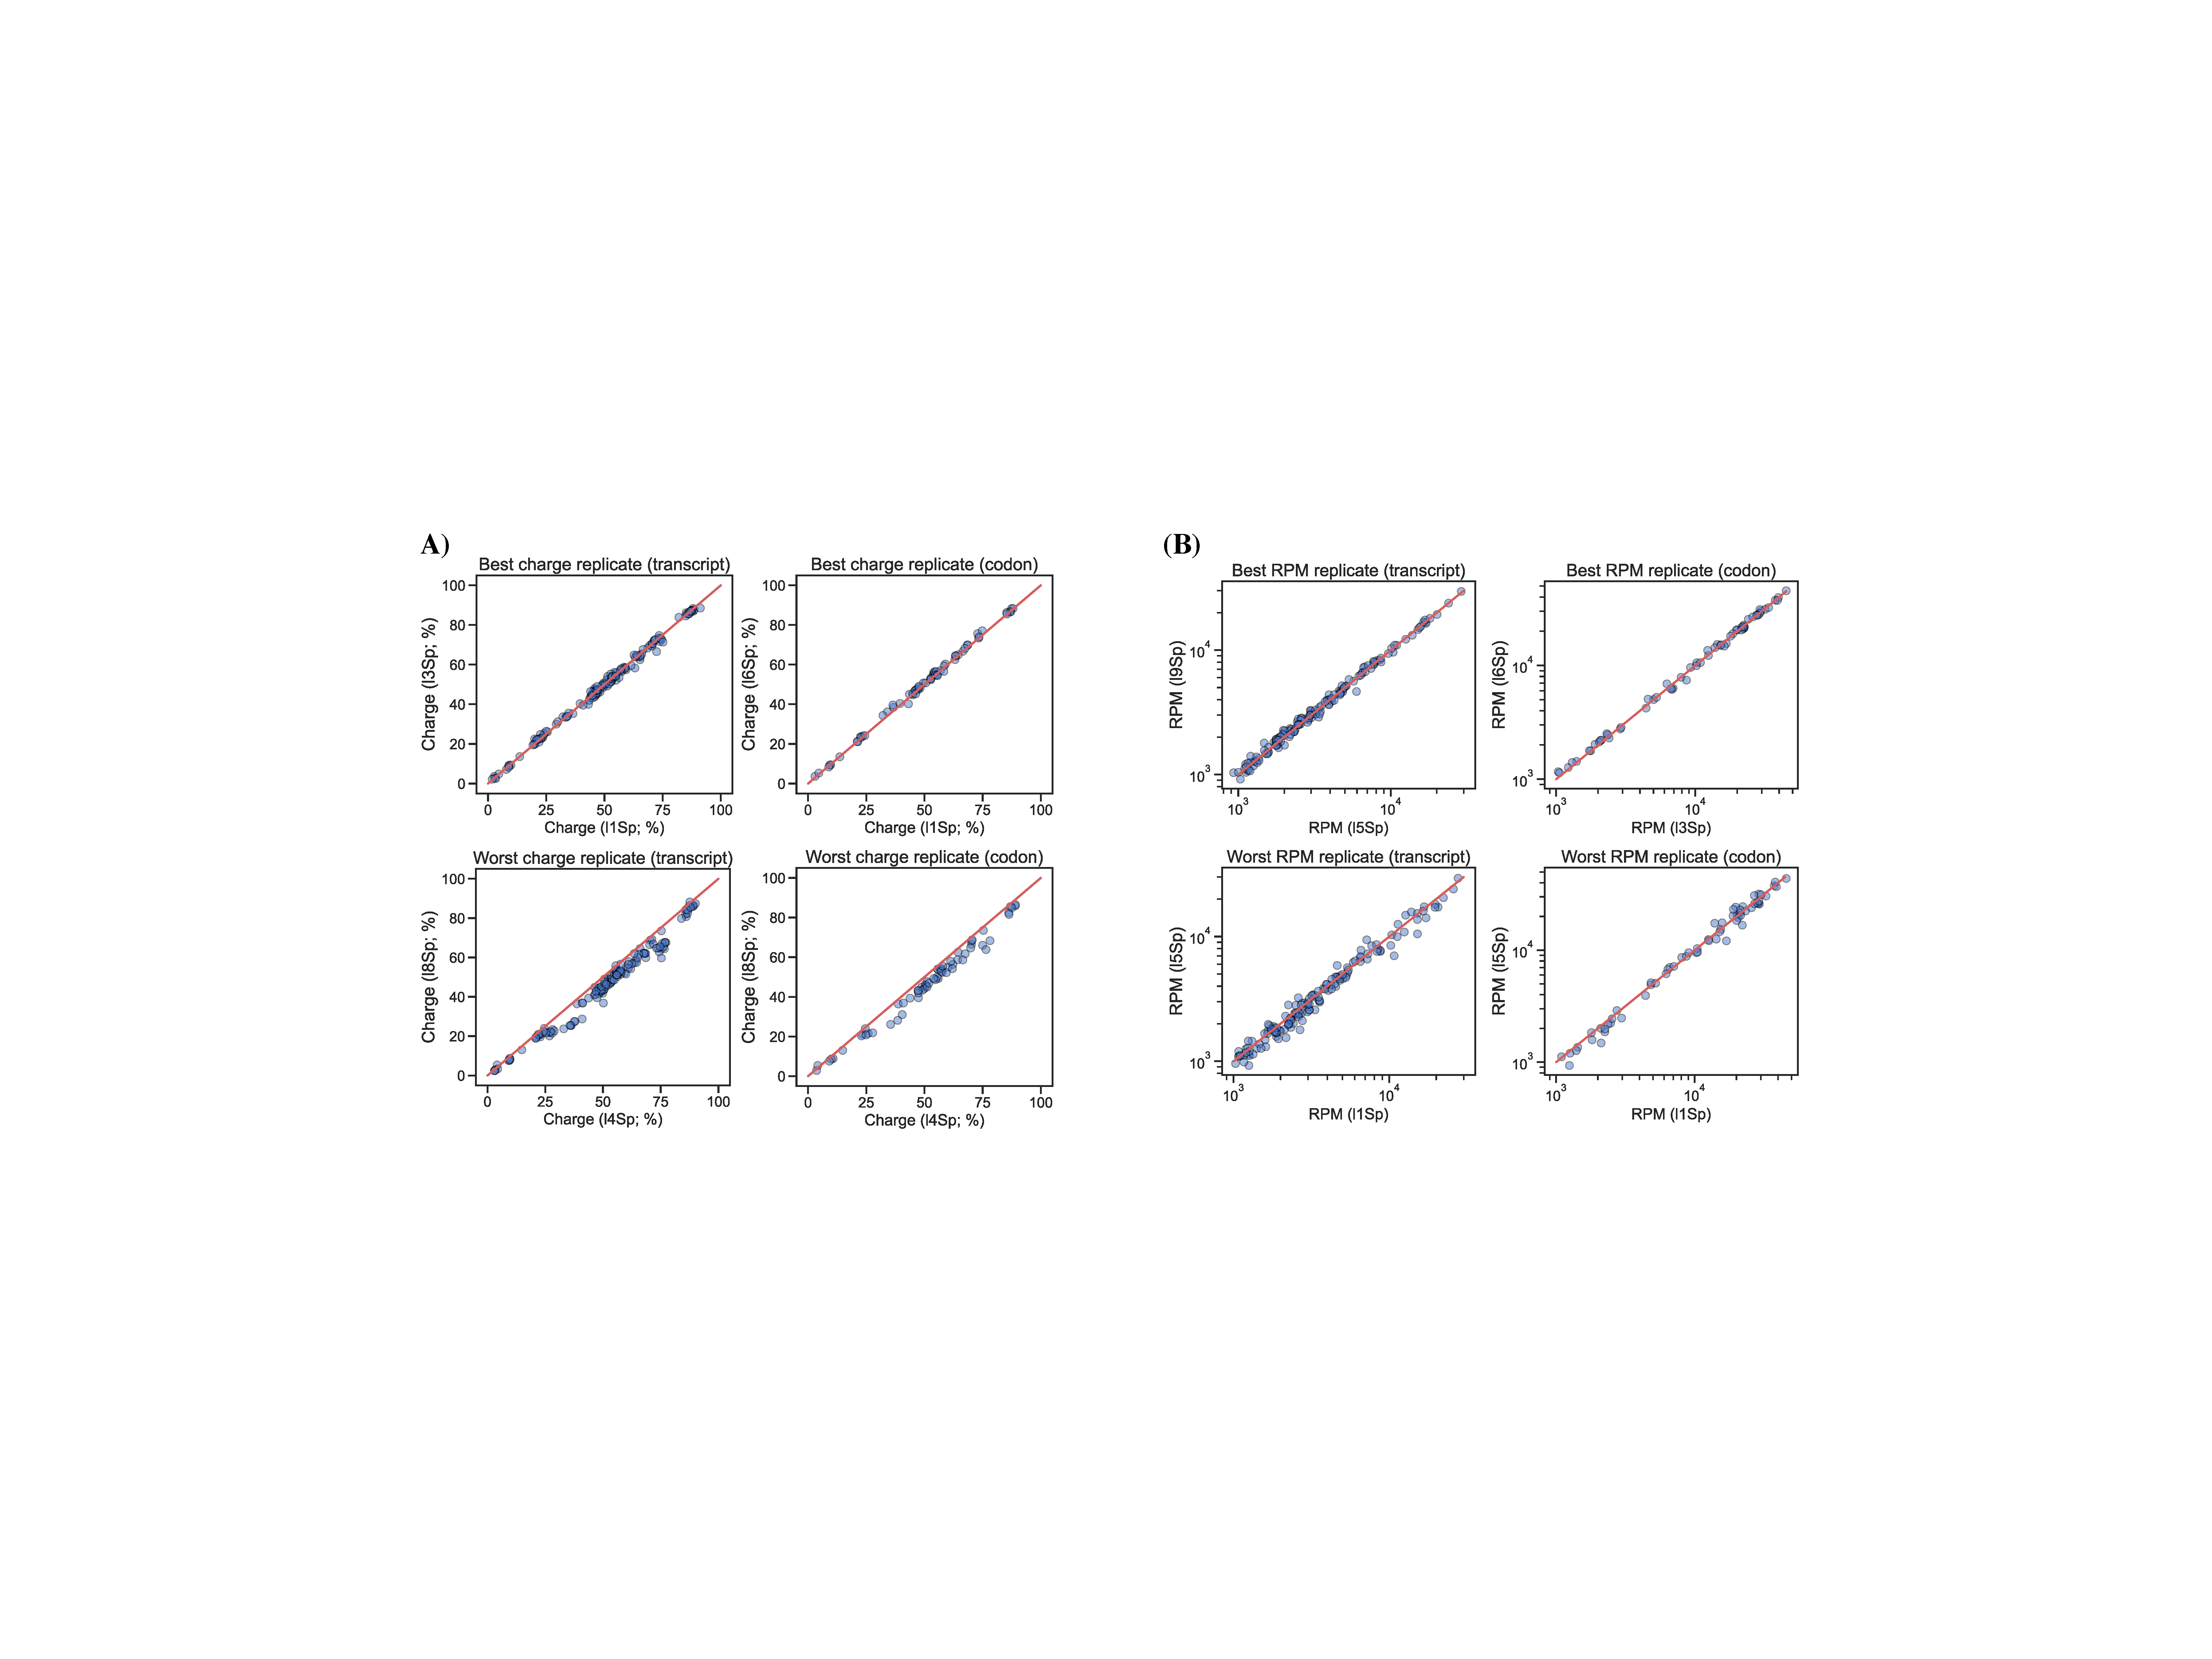
\includegraphics[width=.98\linewidth]{figures/Fig4S2.pdf}}}\label{figsupp:f4S2}
\end{figure}






\subsection{Charge titration shows high accuracy}
Testing the accuracy of charge measurements is a much harder problem.
Spiking in a defined ratio of CC and CCA-ending oligo to the ligation reaction is a common approach, but it ignores the possible effect of the Whitfeld reaction.
It is also possible to compare to charge measured by Northern blotting, but this presents a different set of issues with probe annealing, band resolution etc.
As an alternative, we made a charge titration by mixing different proportions of intact and deacylated RNA allowing us to predict and measure charge levels of over 150 transcripts (\FIG{Fig5}, panel A).
The results showed excellent proportionality between predicted and measured charge across the full range of values (\FIG{Fig5}, panel B), thus indicating that the charge measurements are highly accurate.
This experiment also confirmed our previous observations that barcode bias is limited to the l4Sp adapter which is overestimating charge (\FIG{Fig5}, panel C).
Additionally, no bias was found in independently prepared sequencing libraries or any of the different mixing proportions of intact and deacylated RNA (\FIGSUPP[Fig5]{f5S2}).

Inspired by \cite{Evans2017-st}, which used radiolabeling techniques to generate a single accurate tRNA charge reference point, we developed a 50\% charge control using 3′ phosphorylation as protection from periodate oxidation.
This control was spiked into samples before the Whitfeld reaction and showed a mean charge of 50.36\% and a standard deviation of 1.11 percentage points (\FIGSUPP[Fig5]{f5S3}, panel B), thus further validating the measurement accuracy of our method.

\begin{figure}[ht!]
\centering
\fbox{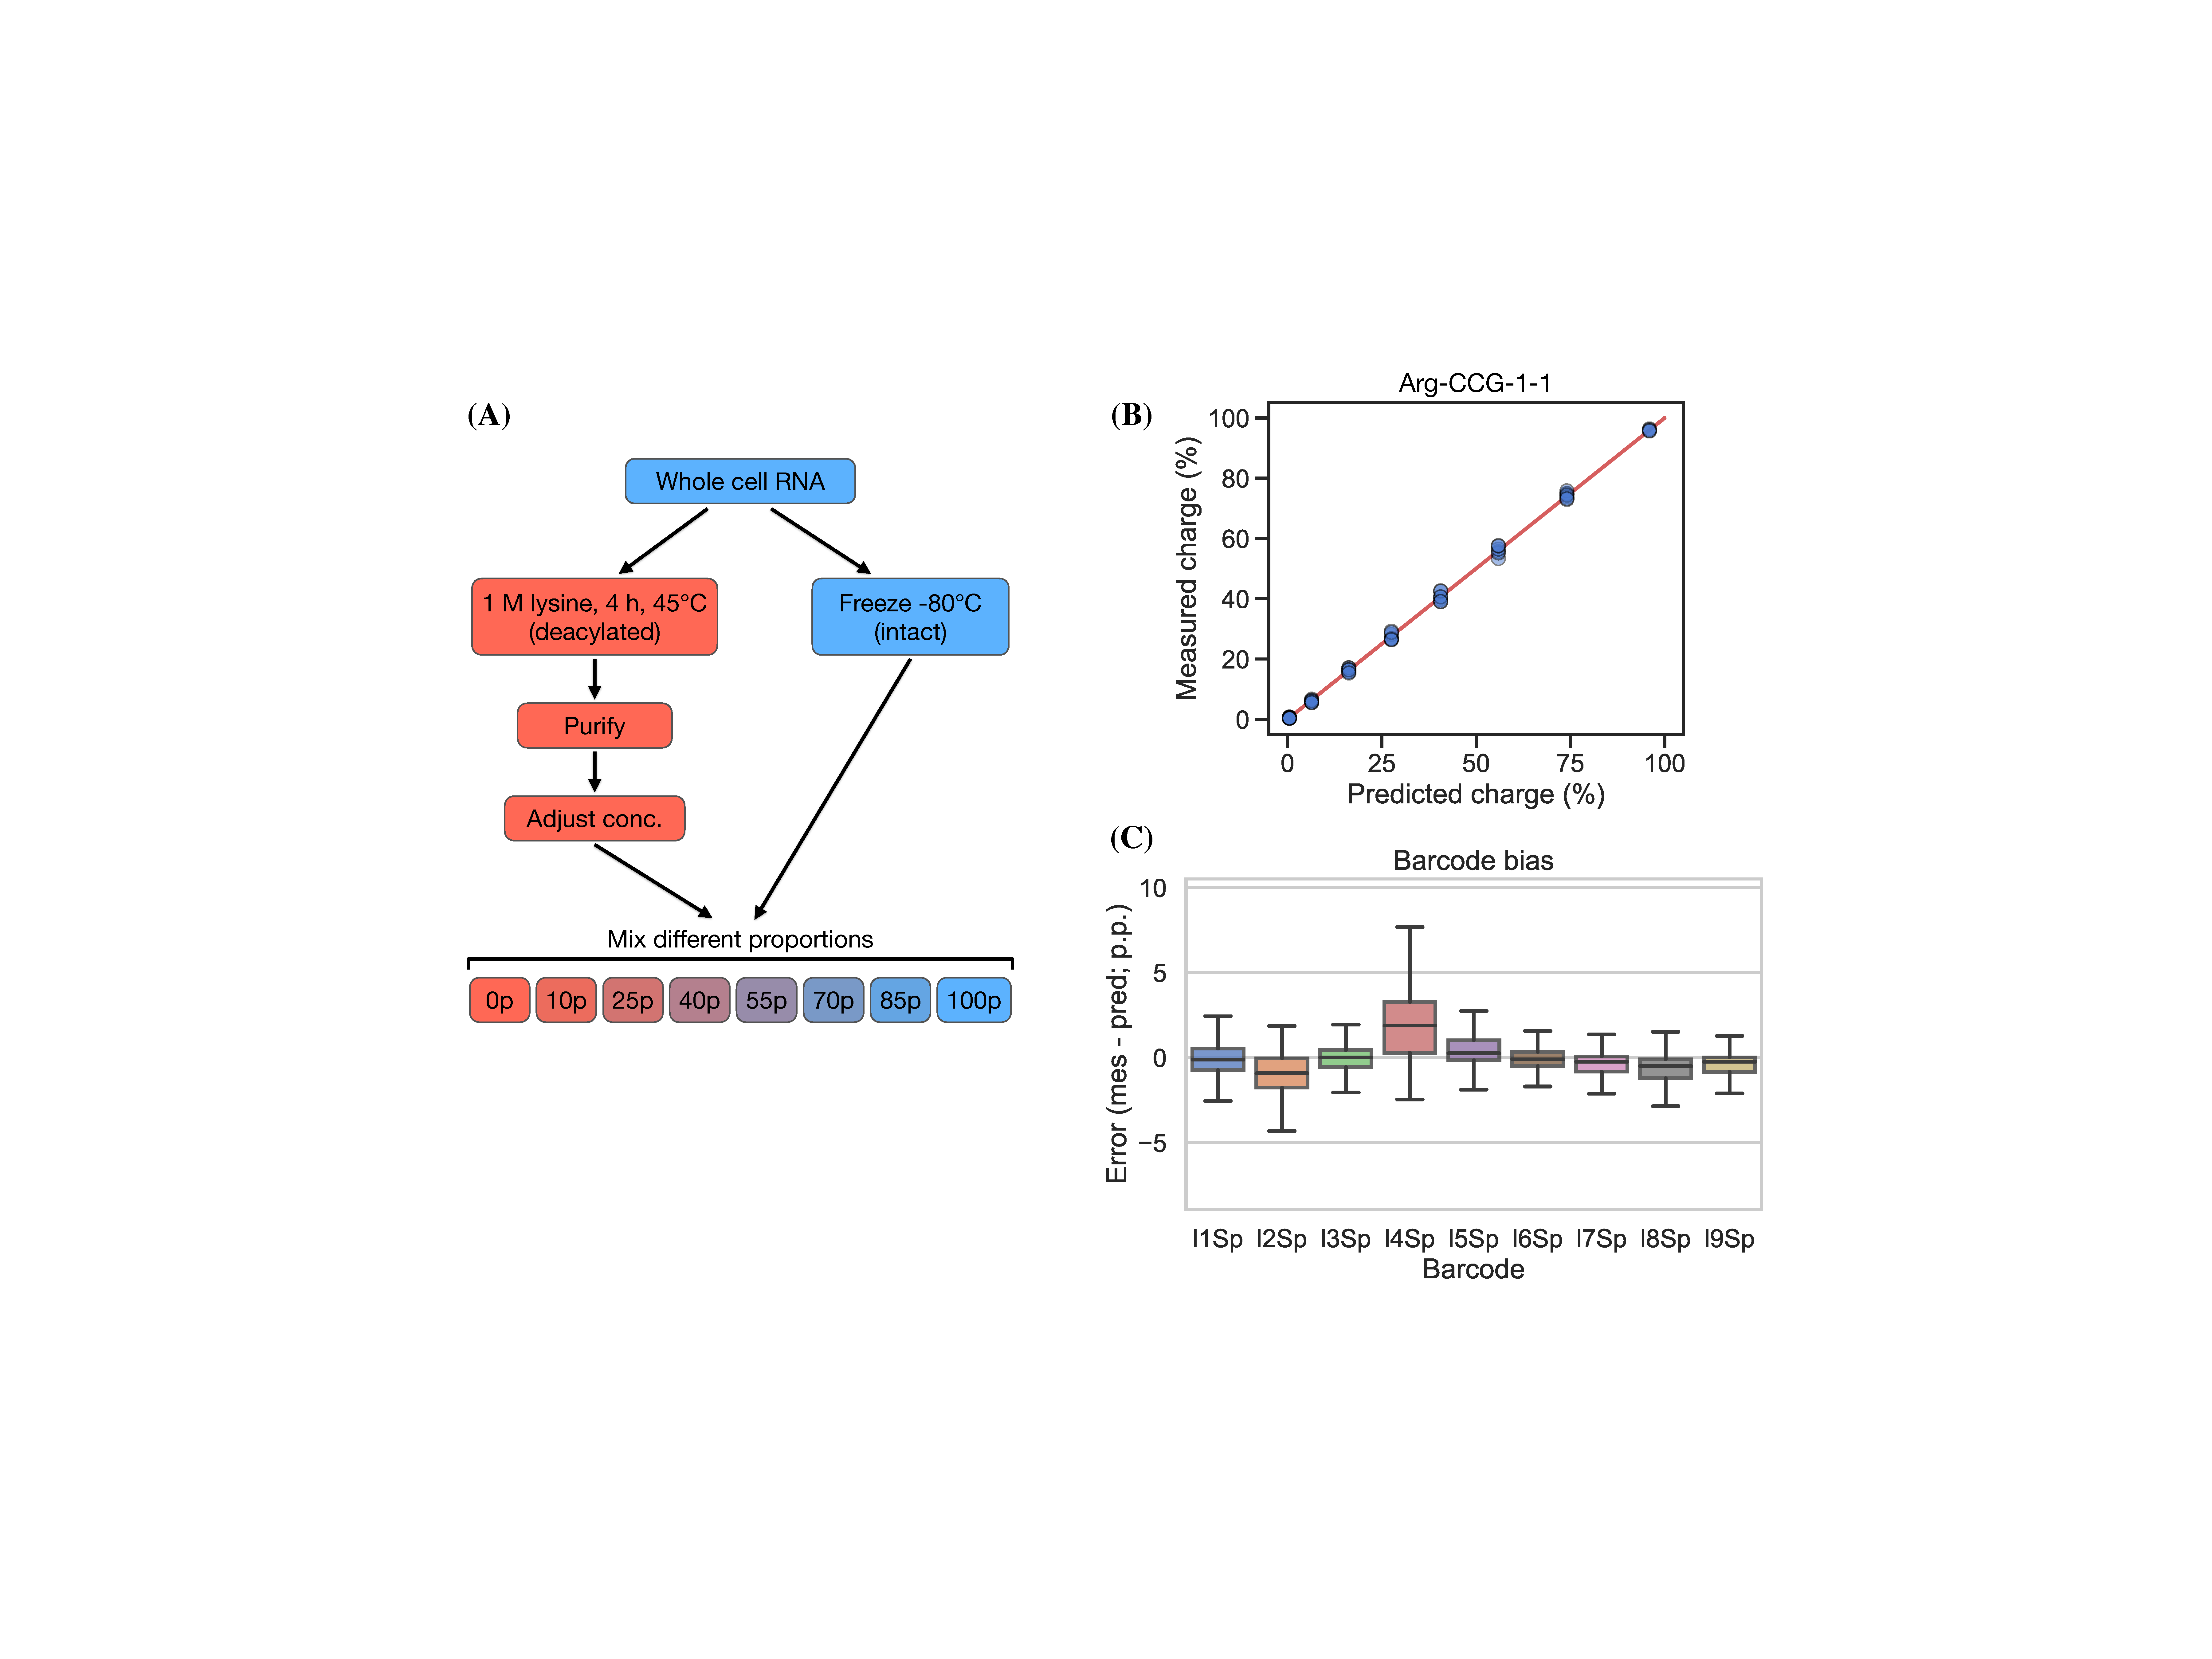
\includegraphics[width=0.65\linewidth]{figures/Fig5.pdf}}
\caption{
Charge titration shows linearity over the full range of charge measurements.
\textbf{(A)} Schematic illustration of the method to generate samples with predictable charge percentages.
\textbf{(B)} Titration data for a representative tRNA transcript, Leu-AAG-2-1, with the red line indicating proportionality between predicted and measured charge.
For reference, the best and worst fitting tRNA transcripts are shown in \FIGSUPP[Fig5]{f5S1}.
\textbf{(C)} Error binned by adapter barcode.
Error is the percentage point difference between the measured vs. predicted charge for all transcripts in the bin.
}
\label{fig:Fig5}

\figsupp[Best and worst fitting transcripts for charge titration.]{
The best and worst transcript when ranked based on the sum of squared differences between the measured and predicted charge.
Related to the representative (i.e. ranked as the median) transcript shown in \FIG{Fig5}, panel B.
}{\fbox{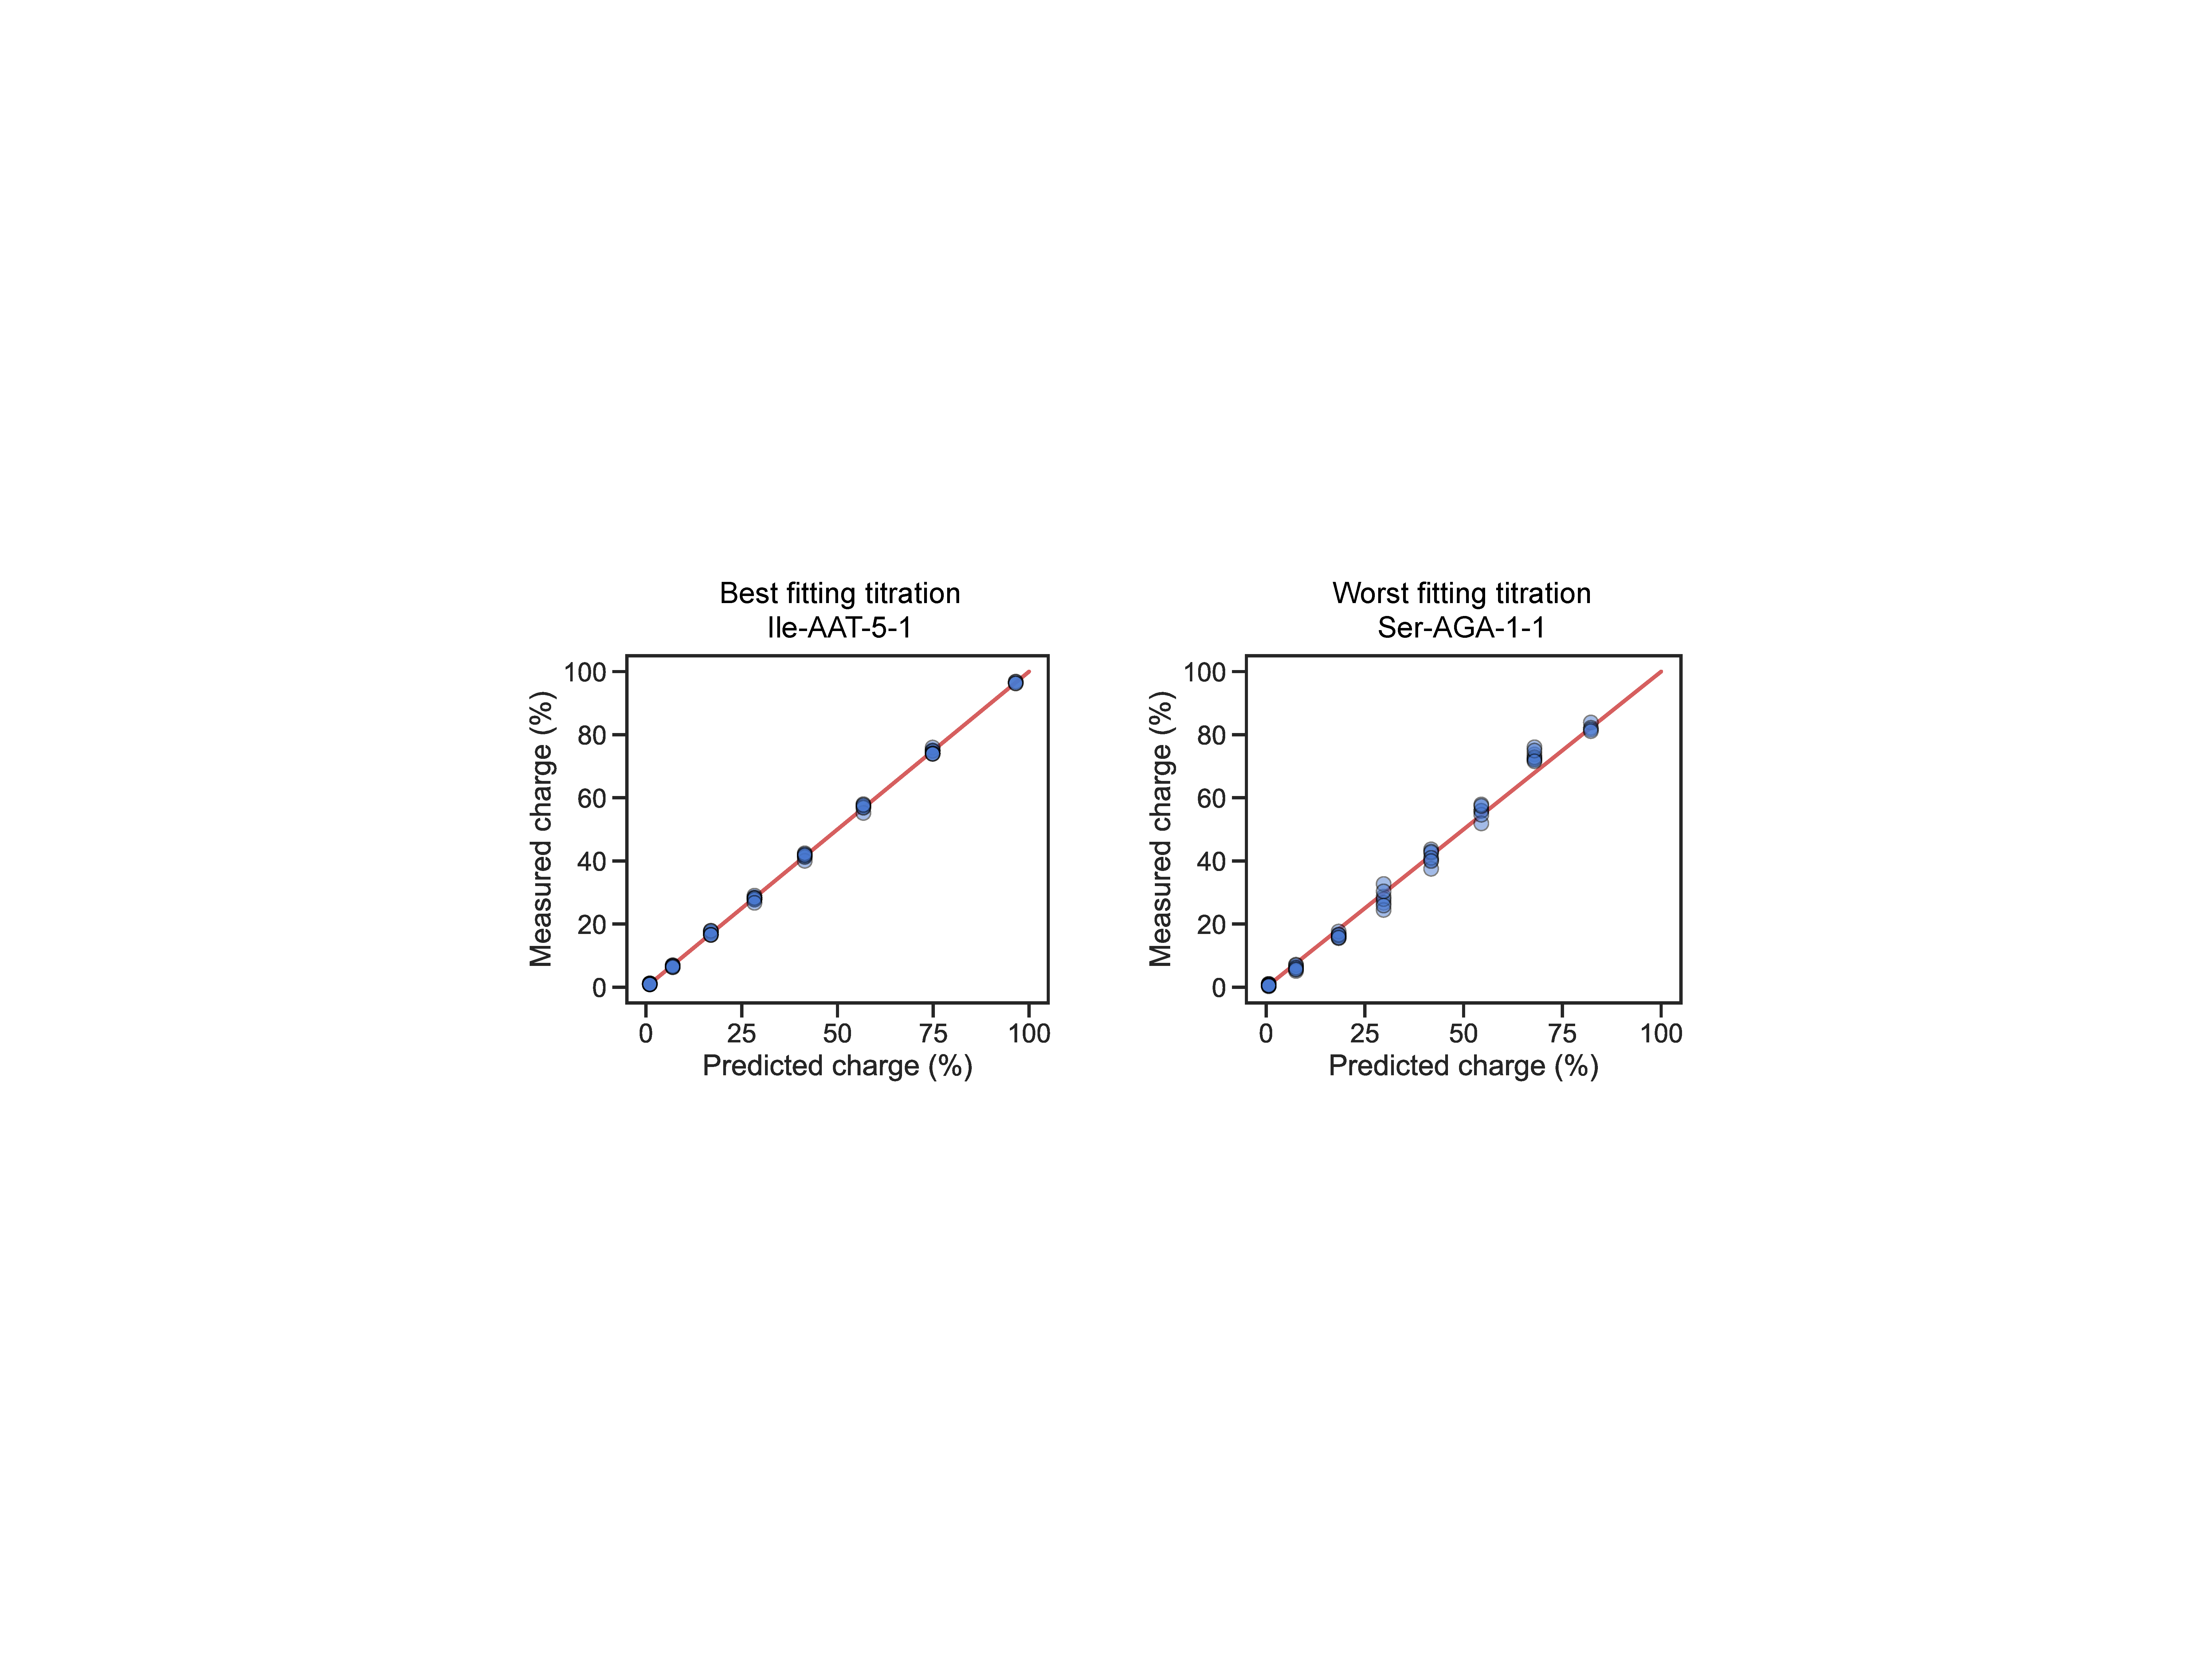
\includegraphics[width=0.7\linewidth]{figures/Fig5S1.pdf}}}\label{figsupp:f5S1}

\figsupp[Error binned by sequencing run and titration sample.]{
Charge titration prediction error binned by sequencing run and titration sample.
\textbf{(A)} Run-to-run bias of two independently prepared sequencing libraries, sequenced on different days.
\textbf{(B)} Error distribution binned by titration sample.
In both panels, error is the percentage point difference between the measured vs. predicted charge for all transcripts in the bin.
}{\fbox{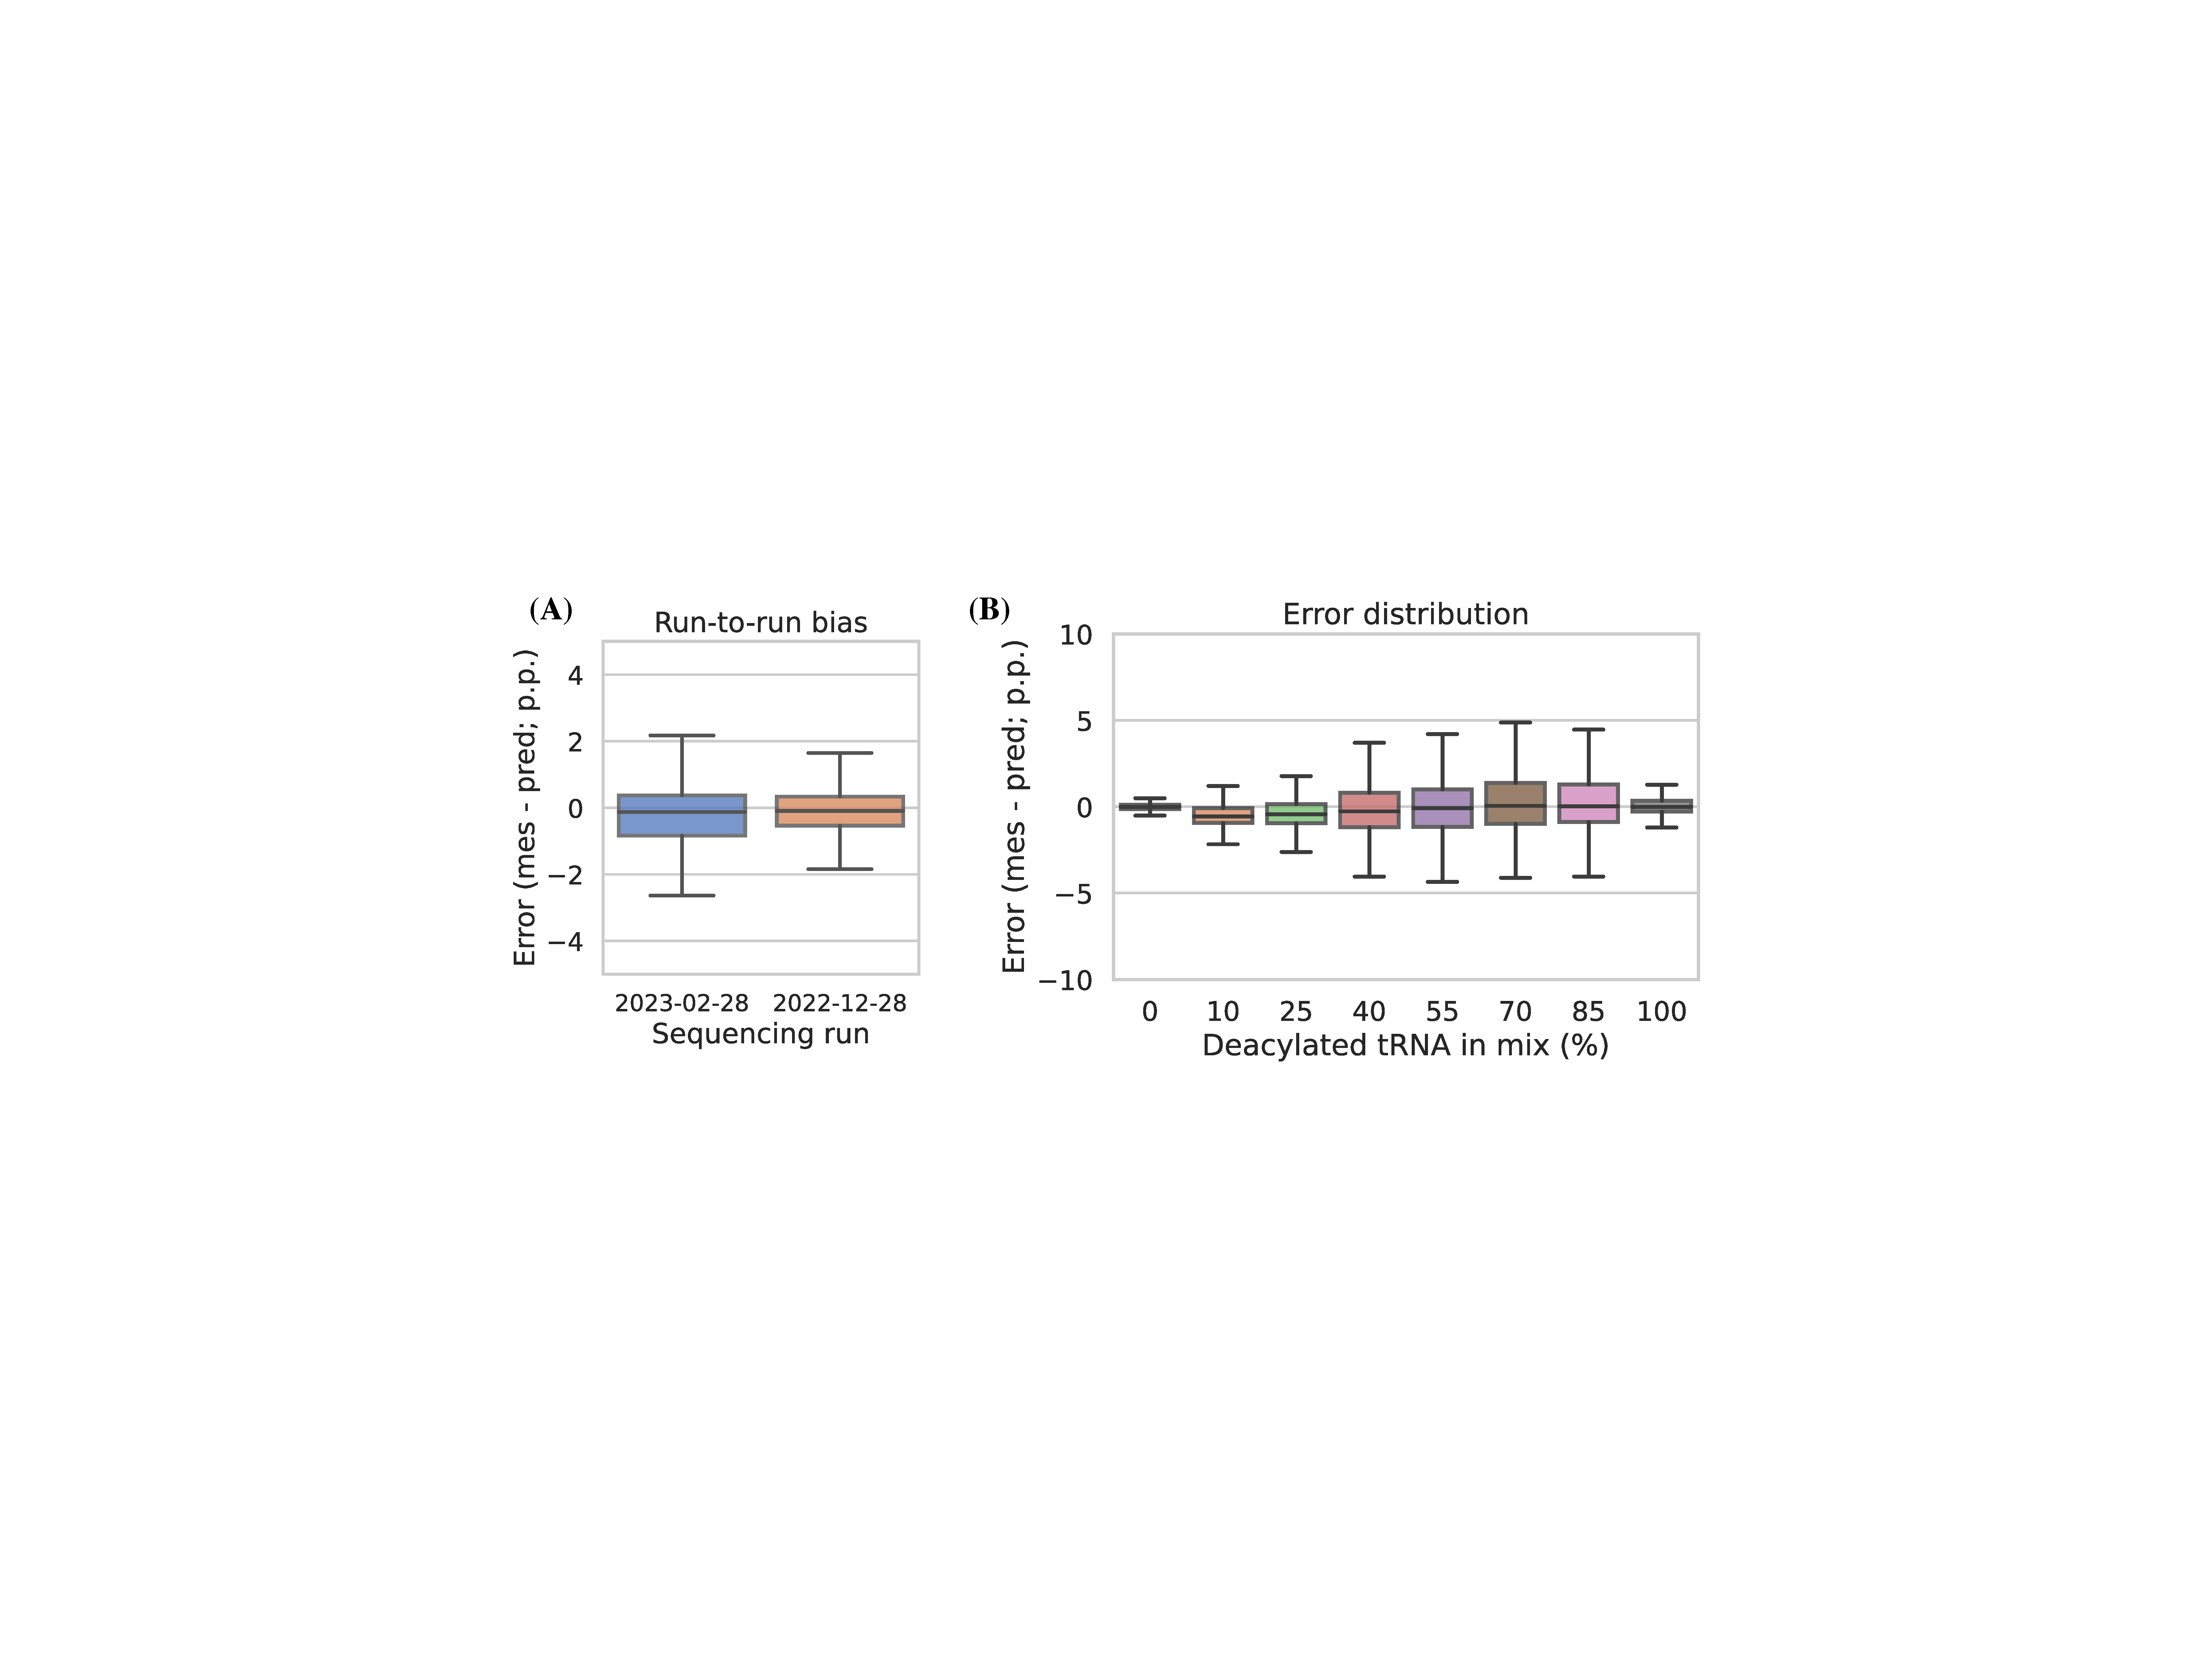
\includegraphics[width=0.65\linewidth]{figures/Fig5S2.pdf}}}\label{figsupp:f5S2}

\figsupp[Spike-in control for 50\% charge.]{
Spike-in control for 50\% charge using the E.coli tRNA-Thr-CGT oligo.
\textbf{(A)} Ligation between E.coli tRNA-Thr-CCA-Phos and l8Sp is completely blocked indicating $\sim$100\% 3′ phosphorylation.
CCA-P, E.coli tRNA-Thr-CCA-Phos.
CCA, E.coli tRNA-Thr-CCA.
50/50, equal mix of CCA-p and CCA.
\textbf{(B)} E.coli tRNA-Thr spike-in charge measured for samples prepared with an equimolar mix of E.coli tRNA-Thr-CCA-Phos and E.coli tRNA-Thr-CCA.
The red dashed line indicates 50\% charge.
}{\fbox{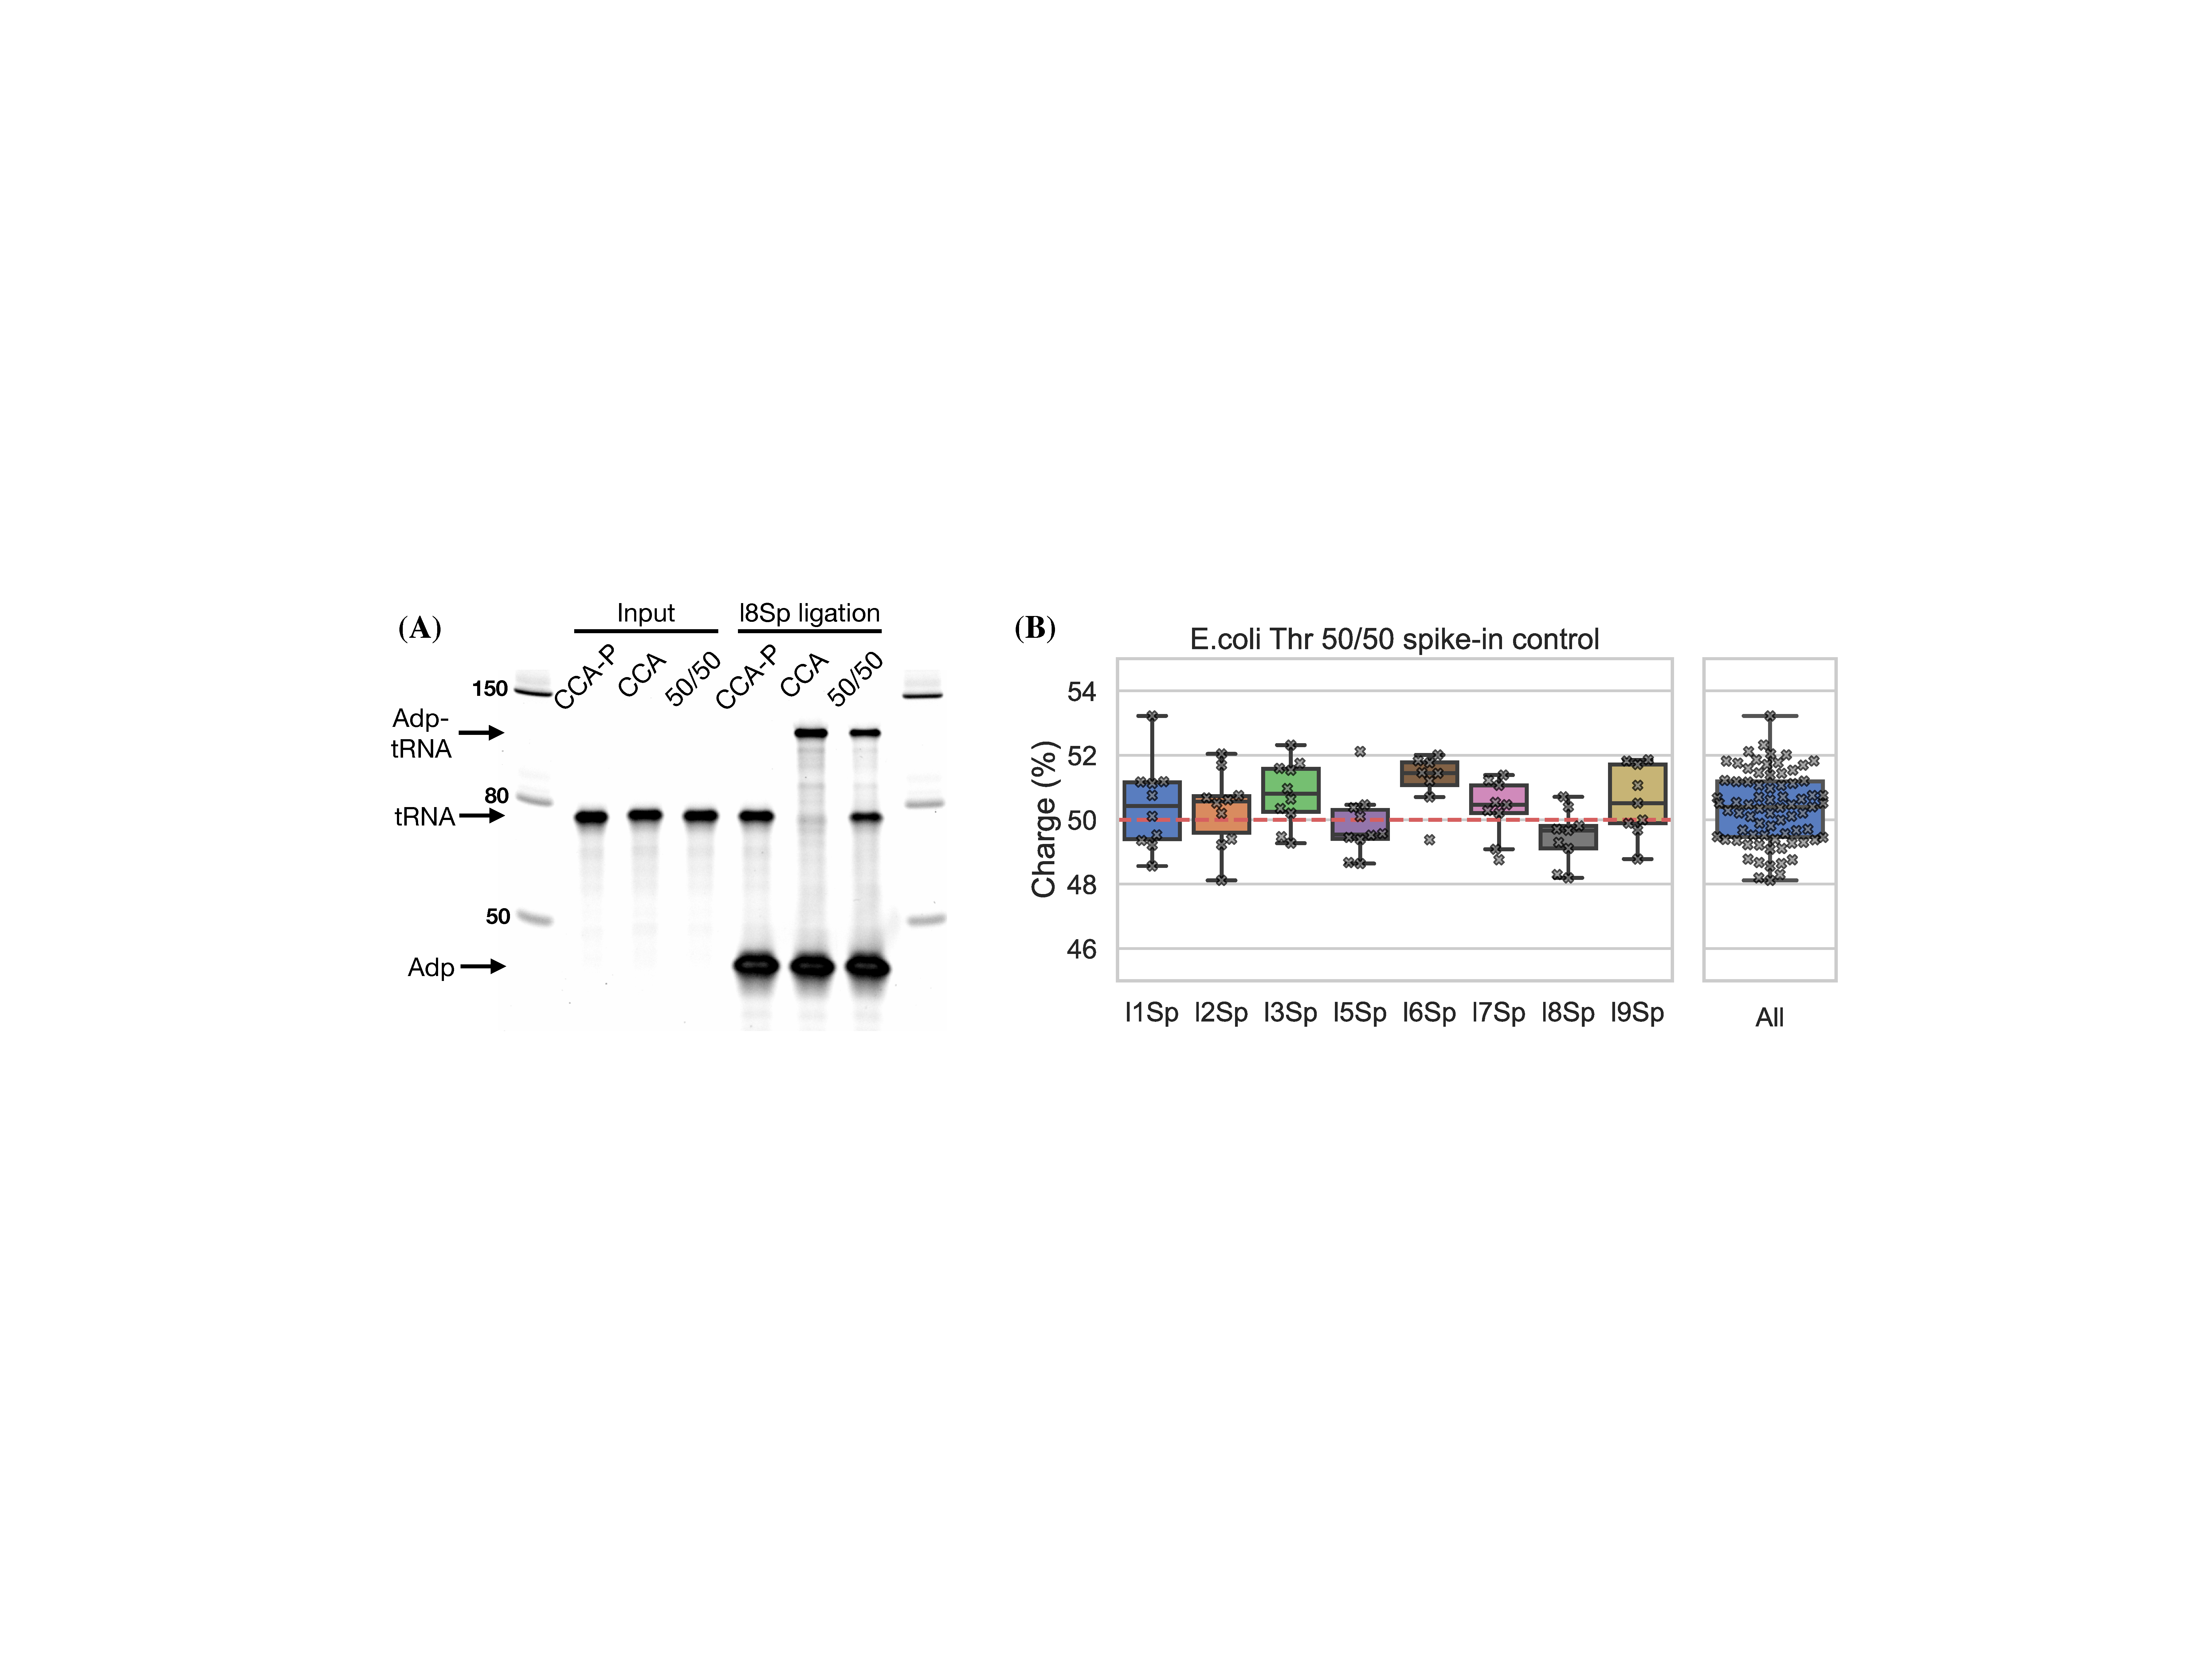
\includegraphics[width=0.85\linewidth]{figures/Fig5S3.pdf}}}\label{figsupp:f5S3}
\end{figure}





\subsection{Charge tRNA-Seq enables measurement of aminoacylation half-lifes of native tRNAs}
tRNA aminoacylations are prone to hydrolysis and the effect of pH and temperature on their decay rates has previously been studied \citep{Hentzen1972-yd}.
Interestingly, \cite{Peacock2014-wk} found that the aminoacylation half-life appeared to be determined solely by the identity of the amino acid attachment and not effected significantly by the tRNA sequence or RNA modifications.
However, most of the tRNAs used in this study were derived from in vitro transcription and only a limited set of RNA modifications were tested; additionally, the study did not cover all 20 native amino acids.
Having developed an accurate method for measuring tRNA charge on over a hundred samples in a single sequencing run, we wanted to use this to determine the aminoacylation half-lifes of tRNA transcripts with their native RNA modifications.

We used RNA purified from the H1299 cell line, starting at high tRNA charge (\FIG{Fig2}, panel F), and tracked the aminoacylation decay over time after switching to physiological buffer (pH=7.2) and incubation at 20°C similar to \cite{Peacock2014-wk}.
After sampling 11 timepoints with 4 replicates, charge measurements for each transcript were fitted to a first-order decay function to estimate the half-life of each transcripts (Supplementary file 4), as exemplified by the representative transcript Arg-TCG-2-1 (\FIG{Fig6}, panel A).
When transcripts were grouped by their cognate amino acid, we could confirm that the half-lifes are indeed determined mostly by aminoacylation identity and that they span a large 37 fold range (\FIG{Fig6}, panel B).
Our half-life estimates are highly correlated with those reported by \cite{Peacock2014-wk}, but surprisingly ours appear to be approximately 4 fold higher despite using the same incubation temperature and a similar buffer, with only slightly lower pH (7.2 vs. 7.5; \FIGSUPP[Fig6]{f6S1}, panel B).

It seems counterintuitive that the aminoacylation half-life should be completely unaffected by the tRNA sequence; however, as the amino acid is attached to the invariant CCA-end, the nucleotides most proximal to the ester bond are the same for all tRNAs.
The most proximal non-invariant nucleotide is the discriminator base.
Because we sample all transcripts, we are able to show that the discriminator base is indeed likely to influence the half-life and that a purine base leads to longer half-life than a uracil (\FIG{Fig6}, panel C).

\begin{figure}[ht!]
\centering
\fbox{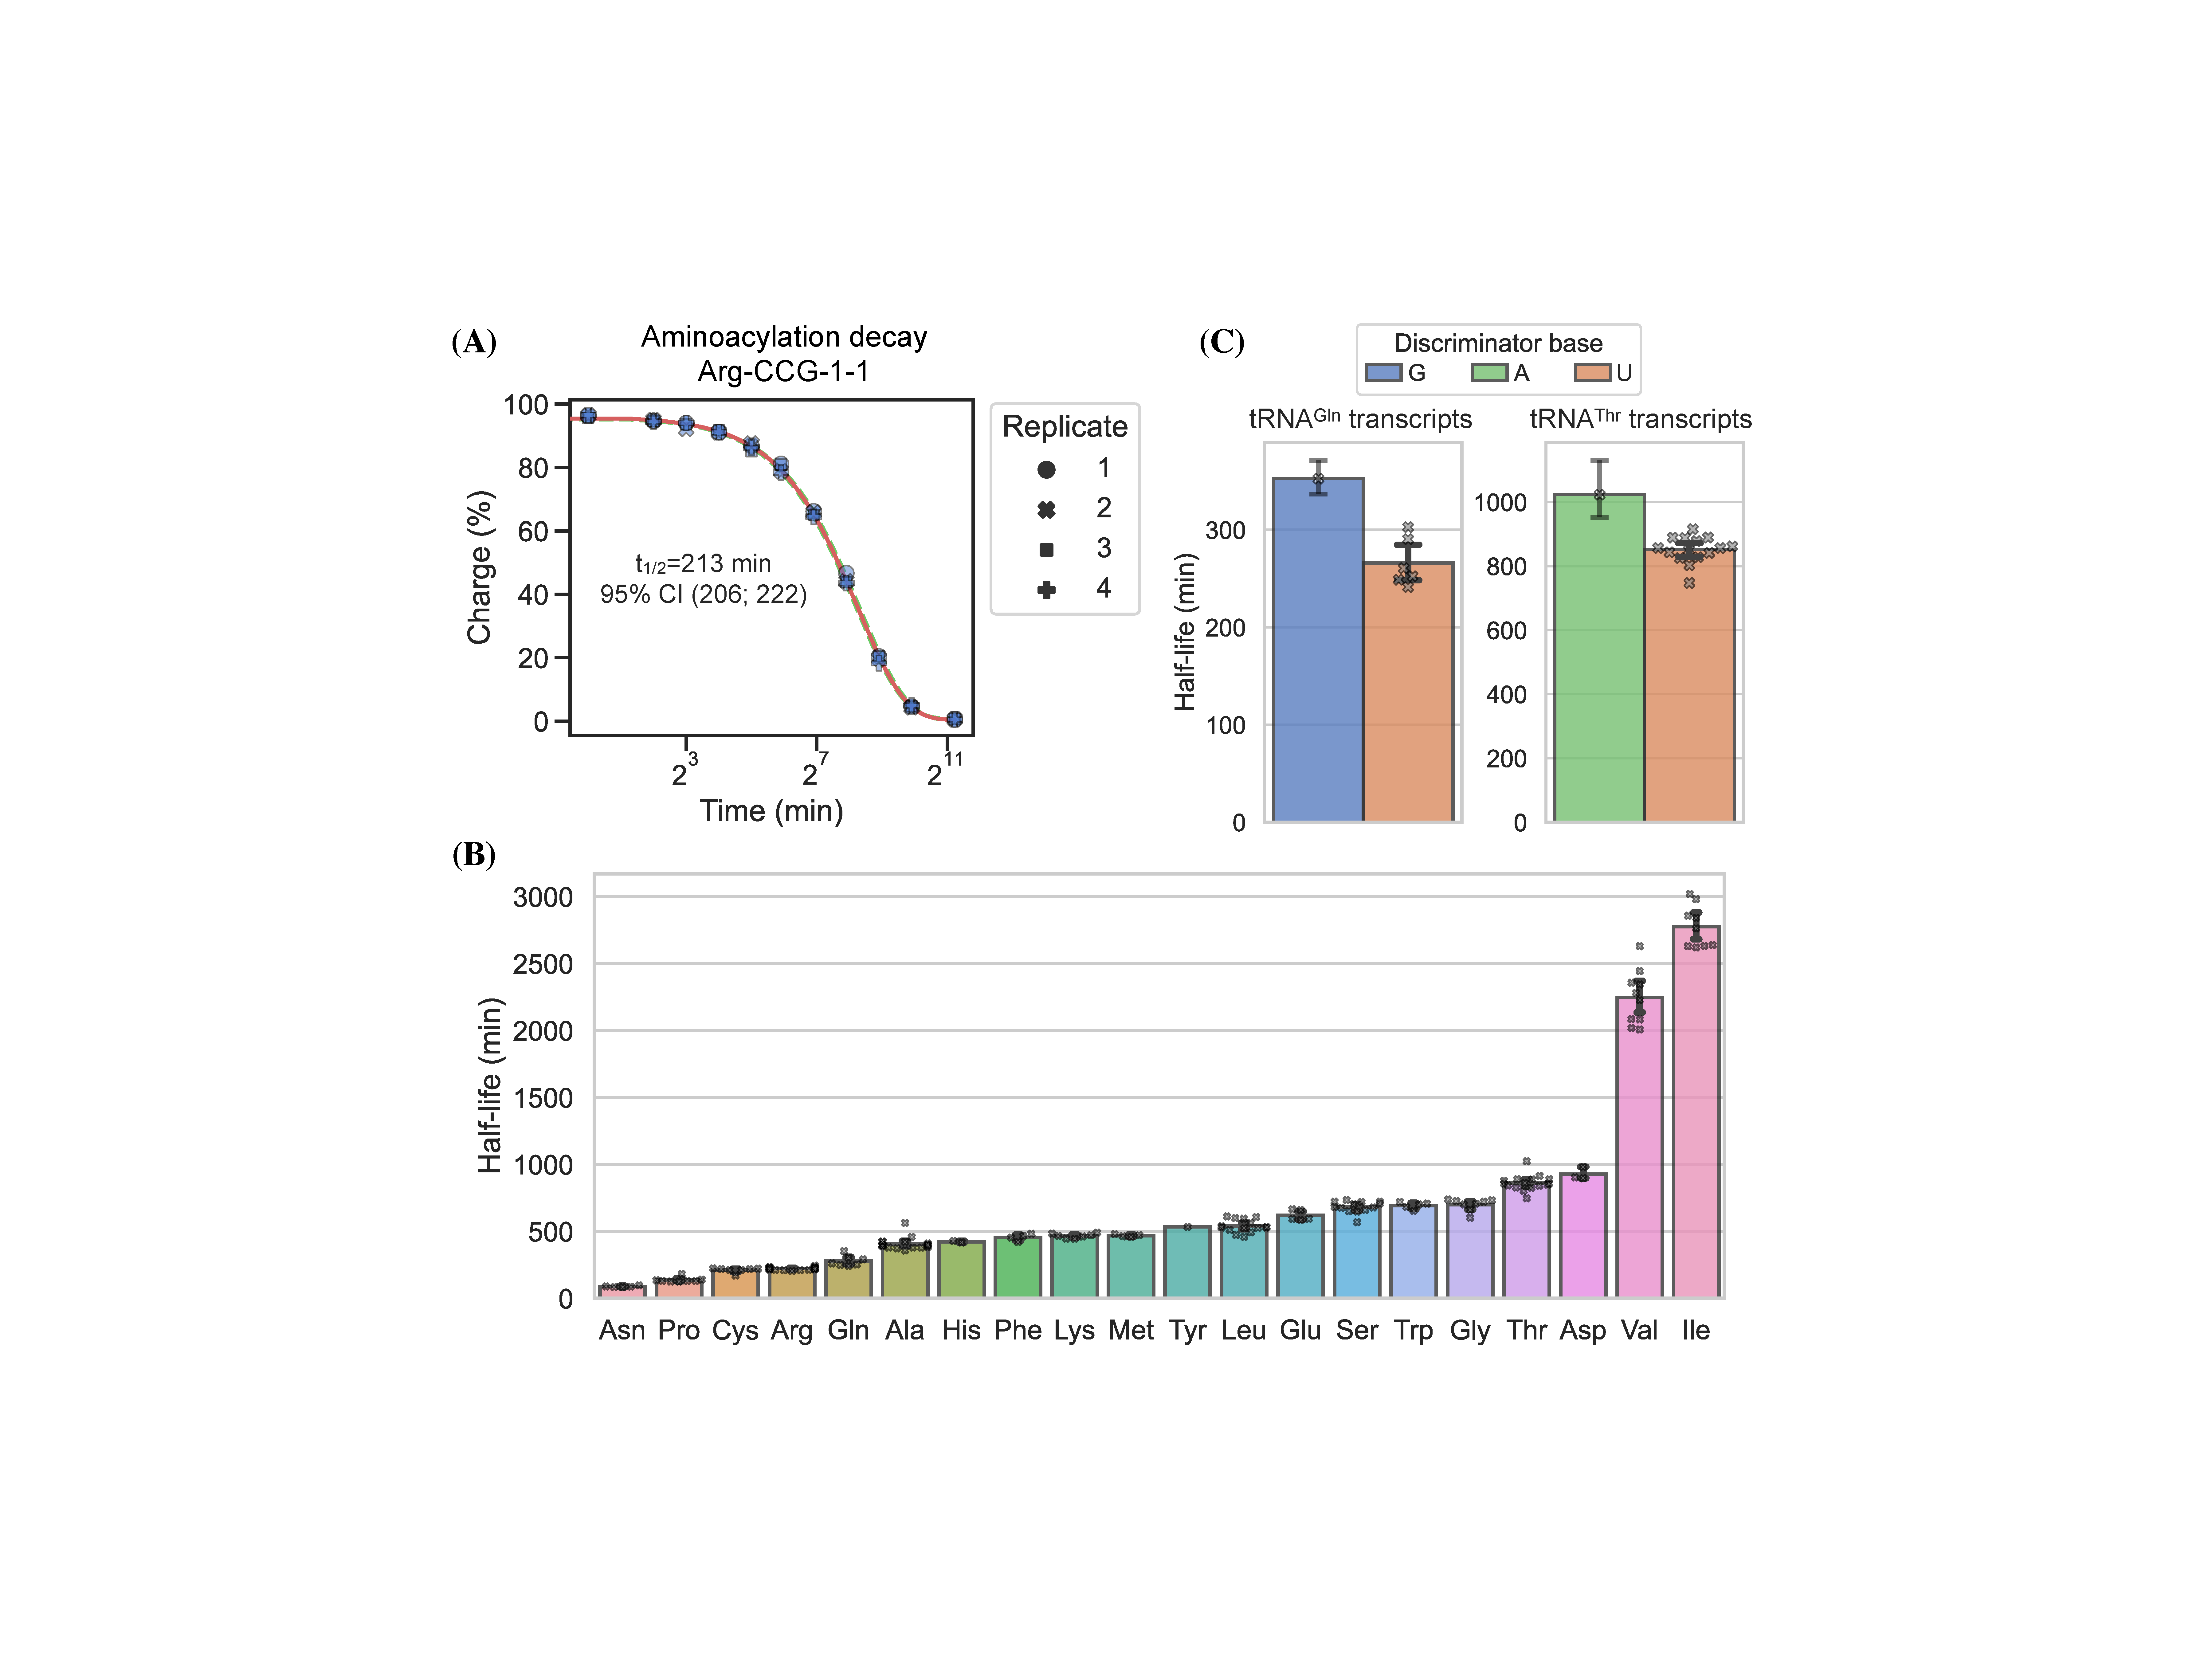
\includegraphics[width=0.70\linewidth]{figures/Fig6.pdf}}
\caption{
Measuring aminoacylation half-life using charge tRNA-Seq.
\textbf{(A)} Aminoacylation decay for a representative tRNA transcript Arg-TCG-2-1 over the 11 timepoints sampled.
For reference, the best and worst fitting tRNA transcripts are shown in \FIGSUPP[Fig6]{f6S2}.
The fitted first-order decay to estimate the aminoacylation half-life is shown as a red line.
Similar dashed lines are plotted in green for the 95\% confidence interval (these are hard to see).
\textbf{(B)} Aminoacylation half-life estimates grouped by amino acid.
Each marker represents one transcript, errorbars are bootstrapped 95\% confidence intervals of the mean.
\textbf{(C)} Distribution of aminoacylation half-life estimates for tRNA\textsuperscript{Gln} and tRNA\textsuperscript{Thr} transcripts grouped by discriminator base identity.
Errorbars are bootstrapped 95\% confidence intervals.
For the single transcripts with G or A discriminator base the bootstrap is performed on measurement replicates while for the U discriminator base it is performed on the transcripts observations.
}
\label{fig:Fig6}

\figsupp[RNA integrity and comparison to previous half-life values.]{
\textbf{(A)} RNA integrity after the last sample was taken (40 h) for the four replicates in the aminoacylation half-life experiment.
\textbf{(B)} Comparison between aminoacylation half-life estimates grouped by amino acid from this study (tRNAseq) and measurements by \cite{Peacock2014-wk} (radiolabeling).
Errorbars are +/- standard deviations.
A linear regression line is shown as a red line.
}{\fbox{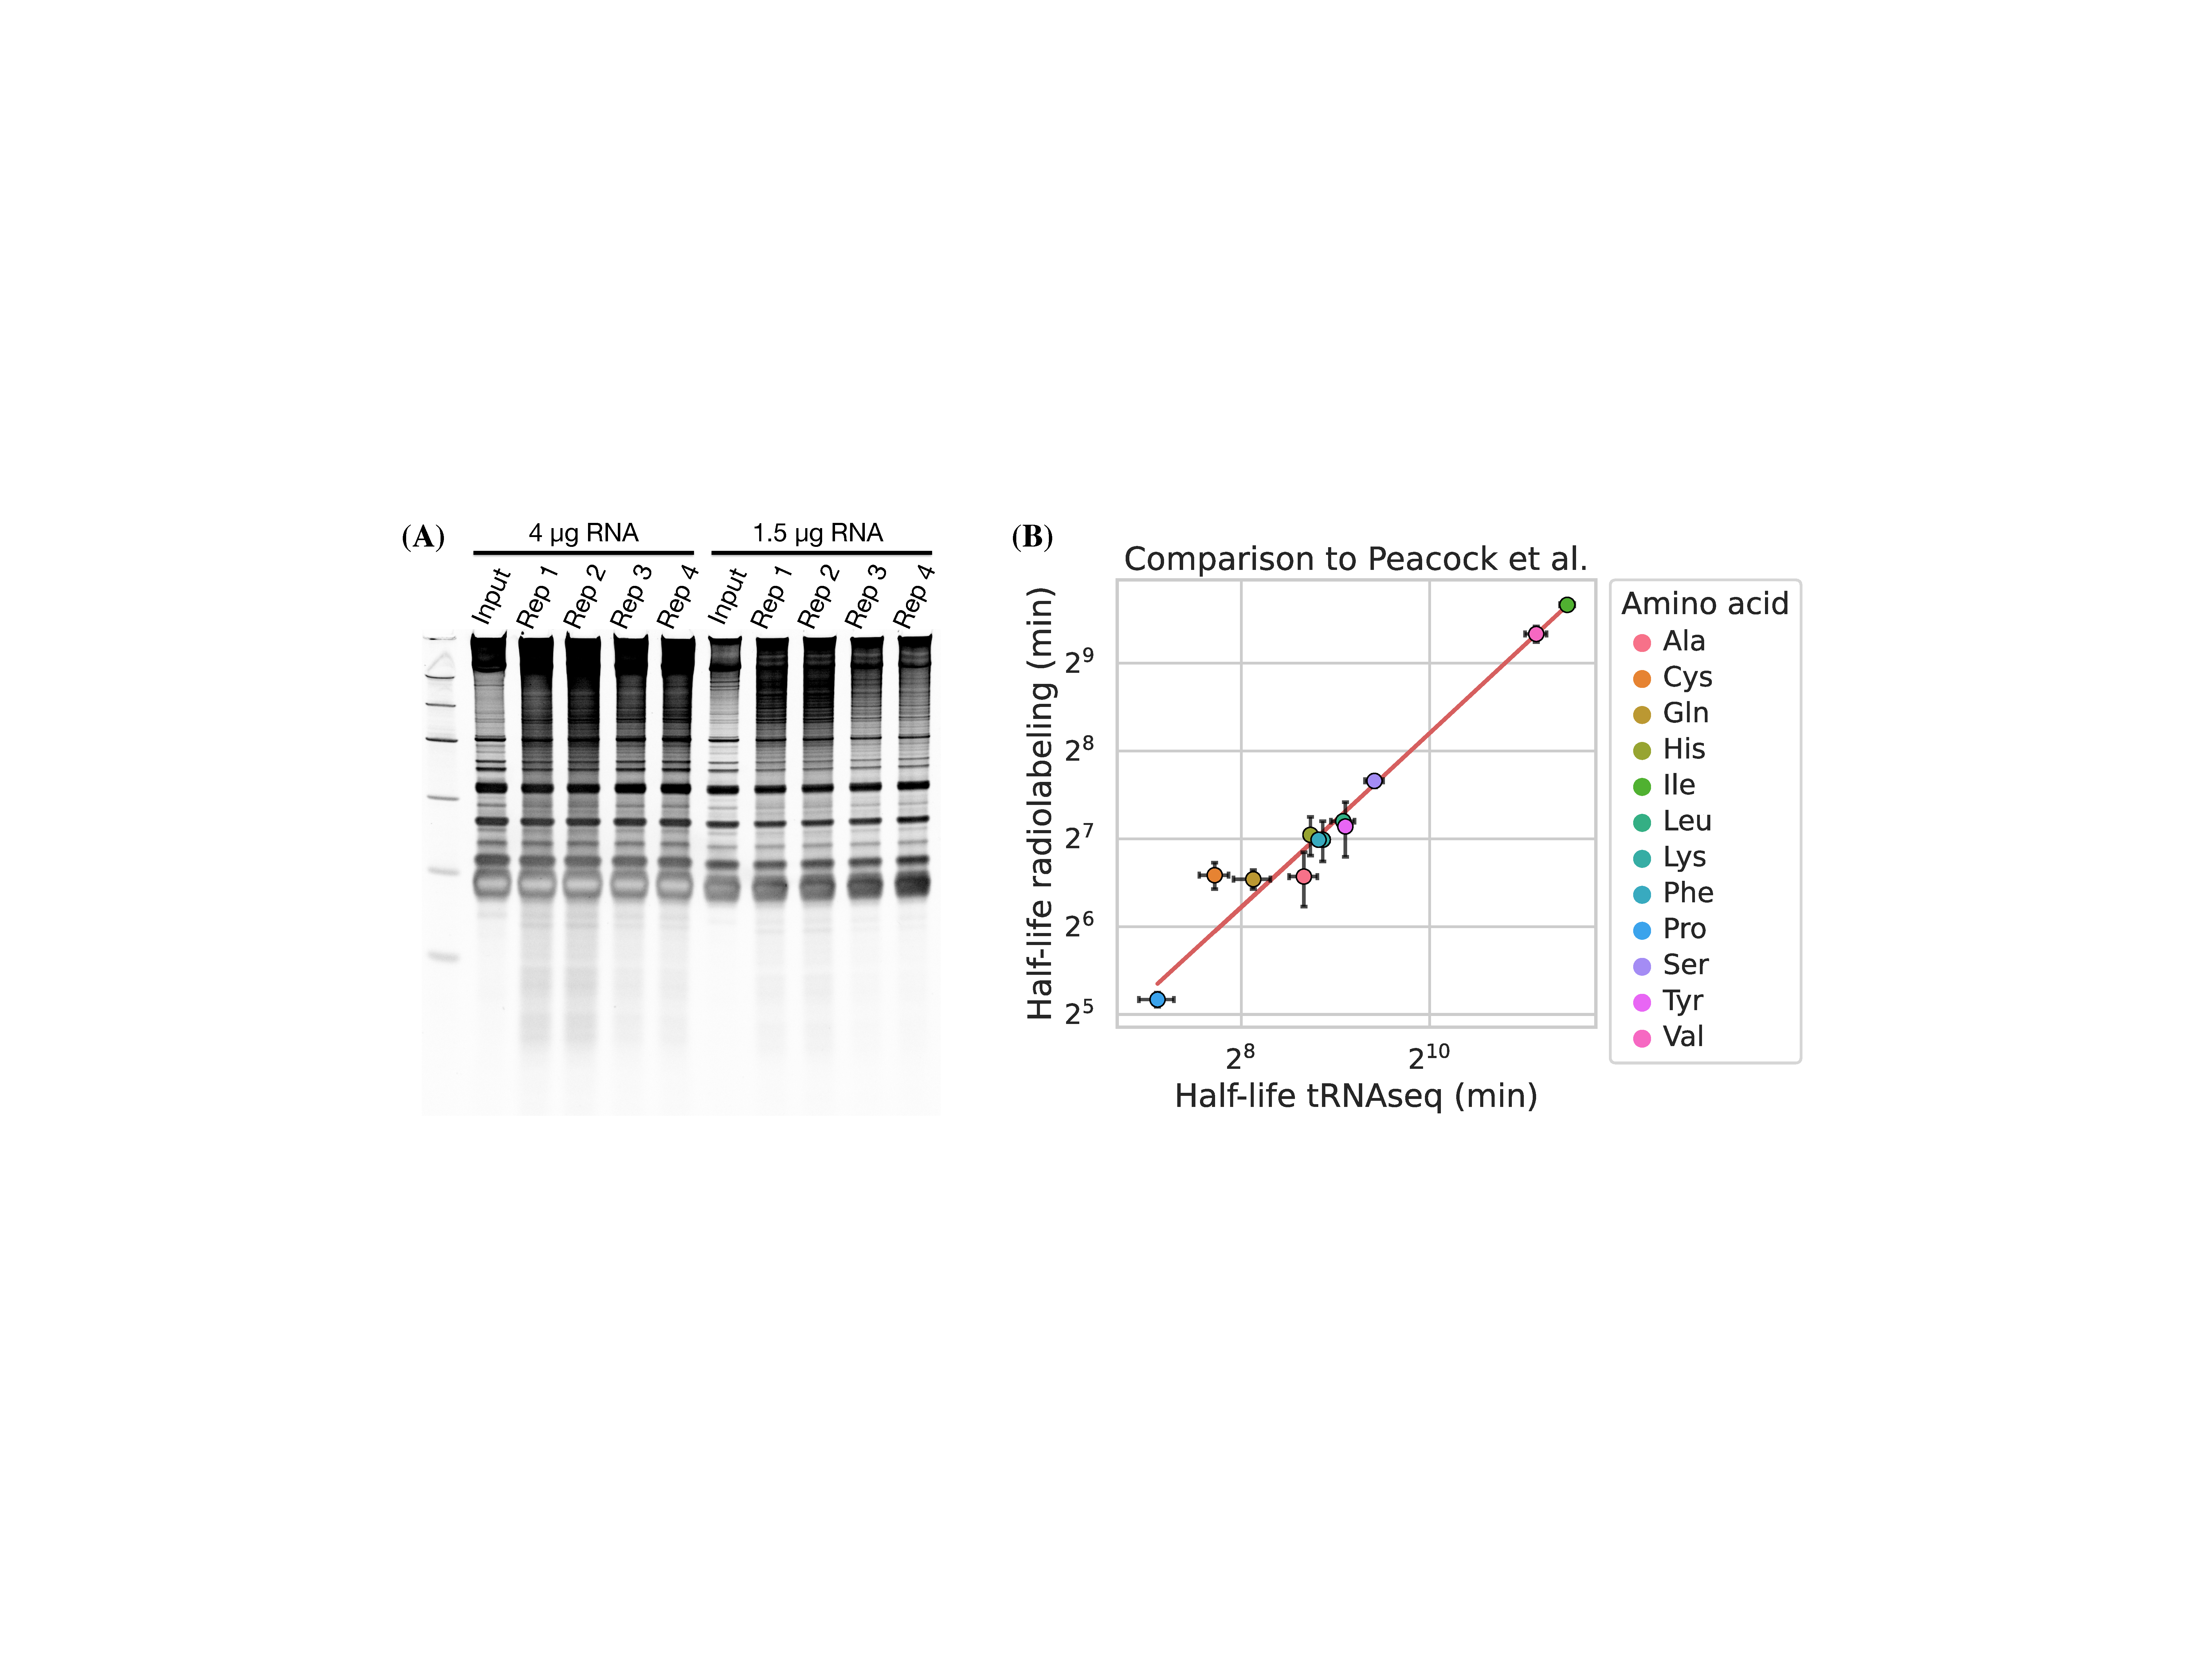
\includegraphics[width=0.85\linewidth]{figures/Fig6S1.pdf}}}\label{figsupp:f6S1}

\figsupp[Best and worst transcript half-life estimates.]{
The best and worst transcript half-life estimates, ranked based on the sum of squared differences between the fitted decay function and the mean charge of the replicates.
Related to the representative (i.e. ranked as the median) transcript shown in \FIG{Fig6}, panel A.
}{\fbox{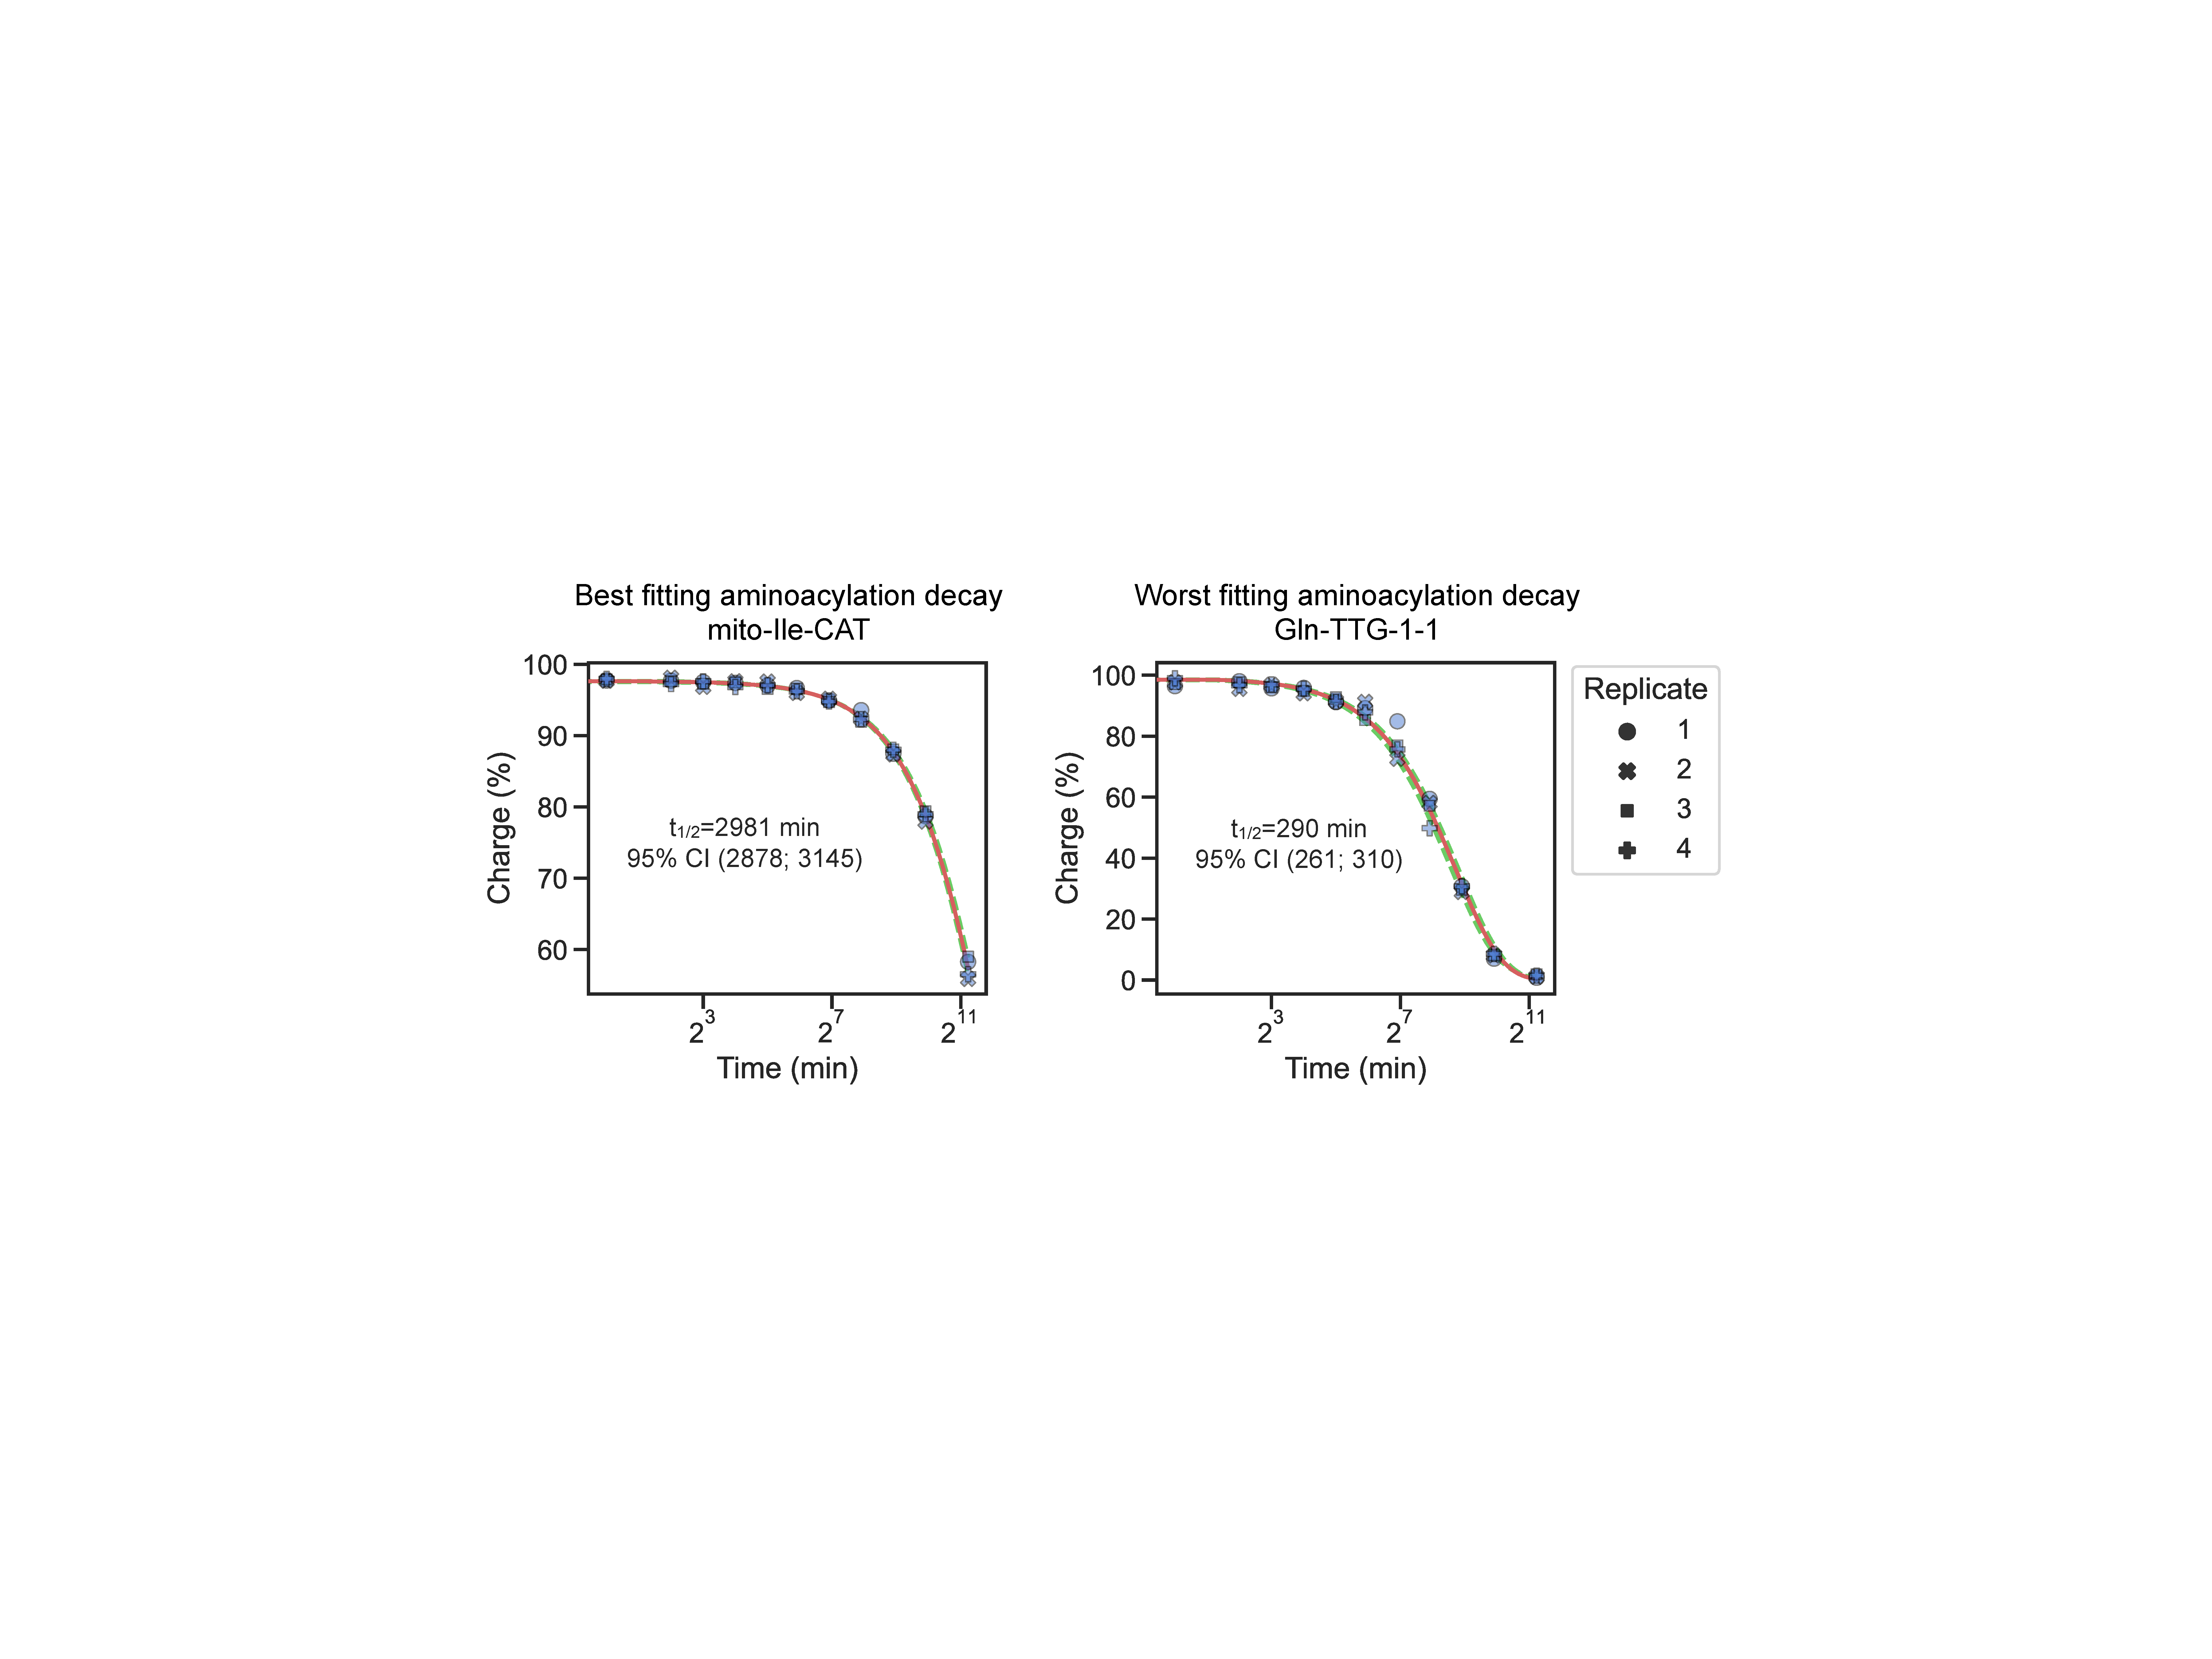
\includegraphics[width=0.85\linewidth]{figures/Fig6S2.pdf}}}\label{figsupp:f6S2}
\end{figure}






\section{Discussion}
Accurate quantification is a prerequisite for making reliable observations standing the test of time and replication.
We have shown a robust method for measuring tRNA charge and done extensive work to validate it in the relevant context of human tRNA.
Furthermore, we have quantified the measurement precision of charge and relative expression.
Accuracy was only quantified for charge measurement whereas this is more challenging for expression levels \citep{Fuchs2015-nb}.
One step towards accurate expression level measurements is efficient adapter ligation, such as the splint assisted ligation method used herein; however, future versions of tRNA-Seq should providing better validation and controls for relative expression measurements.

In our version of the Whitfeld reaction we use lysine to induce base cleavage at low pH.
We later found that ornithine is an even better inducer of cleavage \citep{Uziel1975-ja} and thus, the pH of the cleavage reaction could be lowered even further and possibly combined with Cu\textsuperscript{+2} as a deacylation catalyst \citep{Kroll1952-ci, Schofield1968-qn} to shorten incubation times.

In our experience, as well as others \citep{Shigematsu2017-tv}, splint assisted ligation is highly efficient whereas blunt-end ligation is not.
In contrast, \cite{Behrens2021-gb} achieved high efficiency blunt-end ligation, allowing inclusion of non-mature tRNAs without the normal CCA-end.
The tRNA\textsuperscript{His} is also not suitable for splint assisted ligation due to the additional G added to the 5′ end \citep{Heinemann2012-hq} and thus shielding the discriminator base from base pairing with the splint.
Despite this, reads mapping to tRNA\textsuperscript{His} are surprisingly abundant and both CC and CCA-ending.
In future versions of this method, we see the possibility of combining our optimizations with the on-bead sample processing developed by \cite{Watkins2022-er} to eliminate gel purification steps and achieve faster and cleaner processing.

We solve the tRNA alignment problem by non-heuristic alignment which is guaranteed to return the best alignment.
This is computationally demanding but nevertheless quite possible on the small number of tRNA transcript references.
A more challenging problem is the application of reference masking to improve the annotation accuracy.
We used unique codon annotation as the objective in our optimization of reference masking, but this is a surrogate as the ground truth cannot be determined.
Further improvements could be achieved by simulation of tRNA reads including realistic RT misincorporations, indels and fall off and optimizing alignment to this simulated ground truth.
Additionally, annotation performance could be increased further using tools, such as a as hidden Markov models (HMMs), to model complex phenomena such as interaction between modifications \citep{Wang2021-fc, Hernandez-Alias2022-ch}.

In summary, we report a robust charge tRNA-Seq method that has been thoroughly tested and validated as precise and accurate for charge measurements.






\section{Methods and Materials}
\subsection{Cell culture and RNA extraction}
The human cell line H1299 was acquired from ATCC and tested to be free from mycoplasma (MycoProbe, R\&D Systems).
Cells were maintained in Dulbecco’s Modified Eagle’s Medium (DMEM) supplemented with 3.7 g/L sodium bicarbonate, 10\% fetal bovine serum (FBS) and 1\% penicillin-streptomycin solution.
Cells were incubated in a humidified incubator at 37°C with 5\% CO2.

For RNA extraction, cells were seeded onto a 15 cm dish and grown in DMEM until confluency.
The cells were then removed from the incubator, placed on a slope on ice and media was quickly and thoroughly aspirated before adding 3 mL Trizol to cover all the cells.
From this point onward, everything was kept ice cold to prevent hydrolysis of the aminoacylation.
After a 2 mins incubation, the cell material was scraped down the slope mixing it with the Trizol, then 2x1.5 mL was transferred to 2 mL Eppendorf tubes and 0.3 mL chloroform was added.
The tubes were vortexed 2 min and then centrifuged (17,000g, 5 mins).
From each tube, 0.75 mL of the upper layer was transferred to a tube with 0.8 mL isopropanol (IPA), then mixed and incubated 60 mins at -20°C.
Tubes were then centrifuged (17,000g, 15 mins) and RNA pellets were washed twice with 1 mL 80\% IPA containing 100 mM sodium acetate (pH=4.5).
These washing steps are critical because Trizol contains glycerol which will react with and inhibit the subsequent periodate oxidation step.
A last wash was performed using 1 mL 100\% IPA and after removing the supernatant the RNA pellets were air-dried at room temperature, then stored dry at -80°C.



\subsection{Charge tRNA-Seq using blunt-end ligation}
For charge tRNA-Seq using blunt-end ligation shown in \FIGSUPP[Fig2]{f2S2} the protocol described by \cite{Behrens2021-gb} was followed with the exception of using different adapter sequences, a UMI containing RT oligo (Supplementary file 1), more rounds of amplification and gel based size selection for the final sequence library and using paired-end sequencing.
Briefly, whole cell RNA was extracted, reconstituted in 100 mM sodium acetate (pH=4.5) and concentration adjusted to 1 μg/μL.
A 20 μL sample was move to a new tube and submitted to periodate oxidation and 3′ base elimination using sodium borate as described by \cite{Evans2017-st}.
After purification and reconstitution in water, 8 ng of a 50/50 mix of E.coli tRNA-Lys-CCA and E.coli tRNA-Lys-CC oligo was added as a CCA/CC ratio control.
The true ratio of these oligos is hard to control because each contain a different fraction of truncated oligos that will not contribute to the number of mapped reads; however, the sequenced CCA/CC ratio is an important measure of the sample to sample variance.
Then the RNA was 3′ dephosphorylated using T4 PNK and after another round of RNA purification the tRNA fraction was isolated on a 10\% Urea-TBE gel using SYBRGold staining and a blue light transilluminator for visualization.
After gel elution and reconstitution in water, 100 ng tRNA was transferred to a PCR tube and ligated to 20 pmol pre-adenylated adapter (l1, l2, l3 or l4) in 25\% PEG-8000, 1xT4 RNA ligase buffer using 1 μL T4 RNA ligase 2 (truncated KQ) and 1 μL SuperaseIn.
Adapters were adenylated using the NEB 5′ DNA Adenylation Kit following the manufacturers instruction.
After purification, adapter adenylation was verified using differential gel migration.
Ligation reactions were incubated 6 h at 25°C, pooled by adapter barcode and purified, followed by isolation of the ligation product from unligated tRNA using a 10\% Urea-TBE gel.

After gel elution and reconstitution in water, the RT-PCR reaction was performed as described by \cite{Behrens2021-gb} using a similar RT oligo but with an extra 9 random nucleotides at the 5′-end to act as a unique molecular identifier (UMI).
After the RT-PCR incubation, the remainder of the sample processing follows the charge tRNA-Seq sample processing described below, including cDNA circularization, Illumina P7/P5 sequence attachment and sequencing.



\subsection{Charge tRNA-Seq method optimization}
Optimization of the oxidation, cleavage and dephosphorylation, collectively called the Whitfeld reaction \cite{Whitfeld1953-ca}, was done using oligos E.coli tRNA-Lys-UUU-CCA and E.coli tRNA-Lys-UUU-CC (Supplementary file 1; anticodon omitted from name below).
Both oligos were gel purified on a 10\% Urea-TBE gel to resolve full length from truncated oligos.
First, the time required for oxidation was tested, following the same quenching and borax buffered high pH induced cleavage used described by \cite{Evans2017-st}.
For this, samples of 35 ng E.coli tRNA-Lys-CCA were prepared in 10 μL 100 mM sodium acetate (pH=4.5) and used as substrate for the Whitfeld reaction conversion to E.coli tRNA-Lys-CC.
Reaction progress was monitored on a 10\% Urea-TBE gel by resolving the one nucleotide difference with the substrate, the product and a 50/50 mix as markers.
Also using this approach, we tested using lysine induced cleavage \citep{Khym1961-xf} by swapping the sodium borate used for cleavage with 1 M lysine (pH=8).
The cleavage step also includes deacylation and to verify the completeness of this, four samples of 10 μg whole cell RNA were prepared in 10 μL 100 mM sodium acetate (pH=4.5) and incubated with 50 μL 1 M lysine (pH=8) at 45°C for 5, 30, 90 and 270 min.
Then, 1 mL ice cold 80\% isopropanol containing 100 mM sodium acetate (pH=4.5) was added, RNA was precipitated, washed twice, dried and reconstituted in 10 μL 100 mM sodium acetate (pH=4.5).
These deacylated samples were then submitted to the charge tRNA-Seq sample processing described below, except using lysine at pH=9.5 and 90 min incubation at 45°C to ensure complete deacylation.
Incubation time in lysine (pH=8) was chosen to be 4 h.
To compare the RNA integrity after cleavage with lysine vs. borax, samples of 10 μg whole cell RNA were prepared in 10 μL 100 mM sodium acetate (pH=4.5) and added 50 μL of either 1 M lysine (pH=8) or 100 mM sodium borate (pH=9.5).
Tube were incubated 45°C and samples taken at time 0, 1.5, 4 and 8 h.
RNA integrity was determined using TapeStation (high sensitivity RNA) and 10\% Urea-TBE gel.
Upon combining the steps of the Whitfeld reaction to a one-pot reaction a color change was observed after addition of lysine.
To test the effect of the periodate quencher, 25 μL of freshly prepared 200 mM NaIO4 in 100 mM sodium acetate (pH=4.5) was quenched by 25 μL of either water (control), glycerol \citep{Alefelder1998-ln}, glucose \citep{Evans2017-st}, ribose \citep{Watkins2022-er} or uridine at concentrations indicated for 10 min at room temperature.
Then 50 μL 1 M lysine at either pH 8 or 9.5 was added and reactions incubated at 45°C for 1 h before moving to room temperature for visual inspection (\FIGSUPP[Fig2]{f2S1}, panel C).

For ligation optimization human tRNA was isolated from H1299 cells.
First, whole cell RNA was isolated (described above), reconstituted in water and deacylation at 45°C in 1 M lysine (pH=8) for 4 h.
Then, RNA was purified using the Monarch RNA Cleanup Kit (50 μg) and run on a 10\% Urea-TBE gel to resolve the tRNA from mRNA and rRNA.
tRNA was defined as the range between 70 and 85 nt. as approximated by the low range ssRNA ladder.
For blunt-end ligations in \FIGSUPP[Fig2]{f2S3}, 40 ng tRNA, either isolated from H1299 cells or as tRNA-Lys-CCA oligo, was ligated to 20 pmol pre-adenylated adapter in a 20 μL reaction containing 25\% PEG-8000, 200 U T4 RNA ligase 2 (truncated KQ; Rnl2tr KQ), 10 U SUPERaseIn and the vendor provided buffer.
For splint assisted ligation in \FIGSUPP[Fig2]{f2S4}, 35 ng tRNA, either isolated from H1299 cells or as tRNA-Lys-CC oligo, was ligated to 20 pmol annealed adapter:splint partial duplex as described for charge tRNA-Seq sample processing below.
For the non-complementary splint test, two splint oligos were made with CAAC and AAC overhangs (Supplementary file 1) and annealed to adapter l1Sp.
For the ligation test in \FIG{Fig2}, panel E and \FIGSUPP[Fig2]{f2S5}, panel A, 500 ng tRNA isolated from H1299 cells was subjected to the one-pot Whitfeld reaction described for charge tRNA-Seq sample processing below but with a single step remove.
For the no oxidation sample NaIO4 was replaces with NaCl, for the no dephosphorylation sample shrimp alkaline phosphatase (rSAP) was replaces with water and for the no cleavage sample RNA was purified after periodate quenching.
A parallel sample was processed as described in \cite{Evans2017-st}.
All samples were purified using the Monarch RNA Cleanup Kit and 35 ng was used per ligation test with adapters l1Sp, l2Sp and l3Sp using the ligation protocol as described for charge tRNA-Seq sample processing below.



\subsection{Charge tRNA-Seq sample processing}
Described in details in Supplementary file 2.
Whole cell RNA was reconstituted in 100 mM sodium acetate (pH=4.5) and keep on ice until the end of the periodate oxidation step.
For deacylated control samples, RNA was prepared by first performing a deacylation step on the input RNA by incubation in 1 M lysine (pH=8) at 45°C for 4 h, followed by purification using the Monarch RNA Cleanup Kit (50 μg).
The RNA concentration was adjusted to 1 μg/μL, 10 μL was transferred to a fresh tube and 1 μL E.coli tRNA spike-in control was added.
Initially, the spike-in control contained 5 ng/μL E.coli tRNA-Lys-CCA, later 5 ng/μL of each E.coli tRNA-Thr-CGT CCA-Phos and E.coli tRNA-Thr-CGT CCA was also included.
To this 5 μL freshly prepared 200 mM NaIO4 was added following 10 min incubation on ice, in the dark.
For non-oxidized control samples, NaCl was used instead of NaIO4.
The oxidation was quenched by adding 5 μL 50\% (v/v) ethylene glycol ($\sim$9 M) and incubating for 5 min on ice and 5 min at room temperate, in the dark.
Then 50 μL 1 M lysine (pH=8) with 1 μL SuperaseIn was added and tubes were incubate for 4 h at 45°C.
To dephosphorylate RNA, completing the Whitfeld reaction, 8 μL 10X rCutSmart Buffer and 1 μL rSAP was added followed by 30 min incubation at 37°C.
RNA was then purified using the Monarch RNA Cleanup Kit (50 μg), eluting with 30 μL water.
A 6 μL sample was then denatured by mixing with 2x urea loading buffer (8 M urea, 30 mM sodium acetate, 2 mM EDTA, 0.02 \% (w/v) bromophenol blue and xylene cyanol, pH adjusted to 4.7-5) and incubating 2 min at 90°C.
The tRNA fraction was then isolated on a 10\% Urea-TBE gel using SYBRGold staining and a blue light transilluminator for visualization.
Gel elution was done by crushing the gel with a disposable pestle, adding 200 μL gel elution buffer and 1 μL SuperaseIn, then snap freezing in liquid nitrogen and incubating at 65°C for 5 mins with shaking.
The gel slurry was filtered through a Spin-X filter following tRNA purification using the Oligo Clean \& Concentrator kit.
The concentration of purified tRNA as measured, then it was annealed in  NEBuffer 2 by heating to 94°C for 2 min followed by cooling 1°C/s to 4°C.
35 ng of the annealed tRNA was transferred to a PCR tube and to this was added 20 pmol annealed adapter:splint partial duplex, 1 μL 10x NEBuffer 2, 2 μL 10x T4 RNA ligase buffer, 4 μL 50\% PEG-8000, 1 μL SuperaseIn and 1 μL T4 RNA ligase 2.
The annealed adapter:splint partial duplex was made by making an equimolar mix of the CCA and CC splint oligos, then using this to make an equimolar mix with the adapter oligo and annealing this in NEBuffer 2 by heating to 94°C for 2 min followed by cooling 0.3°C/s to 4°C.
Each ligation reaction was adjusted to 20 μL with water, mixed and incubated 1 h at 37°C followed by 24 h at 4°C and heat inactivation at 80°C for 5 min.
Samples were pooled by adapter barcode, purified using the Oligo Clean \& Concentrator kit and then ligated tRNA was isolated on a gel and purified similarly to the initial tRNA isolation.

Reverse transcription was setup with 60 ng of the purified adapter ligated tRNA as template using the buffer composition, incubation temperature and time suggested by \cite{Behrens2021-gb}.
To 10 μL template in a PCR tube, 2 μL 1.25 μM RT oligo and 4 μL RT buffer was added following denaturation/annealing using 90°C for 2 min, 70°C for 30 s and cooling 0.2°C/s to 4°C.
Then, to each tube 1 μL 100 mM DTT, 1 μL SuperaseIn and 1 μL TGIRT-III RT polymerase (or Maxima H Minus for \FIGSUPP[Fig2]{f2S7}) was added following 10 min incubation at 42°C.
Then 1 μL 25 mM dNTPs was added and the incubation was resumed at 42°C for 16 h on a thermocycler with the heated lid set to 50°C.
The RNA template was hydrolyzed by adding 1 μL 5 M NaOH followed by incubation at 95°C for 3 min.
The samples were then purified using the Oligo Clean \& Concentrator kit and the cDNA was isolated on a gel and purified similarly to the initial tRNA isolation, eluting cDNA using 7 μL water.
cDNA was circularized by transferring 5.5 μL cDNA to a PCR tube and adding 2 μL 5 M betaine, 1 μL 10x CircLigase buffer, 0.5 μL 1 mM ATP, 0.5 μL 50 mM MnCl2 and 0.5 μL CircLigase.
The reaction was incubated at 60°C for 3 h on a thermocycler with a 70°C heated lid, then the enzyme was deactivated by denaturing at 80°C for 10 min.

PCR was used to attach Illumina P7/P5 sequences to flank the tRNA insert.
Each PCR reaction was setup to contain 0.6 μL circularized cDNA, 1.5 μL 10 mM dNTPs, 5 μL 10 μM P7 oligo, 5 μL 10 μM P5 oligo, 10 μL 5x KAPA HiFi buffer, 1 μL KAPA HiFi polymerase and 26.9 μL water.
The PCR reactions were incubated at 95°C for 3 min followed by 3 cycles of 98°C for 20 s, 68°C for 10 s and 72°C for 15 s, and then followed by X cycles of 98°C for 20 s and 72°C for 15 s, with X being empirically determined (\FIGSUPP[Fig2]{f2S8}, panel A).
The optimal number of PCR cycles were determined by preparing three PCR reactions, incubating them with X=10, 12 and 14 and running 4 μL of each reaction on a 4-12\% TBE gel.
The PCR reactions with optimal X, resulting in abundant amplification product with little PCR crossover, were purified using the DNA Clean \& Concentrator-5 kit and resolved on a 4-12\% TBE gel.
The gel was stained using SYBRGold and visualized using a blue light transilluminator to isolated the library DNA by cutting out the size range covering all possible insert lengths (170-290 bp).
Gel elution was done by crushing the gel with a disposable pestle and adding 300 μL TBE, then snap freezing in liquid nitrogen and incubating at room temperature overnight with mixing.
If necessary, elution time could be decreased by incubation at higher temperature; although, this required adding higher salt concentrations to prevent DNA reannealing (\FIGSUPP[Fig2]{f2S8}, panel B).
The gel slurry was filtered through a Spin-X filter following DNA purification using the DNA Clean \& Concentrator-5 kit and eluting with 20 μL 10 mM Tris (pH=8).
DNA with different Illumina P7/P5 barcodes were pooled for multiplexing and sequenced using Illumina paired end sequencing using 2x100 bp reads.



\subsubsection{E.coli tRNA spike-in control}
An E.coli tRNA spike-in control was generated from oligos E.coli tRNA-Lys-UUU-CCA and E.coli tRNA-Thr-CGT-CCAA (anticodon sometimes omitted from name).
First, 2 μg per well of the E.coli tRNA-Lys-CCA oligo was loaded on a 10\% Urea-TBE gel to resolve full length from truncated oligos.
After gel elution and purification using the Oligo Clean \& Concentrator kit the RNA concentration was measured and adjusted such that 5 ng was spiked into each sample of 10 μg whole cell RNA before periodate oxidation.
Adding the control before periodate oxidation afforded an internal control of the completeness of the oxidation reaction.

Second, 30 μL of 100 μM E.coli tRNA-Thr-CCAA oligo was submitted to the partial Whitfeld reaction, stopping before the dephosphorylation step.
The oxidation reaction was performed by adding 10 μL 100 mM sodium acetate (pH=4.5) and 20 μL 200 mM NaIO4 followed by incubation for 30 min at room temperature in the dark.
Oxidation was quenched using 20 μL 50\% ethylene glycol and incubated 30 min at room temperature in the dark.
Then buffer exchange was performed using a P-6 gel column pre-equilibrated with 100 mM lysine (pH=8).
To the eluate 400 μL 1M lysine (pH=8) and 1 μL SuperaseIn was added followed by 5 h incubation at 45°C and purification using the Monarch RNA Cleanup Kit (using two 50 μg columns).
The product, a 1 nt. truncated and 3′ phosphorylated oligo (E.coli tRNA-Thr-CCA-Phos), was resolved on a gel to isolate the full length oligo, as described for the other control.
Half of this product was submitted to dephosphorylation using rSAP and purified using the Oligo Clean \& Concentrator kit yielding E.coli tRNA-Thr-CCA.
Complete phosphorylation of E.coli tRNA-Thr-CCA-Phos and complete dephosphorylation of E.coli tRNA-Thr-CCA was verified using ligation (\FIGSUPP[Fig5]{f5S3}, panel A).
Then concentrations of both E.coli tRNA-Thr-CCA-Phos and E.coli tRNA-Thr-CCA was measured to generate an equimolar mix adjusted such that 10 ng was spiked into each sample of 10 μg whole cell RNA before periodate oxidation.
The 3′ phosphorylation protects from periodate oxidation and thus adding it before periodate oxidation afforded an internal control of a 50\% charged tRNA probing the completeness of the whole Whitfeld reaction and potential adapter ligation bias.



\subsection{Oligo design}
For adapters used for blunt-end ligation the design was similar to \cite{McGlincy2017-ro} and \cite{Behrens2021-gb}, with a 5′ phosphorylation to enable adenylation and a 3′ dideoxycytidine to prevent self-ligation and concatemer formation.
For adapters l1, l2, l3 and l4 the barcode sequence was 8 nt. starting at the 5′, for adapters l1N, l2N and l3N the barcode sequence was truncated to 5 nt. to make space for a preceding six random nucleotides to diversify the sequence context engaged in ligation.

The design of adapters used for splint assisted ligation was influenced by \cite{Smith2015-ht} and \cite{Shigematsu2017-tv} but with several important differences.
The first difference is that we do not use ribonucleotides at any positions in our adapters or splint oligos.
This affords us higher quality adapter oligos due to the higher coupling efficiency of deoxyribose during oligo synthesis as well as robustness against hydrolysis of DNA compared to RNA.
A primary reason to use ribonucleotides in the adapters and splint oligos is to increase ligation efficiency; however, we achieved $\sim$100\% ligation efficiency on isolated human tRNA using our design without ribonucleotides (\FIGSUPP[Fig2]{f2S4}, panel A).
The second difference is that instead of ligating the adapter to the 3′ and the splint to the 5′ of the tRNA, we only ligate the adapter and block the splint from ligation with a 3′ C3 spacer, as well as dephosphorylating the 5′ of the tRNA.
Similar to the blunt-end ligation adapters, a 3′ dideoxycytidine is included on all adapters to block self-ligation and concatemer formation.
The third difference is that we use two different lengths splint oligos with overhang compatible to NCCA and NCC-ending tRNA.
Also, we encode the nucleotide in the splint complementary to the discriminator base (N) as a random nucleotide instead of using four oligos.
The fourth difference is that our adapters vary in length by the size of their barcodes, from 5 to 8 nt.
This will offset the sequencing reading frame of read P2 (P7) as it goes into the 3′ end of the tRNA, thus increasing the sequence diversity and base calling quality.

The RT-PCR oligo was designed similar to \cite{McGlincy2017-ro} and \cite{Behrens2021-gb} with a 5′ phosphorylation for subsequent circular ligation of the cDNA and an 18-atom hexa-ethyleneglycol spacer (iSp18) to terminate the polymerase extension and avoiding rolling-circle amplification during the PCR to attach Illumina P7/P5 sequences.
The RT oligo has a random purine base on the 5′ to increase circular ligation efficiency.
We added an additional 9 random nucleotides following this purine to increase the diversity of the sequence engaged in circular ligation.
The random nucleotides also provide a unique molecular identifier (UMI) with 524288 possible sequences that enable collapsing of reads derived from the same tRNA molecule.
The UMI is also used as a general sample quality control by comparing the number of observed UMI sequences with the number expected.
The number of expected unique UMI observations is calculated as:
\begin{equation}
E[X] = n \left[ 1 - \left(\frac{n-1}{n} \right)^k \right]
\end{equation}
With $E[X]$ being the number expected observations, $n$ being the number of reads for the particular sample and $k$ being the number of possible UMIs.

The final dsDNA library was designed as an Illumina TruSeq dual index library with combined i5 and i7 indices attached by PCR with P7/P5 oligos.
These oligos were synthesized with a phosphorothioate bond between the last two nucleotides to prevent degradation by the KAPA HiFi polymerase.
An overview of the RNA/DNA manipulations including ligation of adapters, RT-PCR, circularization and library PCR is provided in Supplementary file 3.



\subsection{Read processing}
Reads were first demultiplexed according to their i7/i5 barcodes.
Read pairs were then trimmed and merged using AdapterRemoval:
\begin{lstlisting}
AdapterRemoval --preserve5p --collapse --minalignmentlength 10 --adapter1 AGATCGGAAGAGCACACGTCTGAACTCCAGTCAC<P7_index>ATCTCGTATGCCGTCTTCTGCTTG --adapter2 AGATCGGAAGAGCGTCGTGTAGGGAAAGAGTGT<P5_index>GTGTAGATCTCGGTGGTCGCCGTATCATT --minlength <MIN_LEN>
\end{lstlisting}
With \verb|<P7_index>| and \verb|<P5_index>| defined by the i7/i5 index sequences for the given sample and \verb|<MIN_LEN>| set to 25 for charge tRNA-Seq using blunt-end ligation and 39 for splint assisted ligation charge tRNA-Seq.
Each file with merged reads were then split into samples based on adapter barcode.
A read was assigned to a particular adapter barcode if its 3′ end had a substring within a hamming distance of one from the barcode sequence, including the region complementary to the splint.
The adapter sequence was then trimmed off the 3′ end; similarly, the 10 nt. UMI was located, saved and trimmed off the 5′ end, leaving only the tRNA sequence with possible 5′ non-template bases introduced during RT-PCR.
Finally, each sample was randomly downsampled to 2e6 reads if exceeding this number.

Trimmed reads were aligned to a masked reference (described below) using the Smith-Waterman algorithm implemented by SWIPE \citep{Rognes2011-iu}:
\begin{lstlisting}
swipe --symtype 1 --outfmt 7 --num_alignments 3 --num_descriptions 3 --evalue 0.000000001 --strand 1 -G 6 -E 3 --matrix <SCORE_MATRIX>'
\end{lstlisting}
With an input score matrix (\verb|<SCORE_MATRIX>|) defining a match score of 1, a mismatch score of -3 and a score for alignment to a masked reference position (N) of 0.

Alignment results were processed to extract three key data: 1) tRNA charge, 2) relative expression level and 3) mismatches, gaps and RT truncations.
First the alignment was parsed to extract transcript annotation(s), alignment score and other relevant information.
A read was assigned the annotation with the highest alignment score and upon ties up to three annotations were merged.
When reporting data on the transcript level, a unique annotation was required for filtering, when reporting at the codon level multiple annotations were allowed but required to carry the same anticodon and similarly for data on the amino acid level.
Relative expression levels were calculated as reads per million (RPM) with a count correction such that reads with identical sequence and UMI were only counted once.
Charge was calculated using uncorrected counts as this is a relative number.
Mismatches, gaps and RT truncations were extracted by redoing the Smith-Waterman alignment between the read and its unmasked transcript annotation using a match score of 1, a mismatch score of -1, a gap opening score of -2 and a gap extension score of -1.
Using this new alignment, mismatched, gaps and the index at the end of the alignment were extracted.
Then for each transcript the fraction of reads having mismatches and gaps at a given position was calculated and the percentage drop in coverage at each position, referred to here as RT stops, or termination signal by \cite{Wang2021-fc}.
For both mutation, gap fractions and RT stops the UMI corrected read count was used.
For boilerplate example of the whole read processing workflow see \url{https://github.com/krdav/tRNA-charge-seq/blob/main/projects/example/process_data.ipynb}.




\subsection{Reference masking}
A human tRNA transcript reference for alignment was made by downloading the fasta formatted hg38 high confidence mature tRNA sequences from GtRNAdb \citep{Chan2016-wt}.
These sequences were deduplicated and mitochondrial tRNAs and spike-in control sequences were appended.
Then a BLAST database was generated, as required by SWIPE, using the \texttt{makeblastdb} application.
To further improve the alignment specificity, a masked reference was made by converting positions with high likelihood of mismatch to Ns such that these have no negative contribution on the alignment score.
Position-wise mismatch frequency was found as described above and filtered using a minimum of 200 transcript observations and 100 observations on each position.
These were then turned into a masked reference using four tuning parameters for picking the positions to mask.
\verb|unique_anno|: Only count reads with a unique transcript annotation.
\verb|min_mut_freq|: The minimum mismatch frequency to trigger masking.
\verb|frac_max_score|: The minimum fraction of the maximum alignment score between two reference sequences to expand the masked positions in one reference to another, requiring both unmasked positions to have the same nucleotide.
The purpose is for an abundant transcript to donate its masking to a highly similar, but less abundant, transcript likely having the same RNA modifications.
\verb|iteration|: The number of masking iterations to perform.
When changing the reference for alignment by masking the annotations can change, thus changing the position-wise mismatch frequency and the resulting reference masking.
Running multiple iterations of reference masking stabilizes the change.

To find the optimal combination of tuning parameters a grid search was performed, testing all combinations of parameters shown in \FIG{Fig3}, panel A.
The objective for the search is to minimize the percentage of reads assigned to transcripts with multiple anticodons.
Alternatively, the objective could be to minimize the percentage of reads assigned to multiple transcripts; however, this objective can lead the tuning parameters towards masking only a single transcript out of a family of highly similar transcripts, resulting in assignment of unique annotations to truncated reads, which cannot truly distinguish between transcripts of high similarity.
This problem is less concerning using minimization of multiple anticodons since most families of highly similar transcripts have identical anticodons.



\subsection{Barcode replicate test}
For the barcode replicate test shown in \FIG{Fig4}, the RNA used was first incubated 8 h at 20°C in intracellular physiological buffer, similar to the 8 h timepoint described in the aminoacylation half-life section below.
This provided tRNA containing a spectrum of charge levels, spanning from almost fully acylated isoleucine tRNAs to almost fully deacylated asparagine tRNA.
A single 10 μg sample of this RNA was then subjected to the one-pot Whitfeld reaction and subsequent tRNA isolation and ligation to each of the nine adapters as described for charge tRNA-Seq sample processing above.



\subsection{Charge titration test}
Whole cell RNA was reconstituted with 100 mM sodium acetate (pH=4.5) and adjusted to 1 μg/μL while keeping the RNA cold throughout.
Half of this was moved to a fresh tube and deacylated by adding 5x volumes of 1 M lysine (pH=8), incubating at 45°C for 4 h and purifying using the Monarch RNA Cleanup Kit.
Meanwhile the other half was stored at -80°C.
The concentration of the deacylated RNA was adjusted to 1 μg/μL and mixtures of intact and deacylated RNA was made using the following percentages of intact/deacylated RNA: 100/0, 85/15, 70/30, 55/45, 40/60, 25/75, 10/90, 0/100.
Then these mixtures were subjected to the charge tRNA-Seq sample processing protocol described above with between 4 to 8 barcode replicates across independently prepared sequencing libraries, sequenced on different days.

Reads were processed and the aminoacylation charge of each transcript was extracted to relate the measured with the predicted charge.
However, the actual mixing ratios may deviate from the ones noted above due to inaccuracies in measuring the RNA concentration of intact and deacylated RNA, and due to depletion of certain tRNA species during the deacylation process, for example tRNAs sensitive to hydrolysis or depurination.
We address this using a correction factor $F_i$ described below.
To calculate the predicted charge let $A$ represent intact RNA, $B$ represent deacylated RNA and the index $i$ represent the transcript.
Define the concentration, $C$, of a tRNA transcript $i$ in the intact RNA as 1, while letting the concentration of the same tRNA transcript in the deacylated RNA be a fraction, $F_i$, of the intact RNA:
\begin{equation}
\begin{split}
C^A_i = 1 \\
F_i = \frac{C^B_i}{C^A_i} <=> C^B_i = F_i
\end{split}
\end{equation}
Then, define $T^A_i$ as the measured charge of the intact tRNA of a transcript $i$ averaged over the replicates, and similarly $T^B_i$ for deacylated RNA:
\begin{equation}
\begin{split}
T^A_i = \text{Avg charge}(A_i) \\
T^B_i = \text{Avg charge}(B_i)
\end{split}
\end{equation}
Now, the predicted charge of a mixture of $A$ and $B$ can be defined using $p$ to describe the percentage of $A$ in the mixture:
\begin{equation}
\label{eq:pred_charge}
T^{AB}_i(p) = \frac{p T^A_i + (100-p) T^B_i F_i}{p + (100-p) F_i}
\end{equation}
In the above, only $F_i$ is unknown.
The titration was made with 8 different mixing ratios, two of which are used to calculating $T^A_i$ and $T^B_i$, thus leaving 6 mixing ratios, each with several barcode replicates, to fit $F_i$.
Fitting was performed by minimizing the sum of squared differences between predicted and measured charge using the Broyden–Fletcher–Goldfarb–Shanno (BFGS) algorithm with upper and lower bound constraints of 4 and 0.25.
Then using \EQ{pred_charge} the differences between predicted and measured charge was found and broken down by adapter barcode to investigate ligation bias.



\subsection{Aminoacylation half-life}
Whole cell RNA was reconstituted with 1 mM sodium acetate (pH=4.5) and adjusted to 1.5 μg/μL while keeping the RNA cold throughout.
A zero timepoint was then taken and 80 μL was transferred to a PCR tube after which the experiment was started by adding 20 μL room temperature 5x buffer, quickly mixing and placing the tube on a thermocycler set to 20°C.
The buffer used was an intracellular physiological buffer at 1x containing: 19 mM NaCl, 125 mM KCl, 0.33 mM CaCl2, 1.4 mM MgCl2, 0.5 mM spermidine, 30 mM HEPES, adjusted to pH=7.2 with KOH.
Time from start of incubation was tracked and samples drawn at the following timepoints: 4 min, 8 min, 16 min, 32 min, 1 h, 2 h, 4 h, 8 h, 16 h, 40 h.
For the 40 h timepoint, two samples were drawn: one standard and one receiving shame (NaCl) oxidation.
Sample were taken by removing 8 μL, mixing it in a prepared tube with 2 μL ice cold 500 mM sodium acetate (pH=4.5) and storing it at -80°C until all timepoints were collected.
This was repeated four times to generate independent replicates.
Then samples were processed similar to the charge tRNA-Seq protocol described above, but with the three 5 min incubation times during oxidation and quenching increased to 30 min each due to the lower periodate solubility in the presence of potassium ions.

After read processing and alignment, data integrity was verified by checking that the E.coli tRNA spike-in control and the non-oxidized 40 h samples conformed to expectation.
RNA integrity at the end of the experiment was also verified on a gel (\FIGSUPP[Fig6]{f6S1}, panel A).
The aminoacylation charge was then calculated at the codon level and the data fitted to an equation describing first-order decay:
\begin{equation}
N(t) = N_0 \left( \frac{1}{2} \right) ^\frac{t}{t_{1/2}} + N_{\infty}
\end{equation}
Where $N(t)$ is the charge of a given codon as a function of time, $N_0$ is the charge at time zero and $t_{1/2}$ is the decay half-life.
We added the $N_{\infty}$ parameter to model the lower asymptote of the charge to accommodate the small fraction of tRNAs that still presents with a CCA-end after full deacylation.
The three parameters were fitted to the data by minimizing the sum of squared errors using the Broyden–Fletcher–Goldfarb–Shanno (BFGS) algorithm with upper and lower bound constraints for $N_0$ between 100 and 0 percent, for $t_{1/2}$ between 1e5 and 1 min and for $N_{\infty}$ between 3.5 and 0 percent.
A point estimate for the three parameters were found using all timepoints and replicates and a 95\% confidence interval was found using bootstrapping (N=1000) by sampling a single time-series made up of random draws from the replicates (Supplementary file 4).



\subsection{Data availability}
Plots with Seaborn.
Boxplots are plotting with quartile boxes and whiskers covering the remainder of datapoints within a maximum of 1.5 times the inter-quartile range.

Raw data and code for processing uploaded to:
[some data dump link]

Python code available on Github:
\url{github.com/krdav/tRNA-charge-seq}



\section{Acknowledgments}
We would like to acknowledge Arvind Rasi Subramaniam for suggesting we setup charge tRNA-seq, Alicia Darnell for sharing relevant samples and data and David Sokolov for help with early method optimization.



\section{Funding}
L.B.S. acknowledges support from the National Institute of General Medical Sciences (NIGMS; R35GM147118).


\bibliography{main}
\end{document}
